\documentclass[11pt]{report}
\usepackage{unhthesis}
\usepackage{amssymb}
\usepackage{amsmath}
\usepackage{graphicx}
\usepackage{subfigure}
\usepackage{enumerate}
\usepackage[round]{natbib}
\usepackage{mathtools}
\usepackage{setspace}
\usepackage[table]{xcolor}

\usepackage{verbatimbox}

\usepackage[toc,page]{appendix}

\renewcommand{\citep}[1]{\citeauthor{#1}~(\citeyear{#1})}
\renewcommand{\cite}[1]{(\citeauthor{#1},~\citeyear{#1})}

\newcommand{\answerText}[2][red]{\textcolor{#1}{\textit{#2}}}

\makeatletter
\newcommand{\redub}{}
\def\redub#1{%
  \@ifnextchar_%
    {\@redub{#1}}
    {\@latex@warning{Missing argument for \string\redub}\@redub{#1}_{}}%
}
\def\@redub#1_#2{%
    \colorlet{currentcolor}{.}%
    \color{red}%
    \underbrace{\color{currentcolor}#1}_{\color{red}#2}%
    \color{currentcolor}%
}
\makeatother


\hyphenation{Hu-go}
%\hyphenation{Mi-s\'e-ra-bles}

\begin{document}


\title{Using Interactive Visualization to Enhance Understanding of a Fisheries Model}     % Your title
\author{Carmen Rose St.\ Jean}				   % Your name
\prevdegrees{B.S., University of New Hampshire, 2010}
\major{Computer Science}				   % Your new major
\degree{Master of Science}				   % Your new degree
\degreemonth{September}					   % When awarded.
\degreeyear{2014}					   %
\thesisdate{\today}					   % Date of document.
\DOCUMENTtype{THESIS}                          % or DISSERTATION
\Documenttype{Thesis}                          % or Dissertation
\documenttype{thesis}                          % or dissertation
\maketitle     
                                                        % APPROVAL PAGE
                                                        %======================
\supervisor{Colin Ware}{Professor of Computer Science}    % <- One of these
\committee{R. Daniel Bergeron}{Professor of Computer Science}     % <- As many as
\committee{Matthew Plumlee}{Affiliate Assistant Professor in Computer Science}    %    you need...
\makeapproval 

\begin{dedication}
\begin{center}
To my parents.
\end{center}
\end{dedication} 

\begin{acknowledgments}
I would like to thank God for this opportunity to do this thesis and for the ability to complete it.

It was a great privilege to work under my advisor Colin Ware, whom I must thank for his encouragement, mentoring, and patience throughout the entire journey of writing my thesis.  His insights, criticisms, and faith in me over the last year helped me become a better researcher and a more confident person.

I also want to thank my committee member, Matt Plumlee, who was especially helpful during the beginning of this research.  I must also thank my committee member Dan Bergeron for supporting this thesis.  Both of them were helpful with their advice and kindness over the course of this thesis and also during my entire time at UNH.

Thank you also to Michael Fogarty and Robert Gamble for creating the MS-PROD model and for the great collaboration over the past year.  I appreciate all of the ideas and feedback and I hope that this visualization will be helpful to you.

I am deeply grateful to John Kelley and Jason Greenlaw for their support and guidance both during and beyond my nowCOAST time.  They introduced me to Colin Ware and helped me realize what I was capable of by providing me with challenging opportunities.

I owe my thanks to Phil Hatcher, for knowing I was capable of completing a master's degree before I did.  I would also like to express my appreciation to Mark Bochert for my year as his teaching assistant.  Thank you also to Mezgeb for providing feedback and good company during this thesis endeavor.

I am indebted to my father, my mother, Uncle Roger, Danielle, Amanda, and Eric for getting me to where I am today.  Last but not least, thank you especially to Chris, for encouraging me to go back to school and providing me with reassurance whenever I felt overwhelmed.  

\end{acknowledgments}


\tableofcontents					% Always needed...}
%\listoftables						% Delete if no tables.
%\addcontentsline{toc}{section}{LIST OF TABLES}
\listoffigures						% Delete if no figures.
\addcontentsline{toc}{section}{LIST OF FIGURES}

% Abstract page
\begin{abstractpage} 

Fishery management is the science of setting rules for governing fishing so that it is done in a sustainable manner.  An ecosystem-based fisheries management (EBFM) approach has been advocated to recognize ecosystems as the complex systems that they are.  If EBFM is to be put into effect, then fishery managers require ecological models which take many factors into account. MS-PROD is one such model; it is a multi-species production model which forecasts the biomass of ten species of fish in the Gulf of Maine over 30 years.  In the model, the biomass of each fish species depends on effects from harvesting and interactions with the other fish species.  An interactive visualization to the model was designed and implemented to allows the user to investigate the impact of changes in fishing effort in real time.  By combining time series with a network representation, this visualization shows the predicted biomasses of the fish, the changes in biomass that can result from changes in fishing effort, the causal relationships that help to explain the effects of changes in fishing effort, and the uncertainty of the model.  An evaluation was conducted to compare four different methods for depicting the causal relationships in the model---predation and competition---which found that representing those relationships with arc diagrams enhanced understanding of the model.  This visualization is a novel combination of features which may be a powerful tool that could help fishery managers make informed decisions.

\end{abstractpage}

% See UNHTHESIS.TEMPLATE for additional comments about this file.
%

\chapter{Introduction}                % <- Your first chapter title.

\pagenumbering{arabic}
\renewcommand{\thepart}{{\Roman{part}}}				% <- Do this command only for
                                                %    the first chapter!

Fishery managers have only one ``lever'' to pull when it comes to fishery management: the ability to set harvest quotas.  Fishermen work within these quotas by exerting various levels of fishing effort.  Both managers and fisherman can better understand the ecosystem they work within and the implications of their decisions with the assistance of a production model.  In this context, a production model is a mathematical model, based on data, that simulates interactions between species and predicts species biomass as a function of fishing effort, climate change, and other variables.  MS-PROD is a multispecies production model developed by NOAA scientists Gamble and Link \cite{gamble2009}.  A visualization may enhance such a model by making its inner workings more explicit and may be useful for decision making. The goal of this research has been to explore design alternatives and evaluate the effectiveness of different modes of portrayal and interaction to make a visualization of the MS-PROD model that will be a valuable tool to the modelers and stakeholders alike. 

\section{Models}

Both the short- and long-term effects of human exploitation on an ocean ecosystem, such as the species inhabiting the Gulf of Maine, are not easily understood since experiments which would allow ecosystem managers to investigate the impact of different levels of exploitation over many years are either impractical or impossible to conduct on a large scale.  Fortunately, ecosystem models can be used instead to help gain a better understanding of an ecosystem.

\subsection{Lotka-Volterra Equations}

Ecosystem models are abstract representations of an ecological system, and can range from an individual species in its environment to an entire community of species.  A classic example is the Lotka-Volterra model, which is a pair of differential equations for describing the non-linear interactions between a predator species and a prey species. \cite{lotka1926, volterra1926}:

\begin{align}
   \frac{d N_1}{dt} &=   N_1 \left(\alpha - \beta  N_2\right) 
\\ \frac{d N_2}{dt} &= - N_2 \left(\gamma - \delta N_1\right)
\end{align}
where $N_1$ is the number of prey, $N_2$ is the number of predator, $t$ is time, $\alpha$ is the prey's growth rate, $\beta$ is the rate at which the predator destroys the prey, $\gamma$ is the death rate of the predator, and $\delta$ is the rate at which the predator increases from consuming the prey.  The model can be generalized to discuss an arbitrary number of species rather than just a single pair.

The Lotka-Volterra model can be modified to take competition instead of predation into account, as in the Rosenzweig-MacArthur model \cite{rosenzweig1963} and the Leslie-Gower model \cite{leslie1960}.  These adaptations to the model also consider carrying capacity, which is the maximum number of a species that can be sustained indefinitely in a particular environment:

\begin{align}
   \frac{d N_1}{dt} &= r_1 N_1 \left(1 - \left(\frac{N_1 + \alpha_{12} N_2}{K_1}\right)\right)
\\ \frac{d N_2}{dt} &= r_2 N_2 \left(1 - \left(\frac{N_2 + \alpha_{21} N_1}{K_2}\right)\right)
\end{align}
where $r_i$ is the growth rate for species $i$, $K_i$ is the carrying capacity for species $i$, and $\alpha_{ij}$ is the effect species $j$ has on species $i$.  As with Lotka-Volterra, this model concerns only two species, but it can be generalized to include more than two.

Both Lotka-Volterra and Leslie-Gower do not incorporate a factor which is critical when discussing fisheries management: the effect of harvest.  The Schaefer model adds a term to account for the effect of harvest on an individual species \cite{schaefer1957}:

\begin{align}
   \frac{d N}{dt} &= r N \left(1 - \left(\frac{N}{K}\right)\right) - q E N
\end{align}
where $N$ is the number (or biomass) of the species, $r$ is the growth rate, $K$ is the carrying capacity, $q$ is the catchability coefficient, and $E$ is the fishing effort.

Simple models, when available and correct, are generally preferred; since fewer components are needed to describe their real-world counterparts, they are more easily understood and implemented.  All three of these models are subjectively simple in that they only consider a few ecological factors each. However, in reality, ecosystems are complex systems which require management that recognizes them as such \cite{christensen1996}.  Thus, a more holistic approach called ecosystem-based fishery management (EBFM) has been advocated \cite{united1999}.  However, this approach has not often been implemented due to a lack of models which consider all necessary ecological factors.  Gamble and Link developed a multispecies production model (MS-PROD) to fill this gap \cite{gamble2009}.

\subsection{The MS-PROD Model}

The MS-PROD model forecasts biomass for species separated into functional groups, which are biological groupings of species that perform similar functions within their ecosystem.  The model is built upon the Schaefer production model and also includes Lotka-Volterra terms for predation, Leslie-Gower terms for competition, and carrying capacities for functional groups ($K_G$) as well as for the entire system ($K_{\sigma}$):

\begin{align}
\frac{d N_i}{dt} &= r_i N_i \left(1 - \frac{N_i}{K_G} - \frac{\displaystyle\sum\limits_{j=1}^g \beta_{ij} N_j}{K_G} - \frac{\displaystyle\sum\limits_{j=1}^G \beta_{ij} N_j}{K_{\sigma} - K_G}\right) - N_i \displaystyle\sum\limits_{j=1}^P \alpha_{ij} N_j - H_i N_i
\end{align}
where $N_i$ is the number (or biomass) of species $i$, $t$ is a unit of time, $r_i$ is growth rate for species $i$, $\beta_{ij}$ is the competition of species $j$ on $i$, $\alpha_{ij}$ is the predation of species $j$ on $i$, $H_i$ is the harvest rate on species $i$, $g$ is the number of species within species $i$'s group, $G$ is the number of groups, and $P$ is the number of predators.

This model is distinguished from other multispecies production models by describing stocks with explicit ecological and harvest factors.  Each species to be included in the simulation must be specified in the parameter file by listing growth rate, functional group membership, initial biomass, carrying capacity, and catchability.  Additionally, matrices representing inter-species relationships must be provided to describe the relationship between every pair of species.  Such matrices are required for \textit{predation}, where one species consumes the other, and \textit{competition}, where one species affects the other in any manner besides predation.  (In ecology, the word ``interaction'' is often used instead of ``competition,'' but we have chosen to use ``competition'' so that the term ``interaction'' will not be overloaded since ``interactive'' has a separate meaning in a visualization context.)

The MS-PROD authors provided us with a parameter file which listed ten key species chosen from the Northeast United States Continental Shelf Large Marine Ecosystem (NEUS LME), listed here by functional group:%, predation with each of the other species, and interaction with each of the other species.  
\begin{itemize}
	\item \textbf{Elasmobranchs:} Skates, Spiny Dogfish
	\item \textbf{Flatfish:} Windowpane, Winter Flounder, Yellowfin Tuna
	\item \textbf{Groundfish:} Cod, Haddock, Redfish
	\item \textbf{Small Pelagics:} 	Herring, Mackerel
\end{itemize}
%Given an input parameter set of initial biomass values, a predation matrix, an interaction matrix, catchability values, and harvest effort values,
The MS-PROD model runs simulations for 30 years with an annual time step to predict individual biomasses.  While this outputted information is potentially valuable to fishery managers, it was lacking an interactive graphical user interface.  

\section{Visualization Methods}

When designing a visualization, there can be several techniques for visualizing a feature that are worth comparing.  This section reviews existing research of visualization methods which have particular relevance to the problem of creating an effective interface to a fisheries ecosystem model.

\subsection{Time Series}

Fisheries management is focused on the sustainability of choices concerning fish stocks.  A main purpose of ecosystem management is to ensure that future generations can enjoy the same natural resources \cite{christensen1996}.  As such, the MS-PROD model provides biomass forecasts for 30 years.  Therefore, time-oriented visualization techniques must be explored.

Frank categorized time-oriented data as follows \cite{frank1998}: 
\begin{enumerate}
	\item Linear vs. cyclic
	\item Time points vs. time intervals
	\item Ordered time vs. branching time vs. time with multiple perspectives
\end{enumerate}
Aigner et al. point out that techniques for visualizing branching time and time with multiple perspectives are unfortunately uncommon \cite{aigner2008}, but a line chart---a technique frequently used for ordered time data---serves as a good starting point.

%The MS-PROD data consist of discrete time points with definite starting and ending points, falling under the linear time and time points categories.  As for the third criterion, the model outputs one ordered time result for a single execution, however fisheries managers may like to compare alternative scenarios.  Therefore, our domain falls into the branching time category, though in a limited sense. 

\subsubsection{Line Charts}

\begin{figure}[h]
	\centering
	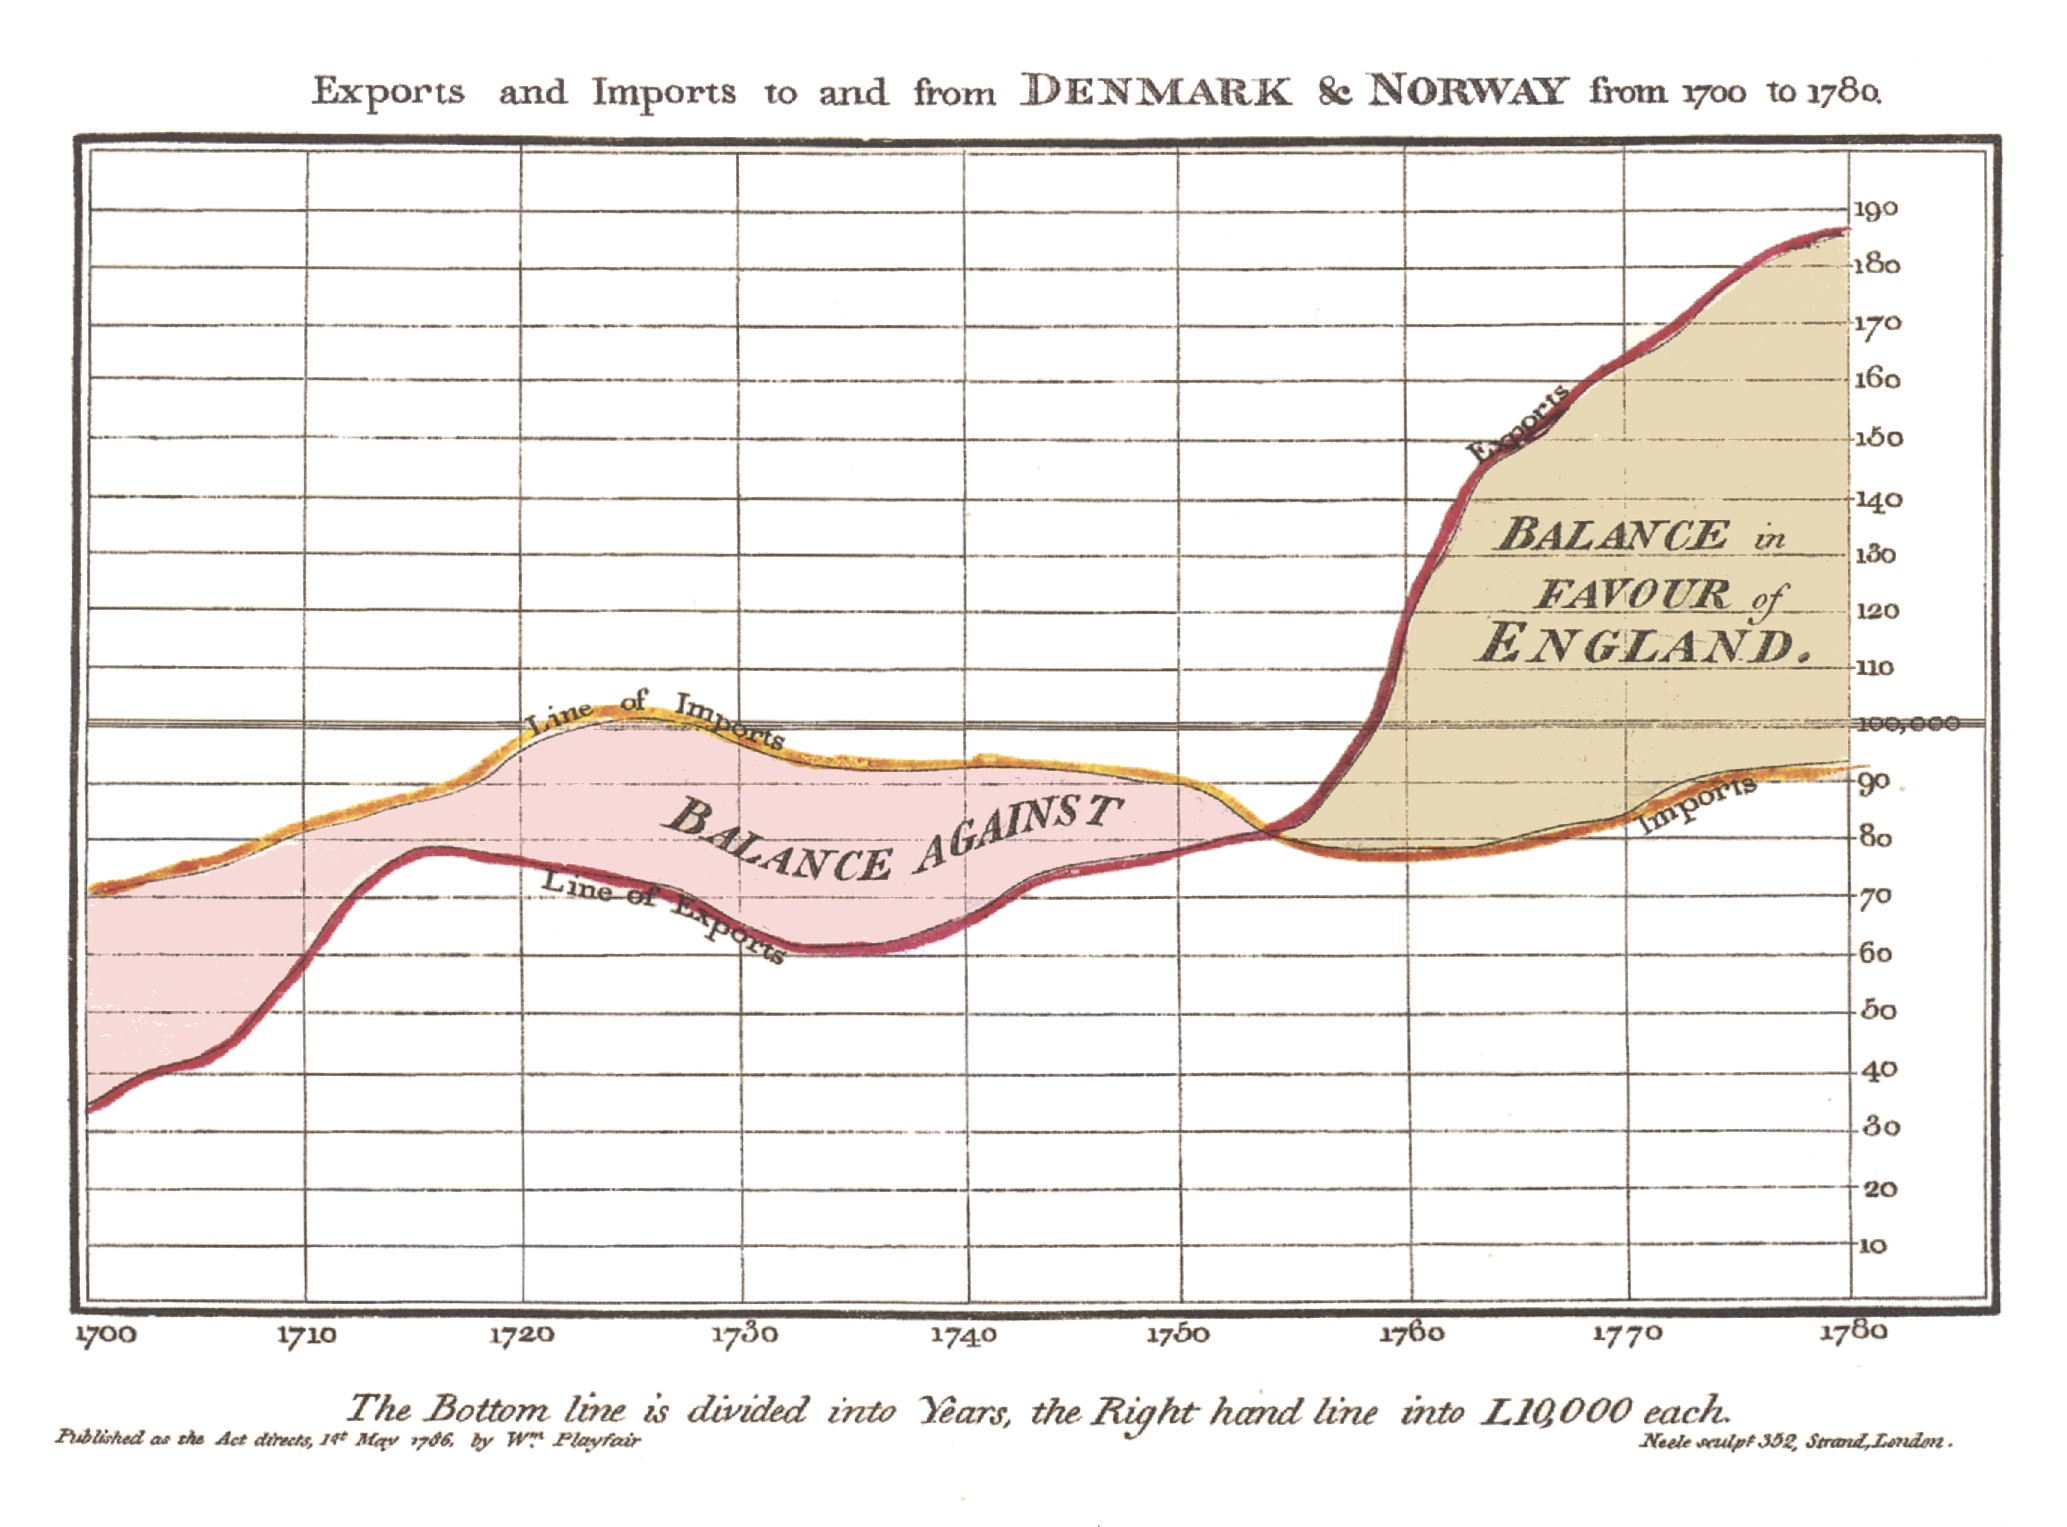
\includegraphics[width=0.9\textwidth]{figures/eps/PlayfairTimeSeries.eps}
	\caption{Playfair's original time series chart \cite{playfair}.}
	\label{fig:playfair}
\end{figure}

The line chart was first invented by William Playfair in 1786 to communicate time series data, seen in Figure~\ref{fig:playfair} \cite{playfair}.  Today, it remains a common method for visualizing time-oriented data in many fields, including science, economics, planning, and engineering to name a few.  Line charts typically encode time on the horizontal axis, progressing from left to right, and some time-varying value on the vertical axis.  Points in the chart are connected by line segments such that the slope of the line indicates the rate of change between time steps.  

\begin{figure}
	\centering
	\begin{subfigure}[b]{0.45\textwidth}
		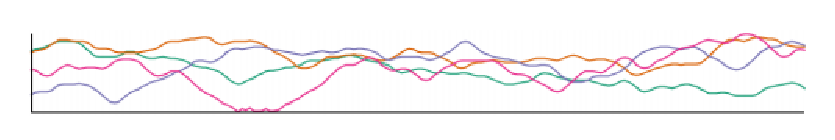
\includegraphics[width=\textwidth]{figures/eps/ts_simplelinegraph.eps}
		\caption{A simple line graph.}
		\label{fig:ts_simple}
	\end{subfigure}
	\begin{subfigure}[b]{0.45\textwidth}
		
\includegraphics[width=\textwidth]{figures/eps/ts_braidedgraph.eps}
		\caption{A braided graph.}
		\label{fig:ts_braid}
	\end{subfigure}
	\\
	\begin{subfigure}[b]{0.45\textwidth}
		
\includegraphics[width=\textwidth]{figures/eps/ts_smallmultiples.eps}
		\caption{Small multiples.}
		\label{fig:ts_smmult}
	\end{subfigure}
	\begin{subfigure}[b]{0.45\textwidth}
		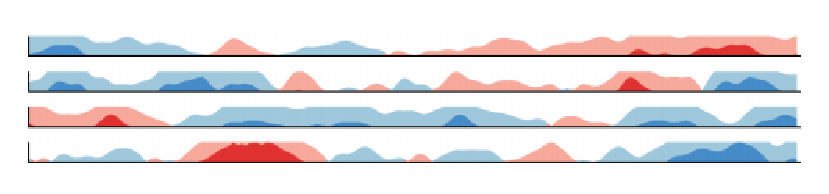
\includegraphics[width=\textwidth]{figures/eps/ts_horizongraphs.eps}
		\caption{Horizon graphs.}
		\label{fig:ts_horizon}
	\end{subfigure}
	\caption{Four possible methods for visualizing multiple time series \cite{javed2010}.}
	\label{fig:ts_compare}
\end{figure}

Multiple time series can be part of a single line chart; each series needs only to be distinguished by a color and/or line style.  However, as the number of time series on a single line chart increases, it becomes more difficult to identify an individual series.  Javed et al. evaluated the four different plotting techniques for multiple time series illustrated in Figure~\ref{fig:ts_compare} \cite{javed2010}.  The first of the techniques is the ``simple line chart,'' which was Playfair's original line chart with all series plotted together.  A slight variation on that is ``small multiples,'' where each series had its own line chart though all charts share the same axis scales.  Horizon graphs, originally developed by Saito et al., wrap around a baseline in two color tones to save space \cite{saitoTwoTone}.  Lastly, braided graphs feature all series on one chart with the coloring under the curves alternating as series intersect each other.  The user evaluation by Javed et al. revealed that a simple line graph with all time series on one plot or a single graph for each time series is better suited to a variety of tasks than a horizon graph or a braided graph.  They also found that users complete tasks more correctly when there is more display space allocated to the graphs.  They did not recommend using a higher number of simultaneous time series---their study used eight at the most---because it also leads to a decline in correctness of task completion.

\begin{figure}
	\centering
	\begin{subfigure}[b]{0.45\textwidth}
		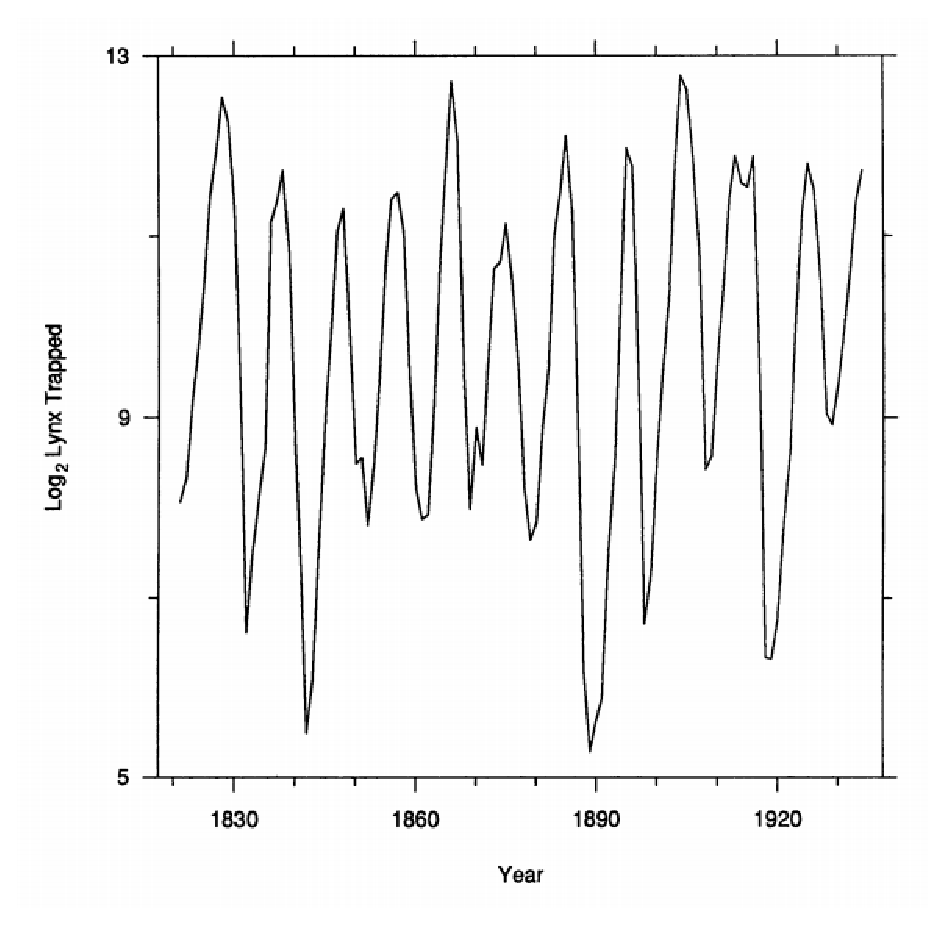
\includegraphics[width=\textwidth]{figures/eps/ratioBad.eps}
		\caption{Shape parameter of 1.0.}
		\label{fig:ratioBad}
	\end{subfigure}	
	\begin{subfigure}[b]{0.45\textwidth}
		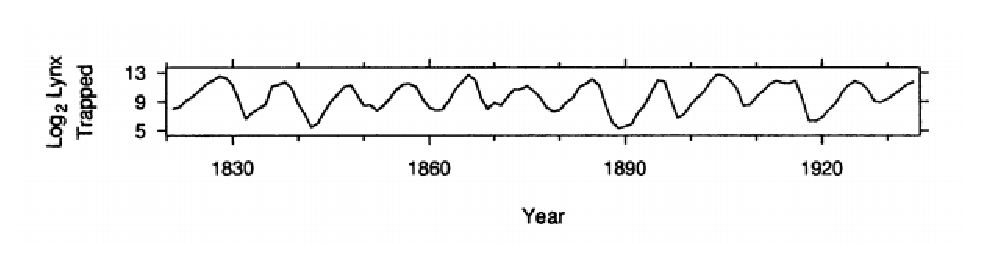
\includegraphics[width=\textwidth]{figures/eps/ratioGood.eps}
		\caption{Shape parameter of 0.074.}
		\label{fig:ratioGood}
	\end{subfigure}
	\caption{Two effect of chart shape on Canadian lynx data \cite{cleveland1988}.}
	\label{fig:ratio}
\end{figure}

Some line charts are more effective at conveying the nature of the data than others because of the way different drawing techniques affect interpretability.  Cleveland et al. found the shape of a line chart---defined as the height of the chart divided by the width of the chart---to be a critical factor \cite{cleveland1988}.   Shape of the chart directly impacts the slopes of line segments, which viewers interpret in order to understand the dependence of the $y$ variable on the $x$ variable.  Figure~\ref{fig:ratioBad}, a time series of Canadian lynx trapping data, features a shape of 1.0 and seems to imply rapid increases and decreases in the population.  On the other hand, Figure~\ref{fig:ratioGood} has a shape of 0.074 and shows more clearly that the population rises somewhat steadily and declines somewhat rapidly, which Figure~\ref{fig:ratioBad} failed to show.  Their user evaluation found that judgment of two slopes is influenced by the orientation mid-angle, defined as the average of the minimum slope orientation and the maximum slope orientation.  They proposed line chart shape should be selected such that orientations are as close to $\pm 45 ^{\circ}$ as is possible, like in Figure~\ref{fig:ratioGood}.

\begin{figure}
\centering
	\begin{subfigure}[b]{0.45\textwidth}
		\centering
		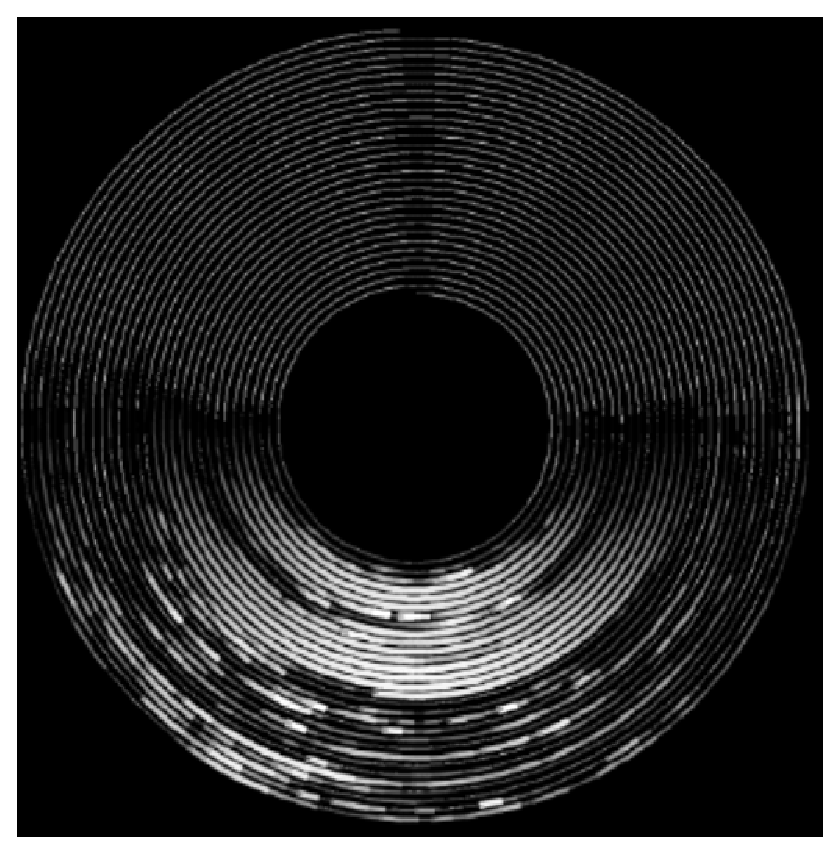
\includegraphics[height=5cm]{figures/eps/spiral.eps}
		\caption{Spiral time series.}
		\label{fig:altSpiral}
	\end{subfigure}	
	\begin{subfigure}[b]{0.45\textwidth}
		\centering
		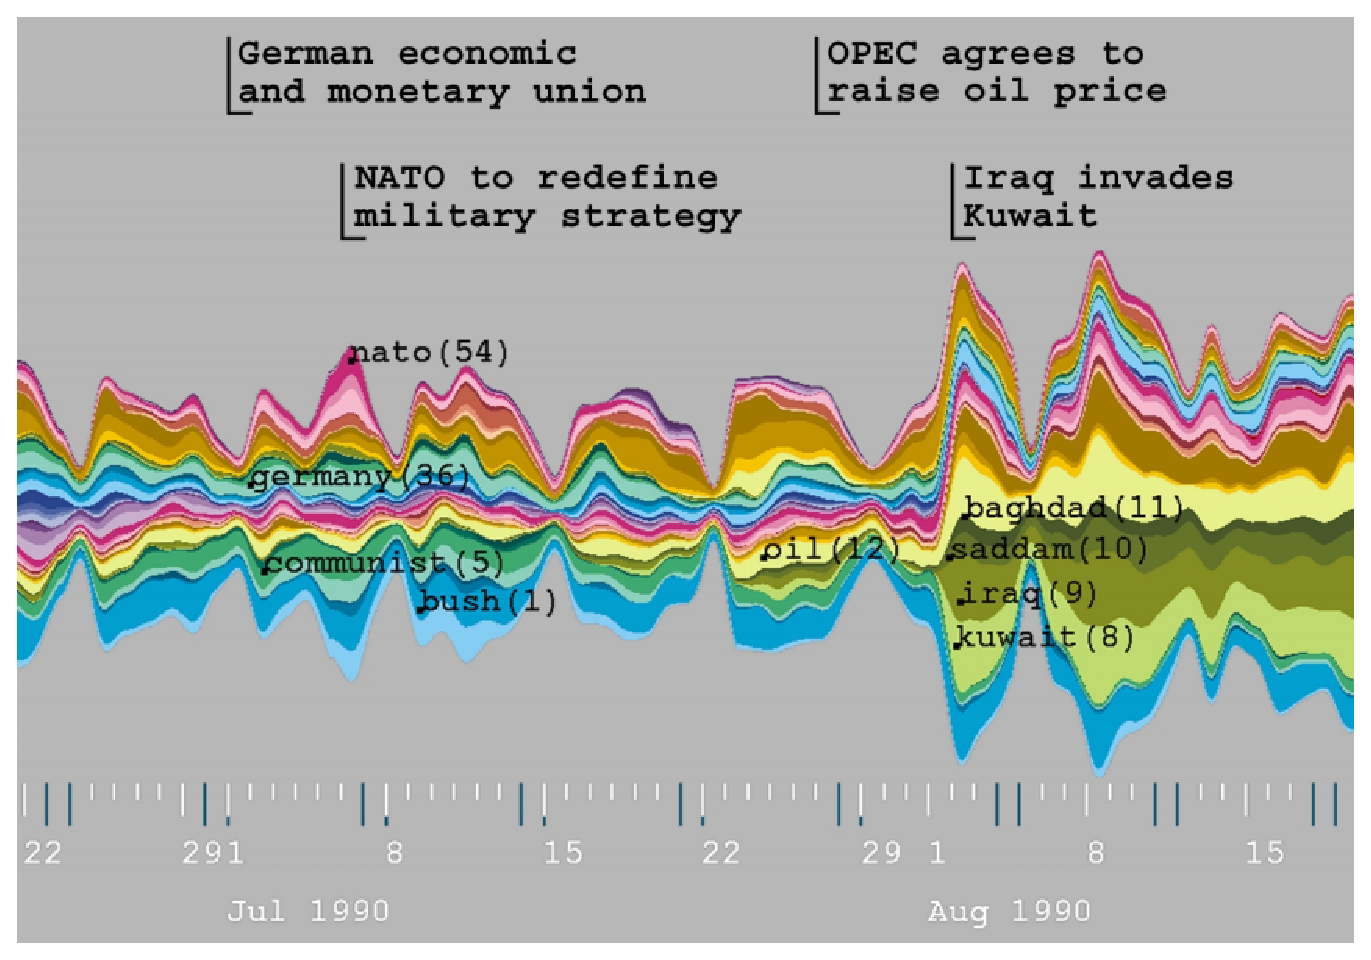
\includegraphics[height=5cm]{figures/eps/themeriver.eps}
		\caption{ThemeRiver time series.}
		\label{fig:altThemeriver}
	\end{subfigure}
	\caption{Two alternative time series visualizations.}
	\label{fig:tsAlternatives}
\end{figure}

\subsubsection{Alternatives}

There are many alternatives to and variations of Playfair's original time series.  One example is Weber et al.'s spiral time series, seen in Figure~\ref{fig:altSpiral} \cite{weber2001}.  The spiral time series was designed for cyclic data.  Cycles are emphasized in a properly-parameterized spiral visualization, however it may be difficult to describe periodic behavior in unknown datasets or determine if that behavior even exists. Another example is the ThemeRiver by Havre et al, seen in Figure~\ref{fig:altThemeriver} \cite{havre2000}.  Each ``current'' in the ThemeRiver represents an entity or subject and must be of a distinctive color.  Positioning along the y-axis is meaningless, instead the abundance of the entity or subject over time is indicated by the width of the current. 

\subsection{Networks}

The input parameters to the MS-PROD model includes predation and competition matrices.  These are relationships which may be better understood if incorporated into the visualization. Relationships are often visualized through a node-link diagram, which typically represents entities as nodes and links as relationships between the nodes they connect.  There are many types of node-link diagrams used for illustrating networks; those which are relevant to our research are discussed in the following sections.

\subsubsection{Force-Directed Layouts}

\begin{figure}[h]
	\centering
	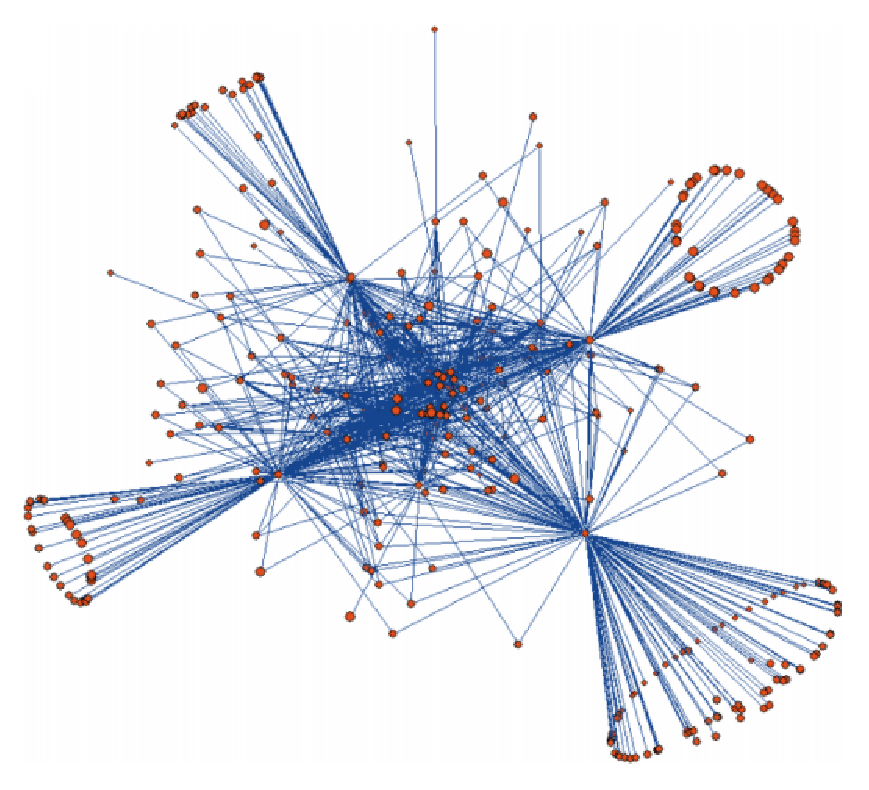
\includegraphics[width=0.85\textwidth]{figures/eps/gaichas.eps}
	\caption{A force-directed visualization of a food web of Gulf of Alaska data \cite{gaichas2008}.}
	\label{fig:gaichas}
\end{figure}

%\begin{figure}[h]
%	\centering
%	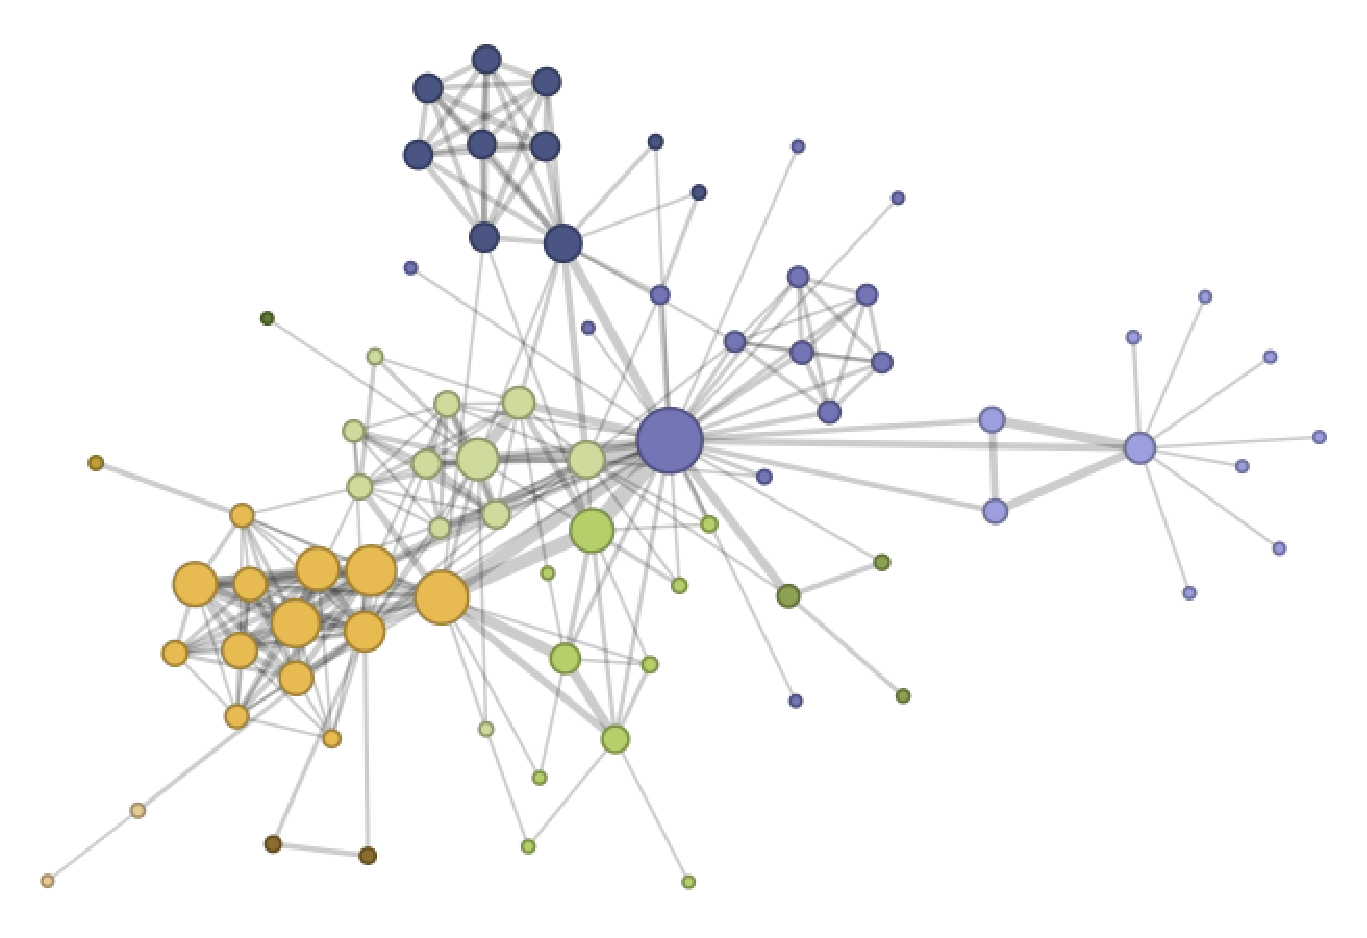
\includegraphics[width=8cm]{figures/eps/force.eps}
%	\caption{A force-directed node-link diagram \cite{Knuth:1993:SGP:164984}.}
%	\label{fig:forcedirected}
%\end{figure}

One option for showing fish species interactions would be to use a force-directed layout as Gaichas and Francis did, seen in Figure~\ref{fig:gaichas} \cite{gaichas2008}.  Here, the nodes represent an individual species in the Gulf of Alaska, while the links represent a predator-prey interaction.  In a force-directed layout, nodes repel each other, while related nodes become pulled toward each other by links \cite{heer2010}.  The result is an aesthetically pleasing layout where there are relatively few link crossings and links are of approximately similar length.  The color of the node can be used to indicate group membership, while the size can represent the magnitude of some property of the node.  Likewise, the drawing style of the link can be varied to encode different types of relationships. 

\subsubsection{Arc Diagrams}

\begin{figure}[h]
	\centering
	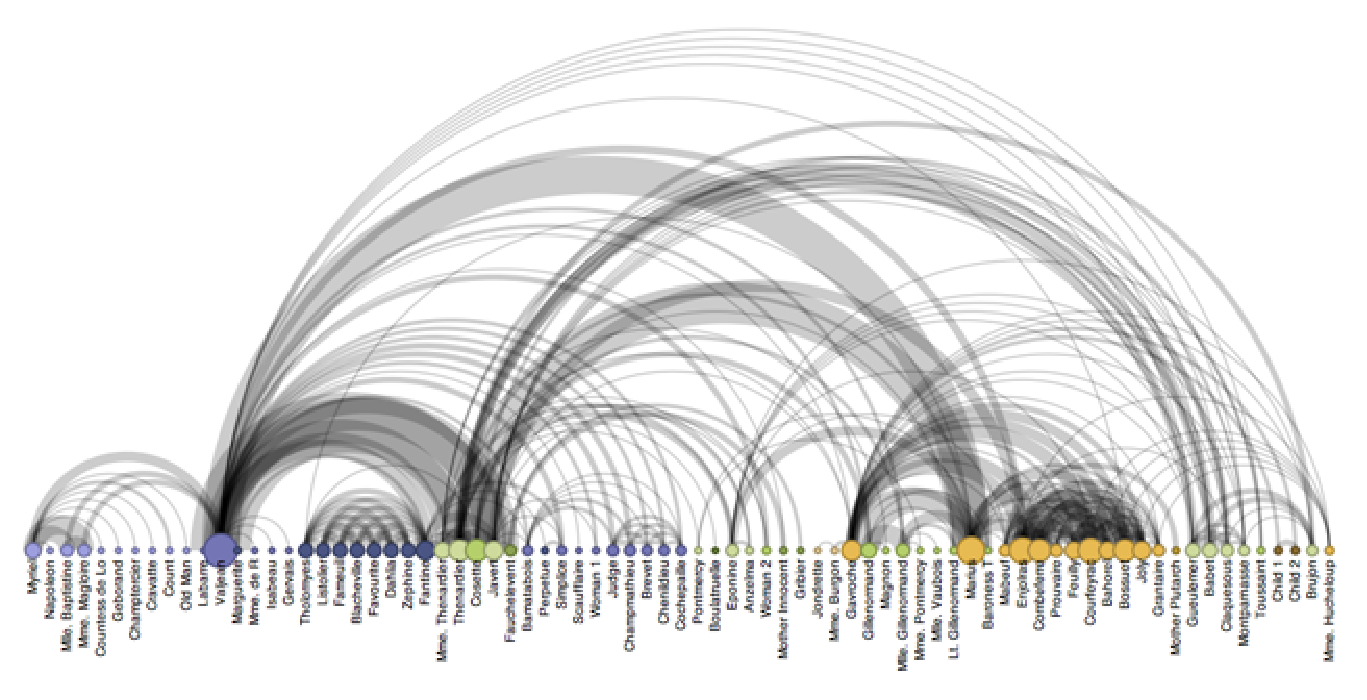
\includegraphics[width=0.95\textwidth]{figures/eps/arcdiagram.eps}
	\caption{Knuth's arc diagram of \textit{Les Mis\'erables} characters \cite{knuth1993}.}
	\label{fig:arcdiagram}
\end{figure}

An alternative for force-directed layout is an arc diagram.  The name arc diagram was coined by Wattenberg \cite{wattenberg2002}, though they were invented earlier.  Knuth used arc diagrams to illustrate interaction of characters in Victor Hugo's novel \textit{Les} \textit{Mis\'erables}, seen in Figure~\ref{fig:arcdiagram} \cite{knuth1993}.  Each character is represented with a circular node, where size indicates the number of appearances in the novel.  The nodes are arranged linearly, colored and ordered according to clusters of characters that appear together frequently.  Semi-transparent arcs are drawn between the characters which appear in the same chapter, with the thickness of the arc representing the number of such appearances.  While the arc diagram may fail to properly depict the structure of a network, Heer et al. point out it is advantageous because the one-dimensionality allows for other features to be easily displayed near the nodes \cite{heer2010}, such as text labels.

\subsubsection{Directed Edges}

\begin{figure}[h]
	\centering
	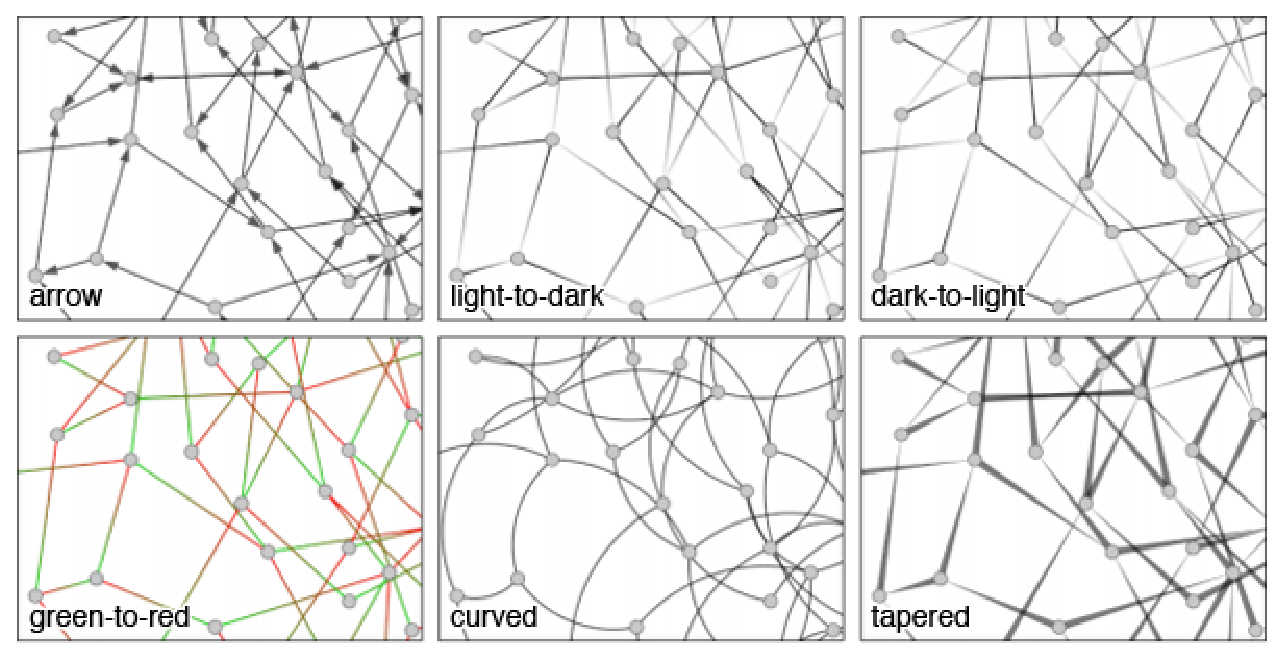
\includegraphics[width=0.95\textwidth]{figures/eps/directedEdges.eps}
	\caption{Different types of directed edges \cite{holten2009}.}
	\label{fig:directedEdges}
\end{figure}

Relationships in a network may be directional, such as the predator-prey relationship.  In a visualization of such a network, the direction of the edges must be encoded so these relationships can be understood.  Holten and van Wijk studied the effectiveness of different techniques for indicating directionality of edges in a graph, seen in Figure~\ref{fig:directedEdges} \cite{holten2009}.  The traditional arrowhead was found to perform poorly, while tapered edges performed best.  As for an intensity-based direction cue, a dark-to-light representation was found to be clearer than light-to-dark.

\subsubsection{Matrix Representations}

\begin{figure}[h]
	\centering
	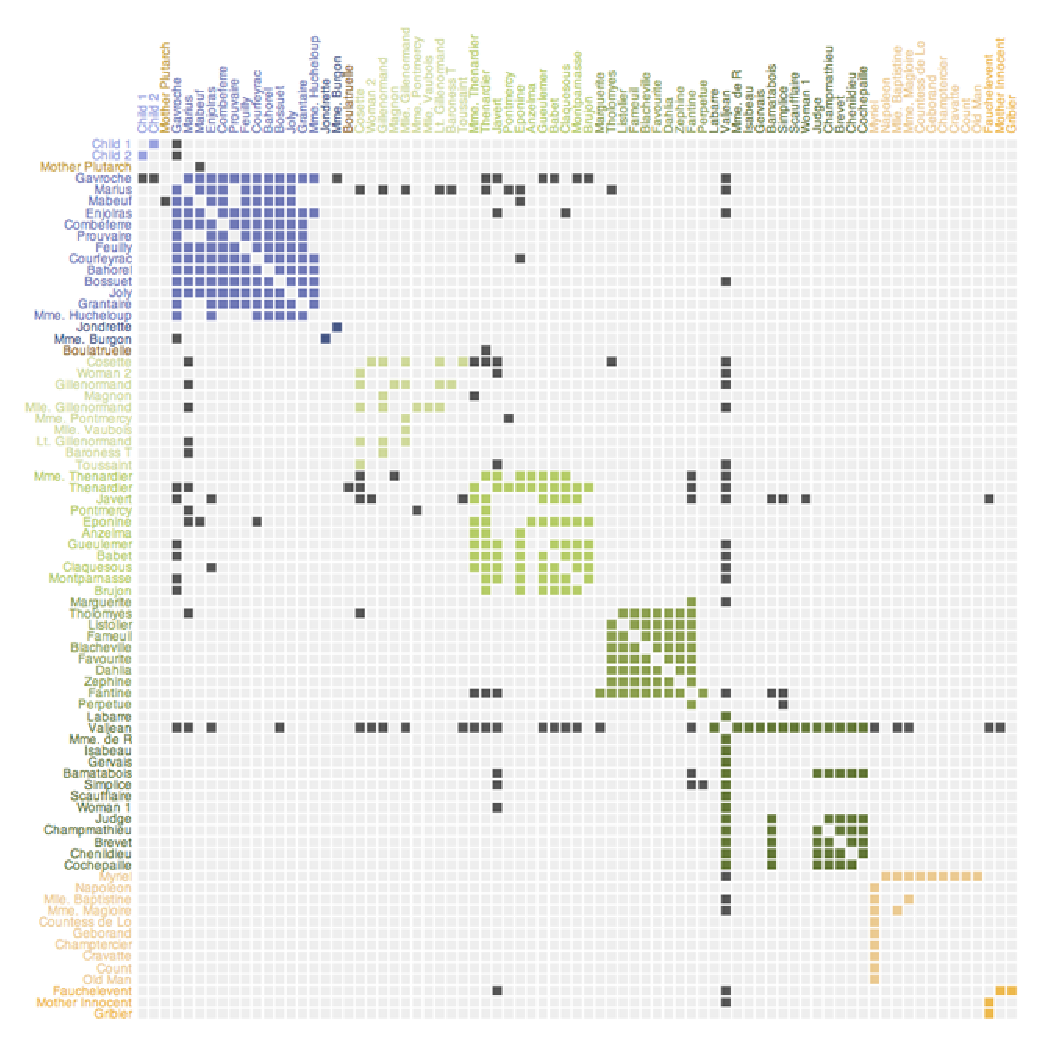
\includegraphics[width=0.95\textwidth]{figures/eps/matrix.eps}
	\caption{A matrix-based visualization of an adjacency matrix \cite{knuth1993}.}
	\label{fig:matrix}
\end{figure}

Node-link diagrams can have occlusion problems when they are highly-connected, so a matrix-based representation of a network is a possible alternative \cite{heer2010}.  In many cases, networks are stored as an adjacency matrix, so all that needs to be done is visualize that matrix as a grid, where the cell at the $i$th row and the $j$th column represents the relationship from entity $i$ to entity $j$.  Figure~\ref{fig:matrix} shows Knuth's visualization of \textit{Les} \textit{Mis\'erables} characters in matrix-form \cite{knuth1993}.  The color of the cell indicates the presence or type of a relationship, with some neutral color indicating the lack of a relationship.  Ghoniem et al. showed that a matrix-based view is suitable for large or dense networks for tasks that involve finding or counting links or nodes \cite{ghoniem2004}.  With proper ordering of the rows and columns, the structure of the network can be effectively displayed, however path-finding tasks may be difficult.

\subsection{Causality}

Gamble and Link found that both inter-species relationships and harvesting by humans can contribute to changes in species biomass according to their MS-PROD model \cite{gamble2009}.  For example, a increase in biomass for one species could possibly hinder growth for another species.  This is a type of cause and effect relationship, therefore it is necessary to consider the various techniques for representing causality in a network, especially in an interactive context.

\begin{figure}
\centering
	\begin{subfigure}[b]{0.3\textwidth}
		\centering
		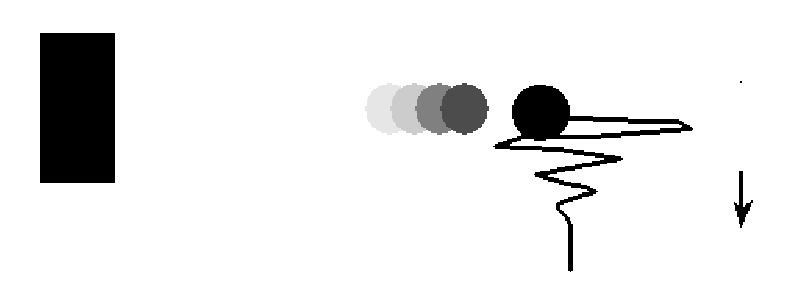
\includegraphics[width=0.95\textwidth]{figures/eps/vcv_pinball.eps}
		\caption{Pinball.}
		\label{fig:vcvPinball}
	\end{subfigure}	
	\begin{subfigure}[b]{0.3\textwidth}
		\centering
		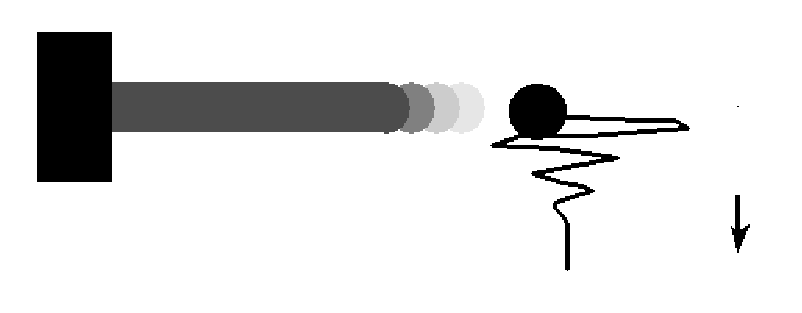
\includegraphics[width=0.95\textwidth]{figures/eps/vcv_prod.eps}
		\caption{Prod.}
		\label{fig:vcvProd}
	\end{subfigure}
	\begin{subfigure}[b]{0.3\textwidth}
		\centering
		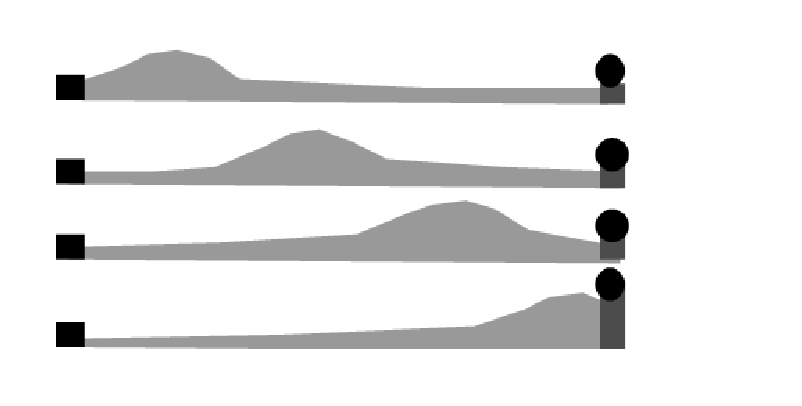
\includegraphics[width=0.95\textwidth]{figures/eps/vcv_wave.eps}
		\caption{Wave.}
		\label{fig:vcvWave}
	\end{subfigure}
	\caption{Three metaphors for conveying causality \cite{ware1999}.}
	\label{fig:vcv}
\end{figure}

Michotte and Thin\'es suggested that viewers infer causality after viewing an object being set into motion after being struck by another object \cite{michotte1963}.  This served as a basis for Ware et al.'s visual causality vector (VCV), which communicates causal relationships between two nodes in a network visualization \cite{ware1999}.  They studied how several animated metaphors---shown in Figure~\ref{fig:vcv}---and different timing rules for a VCV affect the perception of causality.  Their evaluation showed that temporal synchrony between the animation of the metaphor and the changes in the recipient node is more critical than the type of metaphor for showing causal relationships.  Ware later revisited this work in the context of multi-touch screens to convey causal effect enhancements, causal effect reductions, and causal blocking effects using colored pulses \cite{ware2013}.  The user evaluation conducted by Ware showed that causal blocking effects and positive enhancements were well understood with this design, while negative causal effects were less reliably judged.  Still, these methods were recommended for showing simple causal relationships.

\begin{figure}
\centering
	\begin{subfigure}[b]{0.47\textwidth}
		\centering
		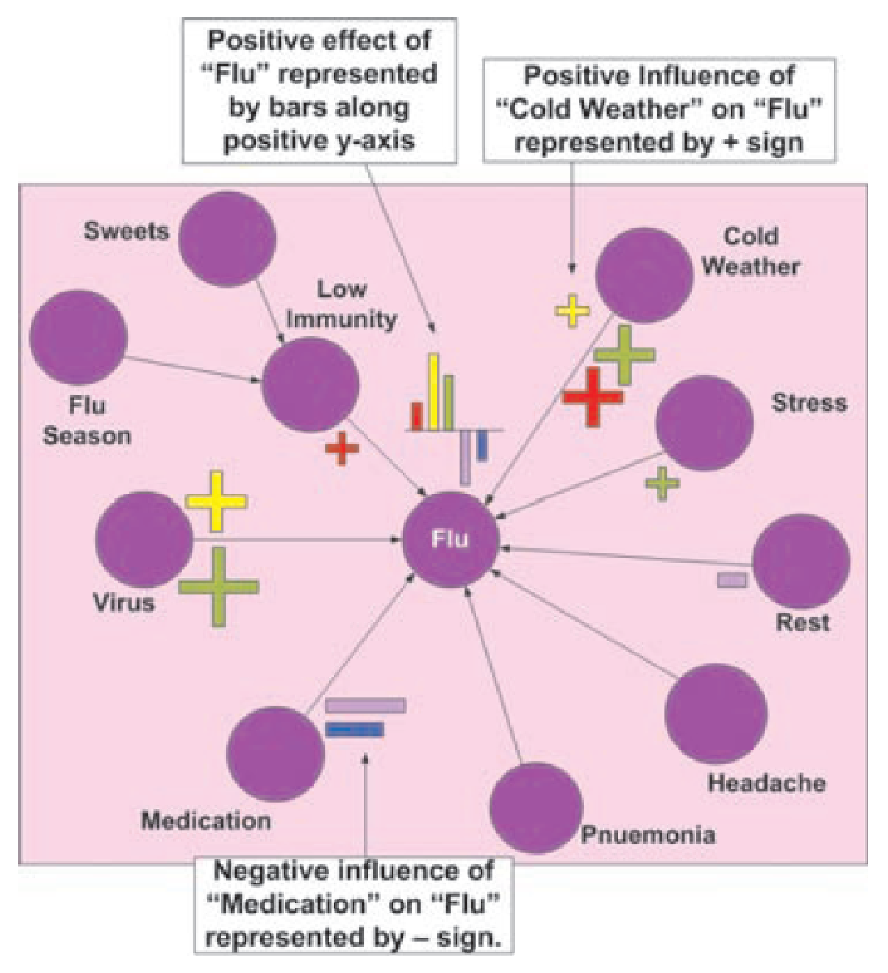
\includegraphics[width=0.95\textwidth]{figures/eps/kadaba_static.eps}
		\caption{Static.}
		\label{fig:kadabaStatic}
	\end{subfigure}	
	\begin{subfigure}[b]{0.47\textwidth}
		\centering
		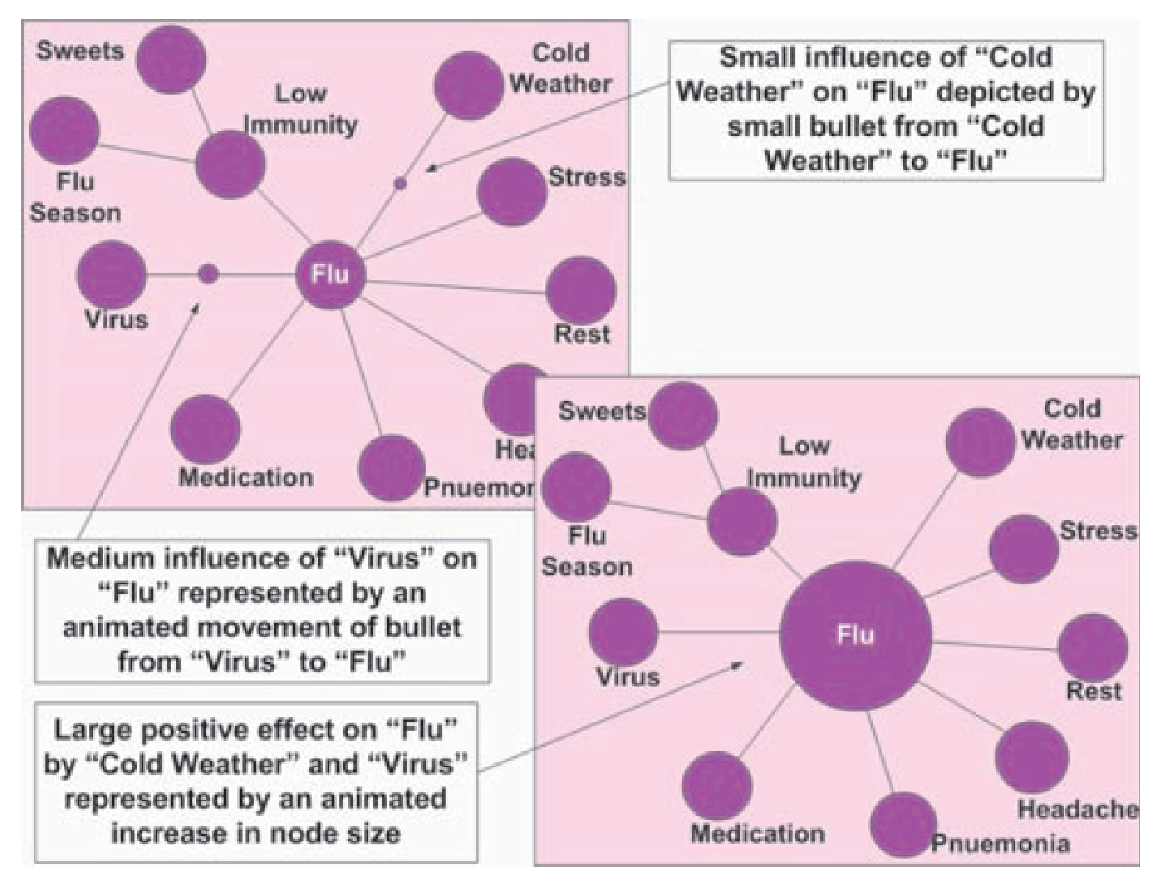
\includegraphics[width=0.95\textwidth]{figures/eps/kadaba_animated.eps}
		\caption{Animated.}
		\label{fig:kadabaAnimated}
	\end{subfigure}
	\caption{Two alternatives for visualizing causal influences \cite{kadaba2007}.}
	\label{fig:kadaba}
\end{figure}

Kadaba et al.\ expanded upon Ware et al.'s VCV work to compare between static and animated causal visualizations \cite{kadaba2007}.  In their static design, positive influences were indicated with a plus sign ($+$) glyph and negative influences were indicated with a minus sign ($-$) glyph attached to the link between two entities in the network, as in Figure~\ref{fig:kadabaStatic}.  The size of the glyph represented the magnitude of the influence on the recipient node and glyphs of the same color described a multiplication effect on the recipient.   Their animated design featured bullets traveling along the links toward the recipient node to indicate causal influences, shown in Figure~\ref{fig:kadabaAnimated}.  As a bullet hit the recipient node, the size of the recipient node changed.  They found that subjects can interpret animated and static representations equally accurately, but subjects formed responses slightly quicker with animated representations.

\subsection{Uncertainty}

\begin{figure}
\centering
	\begin{subfigure}[b]{0.45\textwidth}
		\centering
		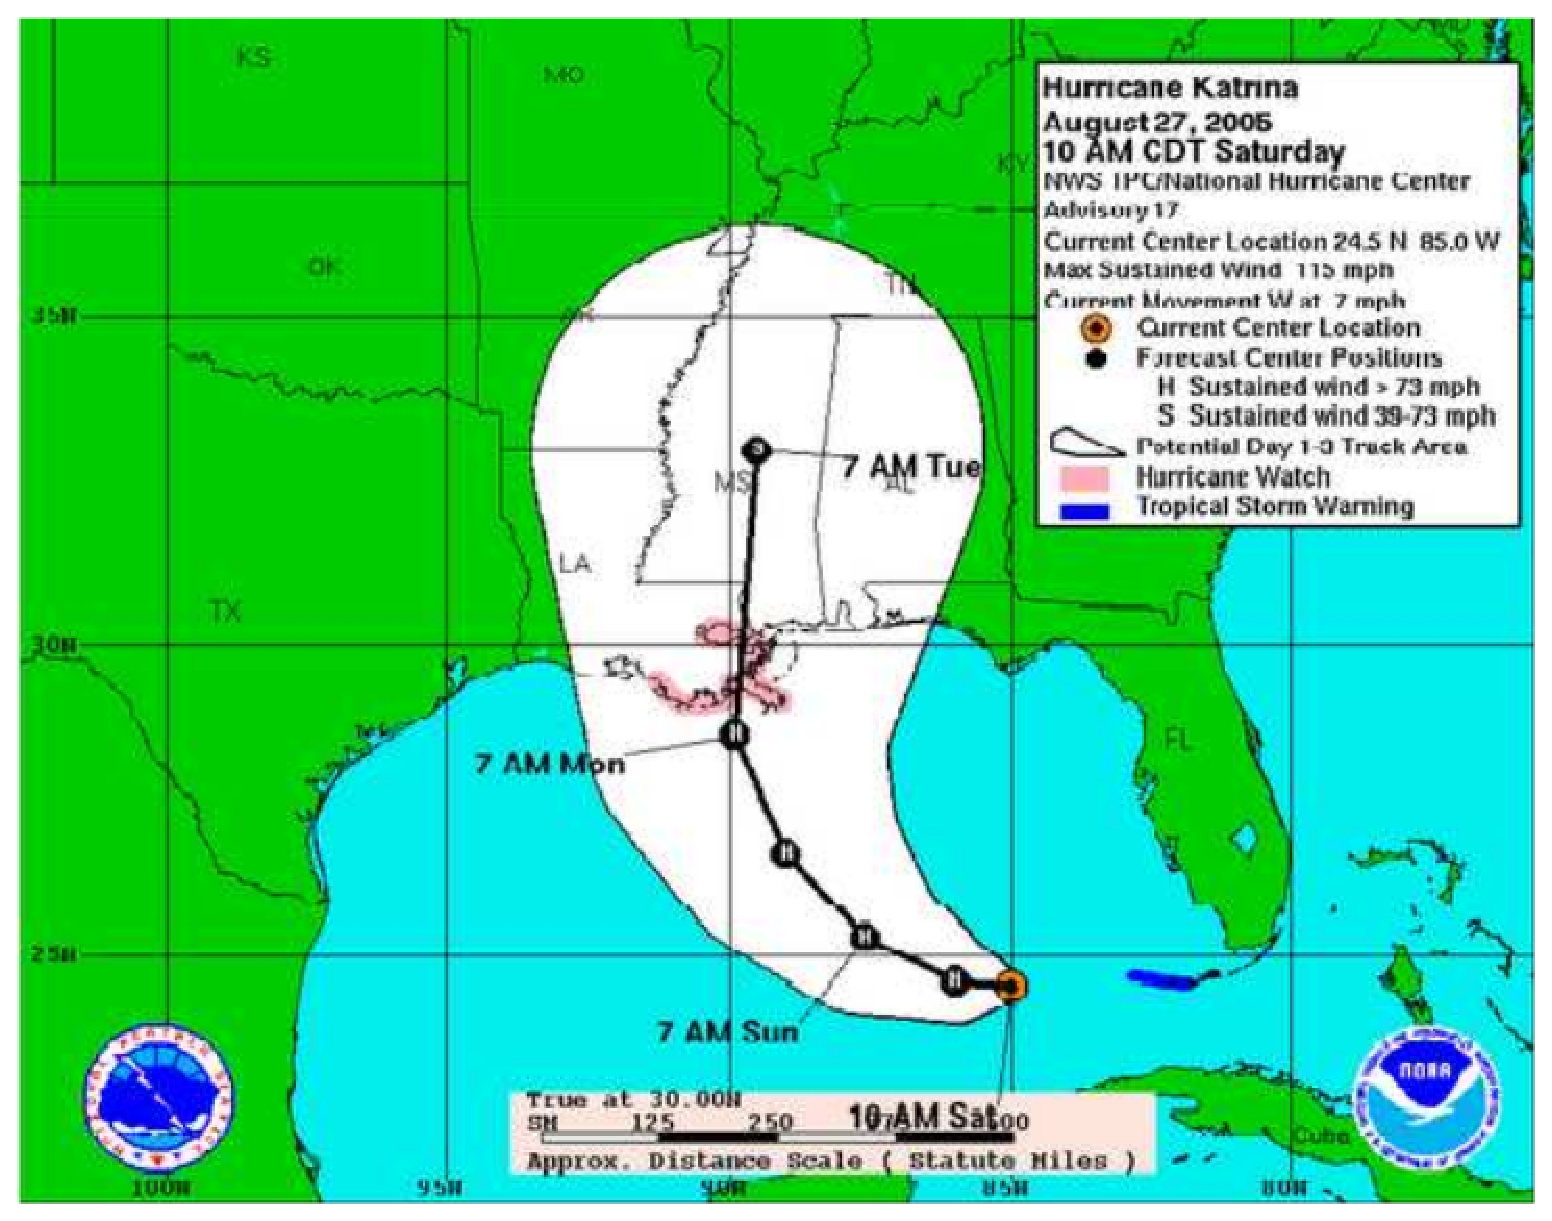
\includegraphics[height=4.5cm]{figures/eps/uncertainty_cone.eps}
		\caption{Error cone.}
		\label{fig:uncertaintyCone}
	\end{subfigure}	
	\begin{subfigure}[b]{0.45\textwidth}
		\centering
		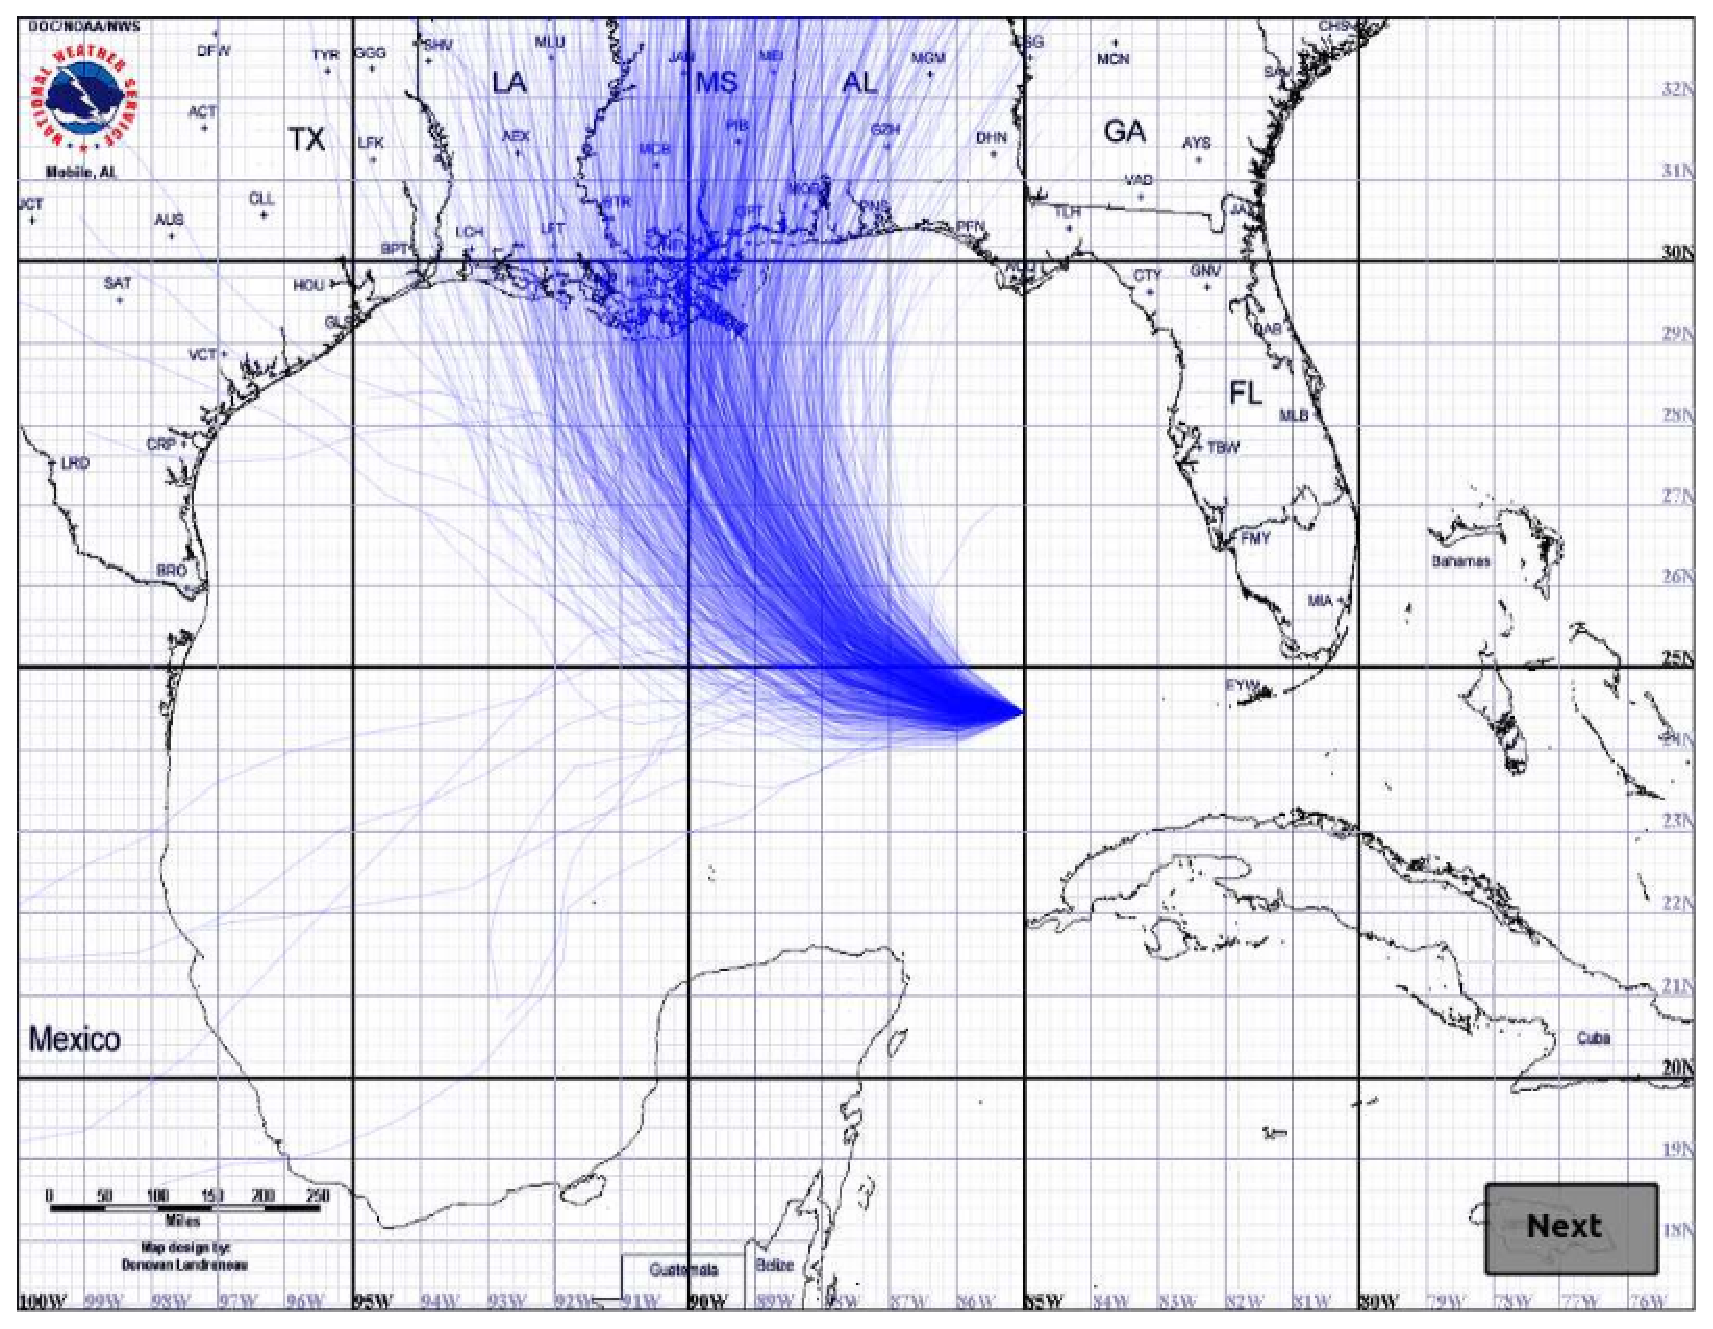
\includegraphics[height=4.5cm]{figures/eps/uncertainty_house.eps}
		\caption{Cox et al.'s method.}
		\label{fig:uncertaintyHouse}
	\end{subfigure}
	\caption{Two visualizations of uncertainty for a hurricane advisory \cite{cox2013}.}
	\label{fig:uncertaintyAlternatives}
\end{figure}

A model is a simplification of reality, therefore it is common for its output to be regarded with some uncertainty.  To clarify, \textit{error} describes inaccuracies when the correct answer is known, while \textit{uncertainty} describes inaccuracies when the answer is unknown \cite{hunter1993}.  Therefore, model output is best understood as a range of expected values which is likely to contain the true value.  According to Potter et al., scientific data can be considered to be incomplete without representations of uncertainty \cite{potter2010}, so we have investigated some different portrayals of uncertainty.
%Uncertainty can arise at several stages---the conceptualization of the model, the collection of the model input, or due to data transformations \cite{}.

Cox et al. explored methods for depicting uncertainty for hurricane advisories \cite{cox2013}.  The traditional error cone, as in Figure~\ref{fig:uncertaintyCone}, is used by NOAA's National Hurricane Center, but it can be poorly understood by the average citizen.  They produced their own creation, as in Figure~\ref{fig:uncertaintyHouse}, where many possible hurricane tracks are drawn to describe the range of possible outcomes.  Their user evaluation found that neither method was significantly better than the other for all cases, but a qualitative analysis showed that nearly all users prefer their new method over the error cone.

\section{Understanding Models}

Users studying models can benefit from the aid of a visualization, because patterns and trends may be difficult---if not impossible---to discern from only a table of numerical values.  The learning process can be even further enhanced through interaction with the model.  If interactivity is supported by the visualization, then users can adjust parameter values, perceive a change (or perhaps no change) in the results, and begin to understand the degree of influence different parameters possess.

\subsection{Spreadsheet Programs}

\begin{figure}
\centering
	\begin{subfigure}[b]{0.4\textwidth}
		\centering
		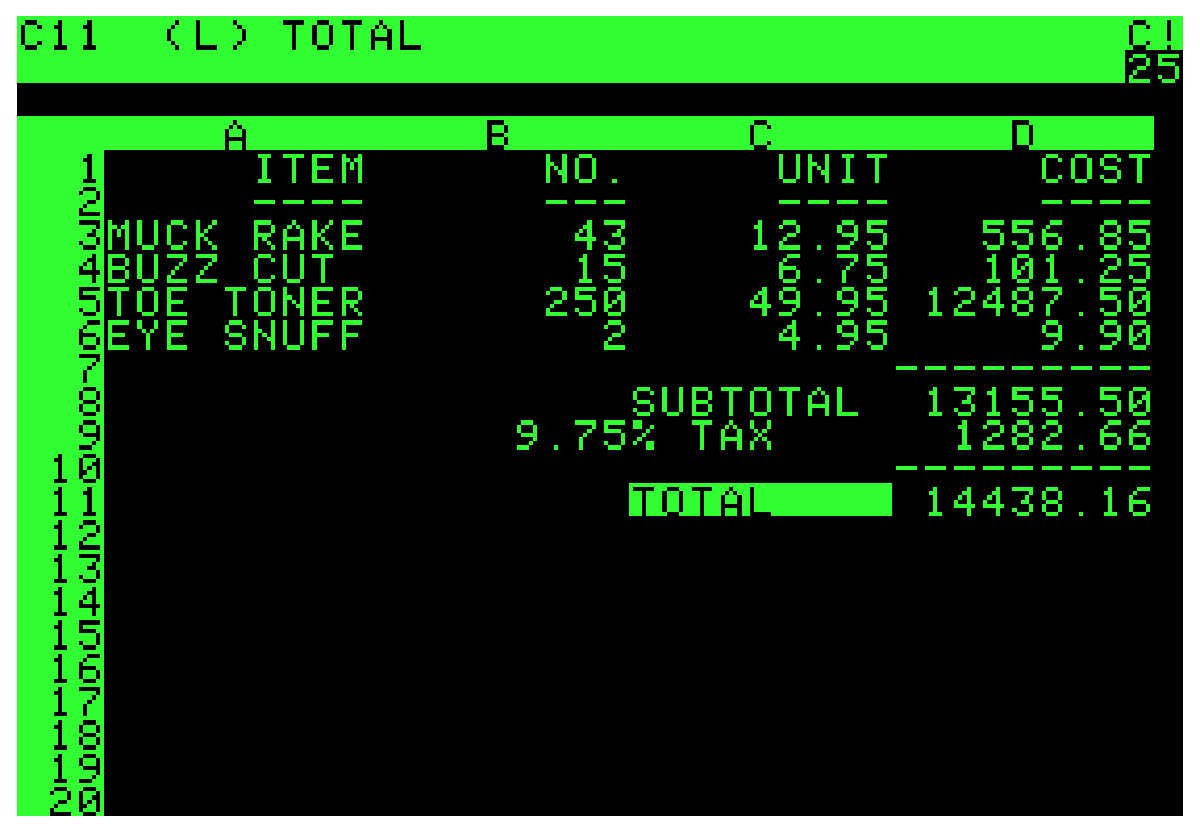
\includegraphics[height=4cm]{figures/eps/visicalc.eps}
		\caption{A screenshot of VisiCalc (GNU General Public License).}
		\label{fig:visicalc}
	\end{subfigure}	
	\begin{subfigure}[b]{0.4\textwidth}
		\centering
		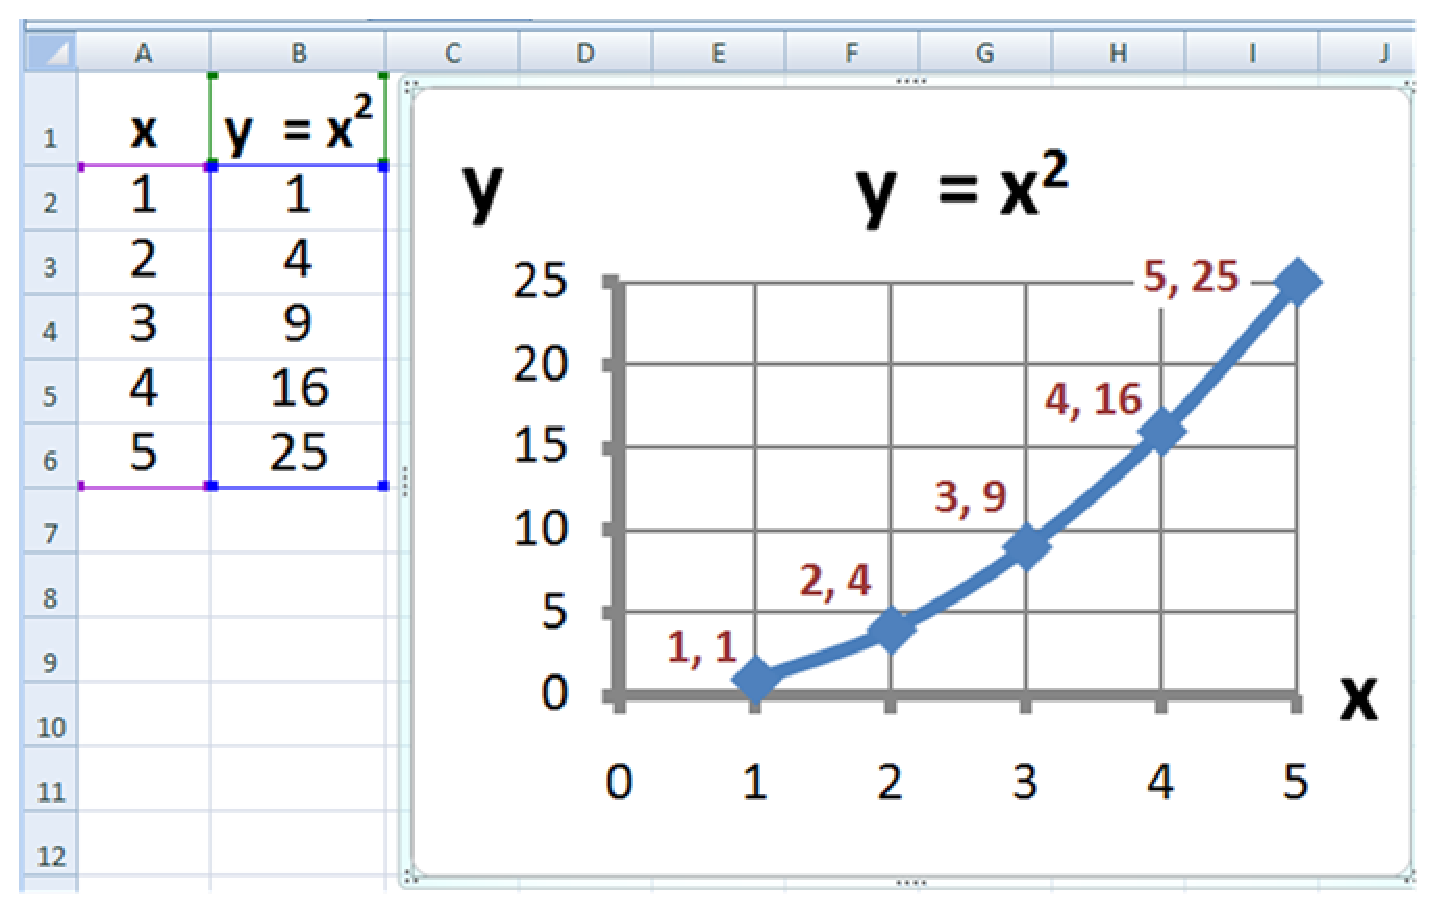
\includegraphics[height=4cm]{figures/eps/excel.eps}
		\caption{A chart made using Microsoft Excel (public domain).}
		\label{fig:excel}
	\end{subfigure}
	\caption{Two examples of spreadsheet applications.}
	\label{fig:spreadsheets}
\end{figure}

VisiCalc was a very early example of software assisting the understanding of models \cite{grad2007}.  As a business student, Bricklin wished there was a faster way to change the input or fix mistakes when working out financial models by hand \cite{bricklin1999}.  To address this, he worked with Frankston to develop VisiCalc, seen in Figure~\ref{fig:visicalc}.  As the world's first electronic spreadsheet, VisiCalc consisted of rows and columns containing either text, numerical values, or formulas.  Result cells were instantly updated according to changed inputs or adjusted formulas, allowing a user to work with models in a more efficient and dynamic manner.  VisiCalc was superseded by Lotus 1-2-3, which was in turn supplanted by Microsoft Excel.  Microsoft Excel remains popular and features graphing tools which can generate charts, such as in Figure~\ref{fig:excel}.

\subsection{The Influence Explorer}

\begin{figure}[h]
	\centering
	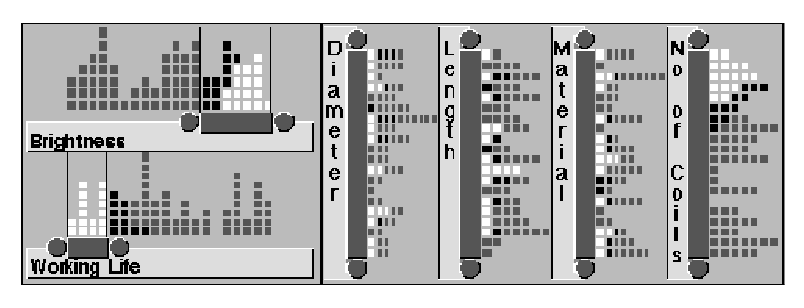
\includegraphics[width=0.95\textwidth]{figures/eps/influenceExplorer.eps}
	\caption{A screenshot of the Influence Explorer \cite{tweedie1995}.}
	\label{fig:influenceExplorer}
\end{figure}

The Influence Explorer by Tweedie et al. is a good example of a more complex interactive visualization \cite{tweedie1995}.  They developed an interface for understanding the relationships between different attributes in a design process.  Parameter values of the Influence Explorer are initially randomly selected to represent different possible items.  For each attribute, there is a histogram including each of the items.  The attribute ranges are controlled by sliders.  When the user adjusts the slider of a given attribute, all items that are within that range are highlighted on all of the histograms.  Figure~\ref{fig:influenceExplorer} is a screenshot of the Influence Explorer being used to test the performance of different light bulb designs; white indicates the design passed, black it failed one specification, and grey it failed two specifications.  In a user evaluation, industrial designers found the ability to interactively explore the effects of different parameter ranges to be valuable.

\subsection{Vensim}

\begin{figure}[h]
	\centering
	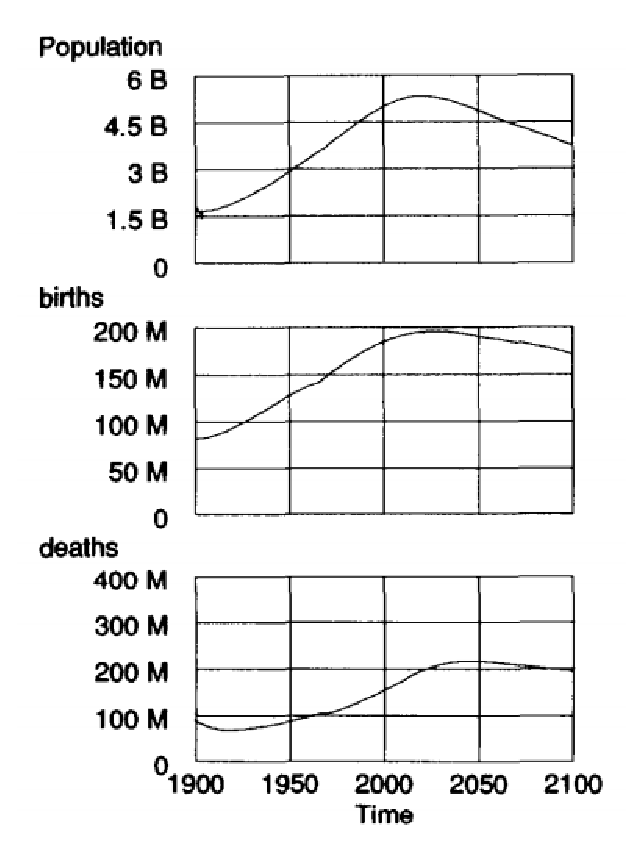
\includegraphics[width=6cm]{figures/eps/vensim.eps}
	\caption{A screenshot of the strip graphs in Vensim \cite{eberlein1992}.}
	\label{fig:vensim}
\end{figure}

Eberlein and Peterson recognized that both unskilled and skilled model users have the same need: to quickly obtain a thorough understanding of a model and its implications \cite{eberlein1992}.  This motivated their development of Vensim, which is a commercial tool for visualizing and analyzing simulation results.  Vensim allows users to run a model under different conditions with a simple mouse click, enabling the user to learn the effects of different actions with ease.  Various features enhance this learning process---e.g., ``causal tracing'' strip graphs, shown in Figure~\ref{fig:vensim}.  Rather than simply seeing a chart of the projected population, a user exploring the causal tracing feature can begin to understand the various components that contributed to the population simulations---births and deaths---by seeing each component on its own chart.  A major emphasis of Eberlein and Peterson is that the same visualization tool can and should be used for both the development and teaching phases of a model, especially since those phases may not be discrete.

\chapter{Requirements and Design}

%The bulk of the design and implementation of an interactive interface to the MS-PROD model has been completed.  However, this is not a final design; in many cases, several design alternatives have been implemented and await the evaluation study prior to final implementation.  These alternatives are described below.

The motivation of this research is to provide an interactive interface to the NOAA MS-PROD model so as to help fishermen, fisheries managers, and other stakeholders understand the implications of decisions, such as changing catch quotas for particular kinds of fishing activity---e.g., bottom trawling versus mid-water trawling.  We planned our interactive interface with the intent that users would gain insight into:

\begin{itemize}
	\item \textbf{Implications of the model:}  E.g., how do two different sets of fishing effort values affect the biomass predictions of the ten species?
	\item \textbf{The model itself:}  E.g., why does the abundance of one species increase when another species is caught? 
\end{itemize} 

To accomplish this goal, we determined our interactive interface of the MS-PROD model would need to visualize:

\begin{itemize}
	\item The predicted biomass over time,
	\item Changes in predicted biomass as a result of changes in fishing effort,
	\item Causal relationships which help to explain indirect or unintuitive results,
	\item Uncertainty of the model
\end{itemize} 

Since setting fishing quotas is the only action fishery managers can take, we determined that the only interaction available to users would be to adjust the fishing effort level; all other model parameters are not modifiable once the model and its visualization are running.  This interaction is done by means of a set of sliders with the goal of allowing the user to immediately see the impact of management decisions on fisheries.  The user adjusts sliders which represent harvest effort and watches the biomass plots change instantaneously as the model is re-run according to the new effort values.  Like Eberlein and Peterson, we aimed to turn the ``time consuming and tedious'' task of working with a model into a ``fast and fun'' interactive experience \cite{eberlein1992}.  Different views and features of the model visualization are described and discussed in the sections below.  

It is important to note that the MS-PROD model allows for different fishing effort values for each species for each year in the thirty-year period that the model produces forecasts for.  This is to reflect that fishing quotas can change from year to year.  Since there are ten species and thirty years, this means there are potentially 300 separate fishing effort values that could be set by a user.  However, it would be cluttered and confusing to have an effort slider for each of those 300 values.  Therefore, two simplifications were made.  First, fishing effort should be controlled by functional group rather than individual; the model authors requested this because it is more realistic than fishing by individual species.  Second, fishing effort for a functional group is constant across all thirty years; while this is unrealistic, it is easier to understand and perhaps, in a sustainable, ``perfect world,'' fishing quotas would not need adjusting over the years.  Thus, each slider controls the fishing effort for all thirty years for a particular functional group.

\section{Visualization of Predicted Biomass}

First and foremost, we had to decide how to display the thirty-year biomass forecast data output by the model.  Time series line charts---of both the simple line chart and small multiples varieties---were chosen because casual viewers can understand them without further instructions, as opposed to, say a horizon graph.  Another advantage to line charts is that they tend to have a reasonable amount of whitespace where additional information can be displayed, such as uncertainty or alternate forecasts. A key design issue concerned the representation of change between two forecasts; line charts provide the ability to display this change.  A number of alternatives for change were implemented and are described in the sections that follow.

\subsection{Alternative Screen Layouts}

Once it was decided that time series were most appropriate for our task, we had to choose how many individual charts should be used to display the data and how to arrange them.  Two alternative screen layouts were developed for displaying these time series on line charts: a ``four panel'' view in Figure~\ref{fig:msprod_group} and a ``small multiple'' view in Figure~\ref{fig:msprod_species}, described in further detail below.  With both views, the time series for the species are organized by functional group.  A functional group is a biological grouping of species which perform similar functions within their ecosystem---e.g., mackerel and herring are both members of the ``small pelagic'' group since they live in the water column.

There were several reasons for the decision to arrange by functional group rather than placing all time series on a single line chart.  First, harvest effort is controlled by functional group using the sliders, so it must be somehow indicated which species are part of which functional group.  With multiple time series, this can be encoded through positioning by arranging the slider of a functional group to be near the time series of that group's species.  Second, it would have been impractical to simply place all time series on a single line chart because would have been difficult to select enough distinct colors to represent each of the ten species.  Furthermore, the biomass of some species is significantly larger than others.  By scaling the $y$-axis according to the largest biomass value of all species in the entire 30-year time span, the lines representing some species would have been crowded at the bottom of the chart and seemed to be flat even when they were not.

\subsubsection{Four Panel View}

\begin{figure}[h]
	\centering
	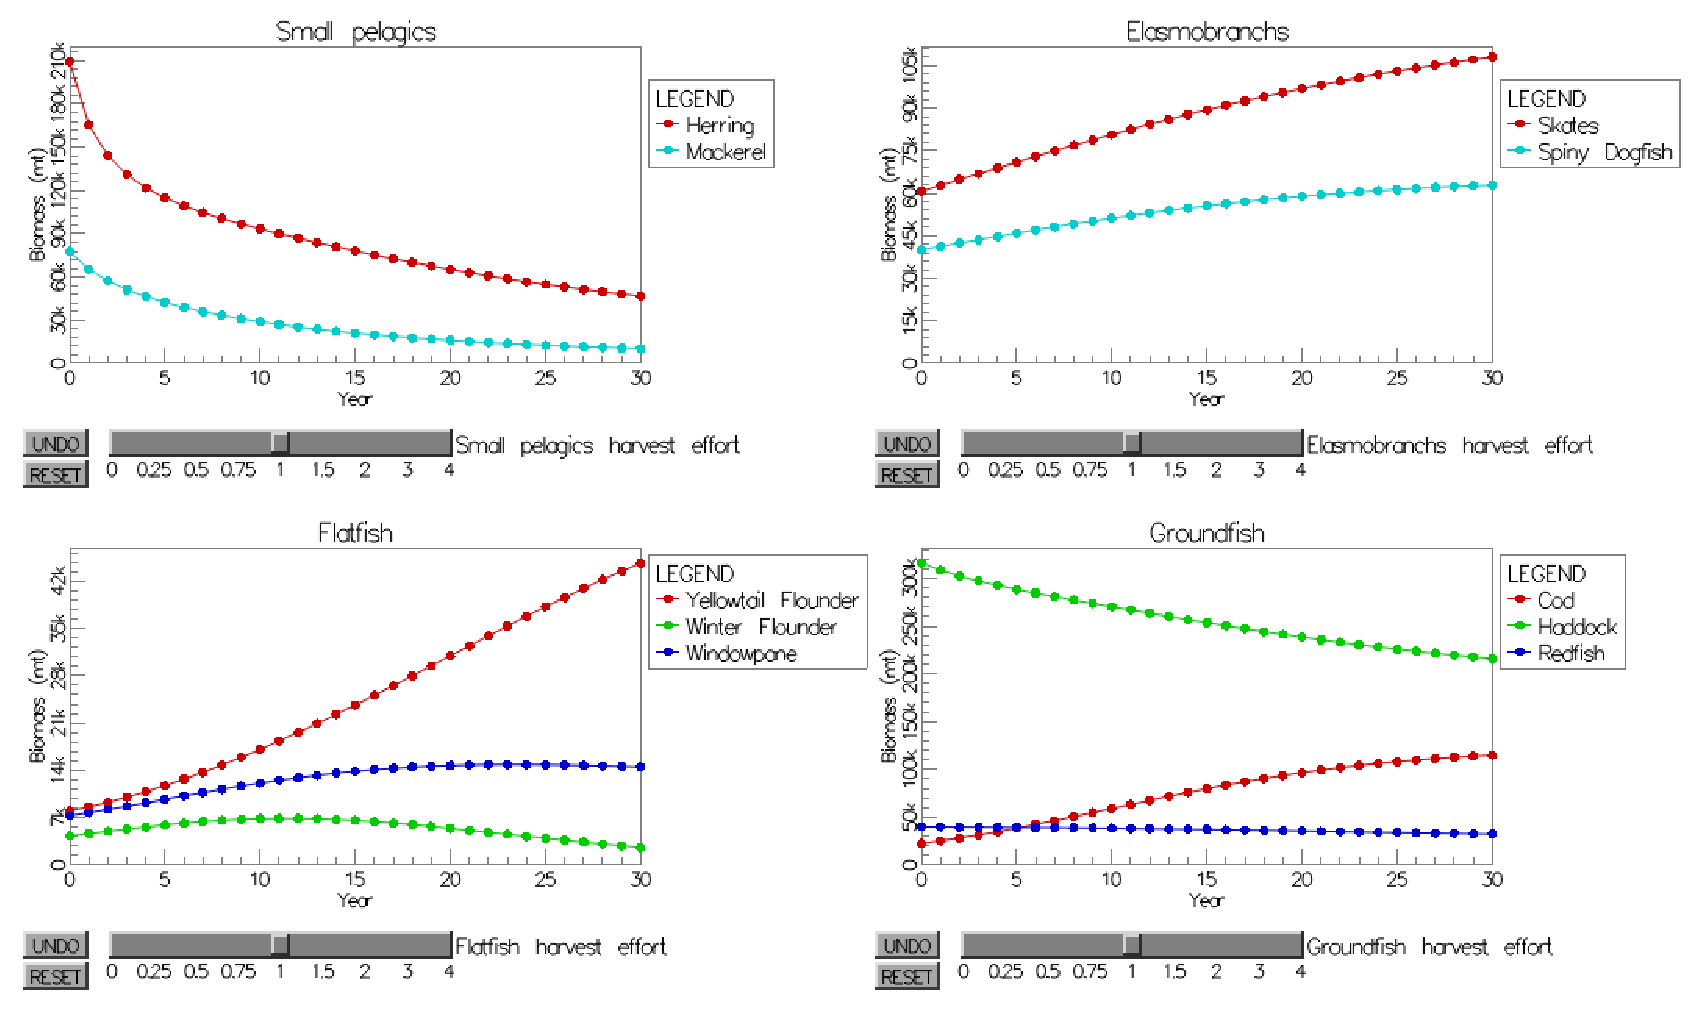
\includegraphics[width=14cm]{figures/eps/msprod_group.eps}
	\caption{The ``four panel'' view of our MS-PROD visualization.}
	\label{fig:msprod_group}
\end{figure}

It was observed that species of similar functional groups tend to have biomass values in similar numeric ranges, so a decision was made to have one line chart per functional group for displaying biomasses.  This view is called the ``four panel'' view and is shown in Figure~\ref{fig:msprod_group}.

The major advantage of this ``four panel'' view is that comparison of species within a group is easy.  For MS-PROD, there are only two or three species per functional group, so the line chart for each group tends to not suffer from occlusion problems.  Direct and indirect effects of changes in harvest effort are easily differentiated with the ``four panel'' approach---e.g., if the user adjusts the effort slider only for elasmobranchs, yet sees the biomasses change on the groundfish chart, then the user can begin to understand there is some kind of relationship between elasmobranchs and groundfish.

\subsubsection{Small Multiples View}

\begin{figure}[h]
	\centering
	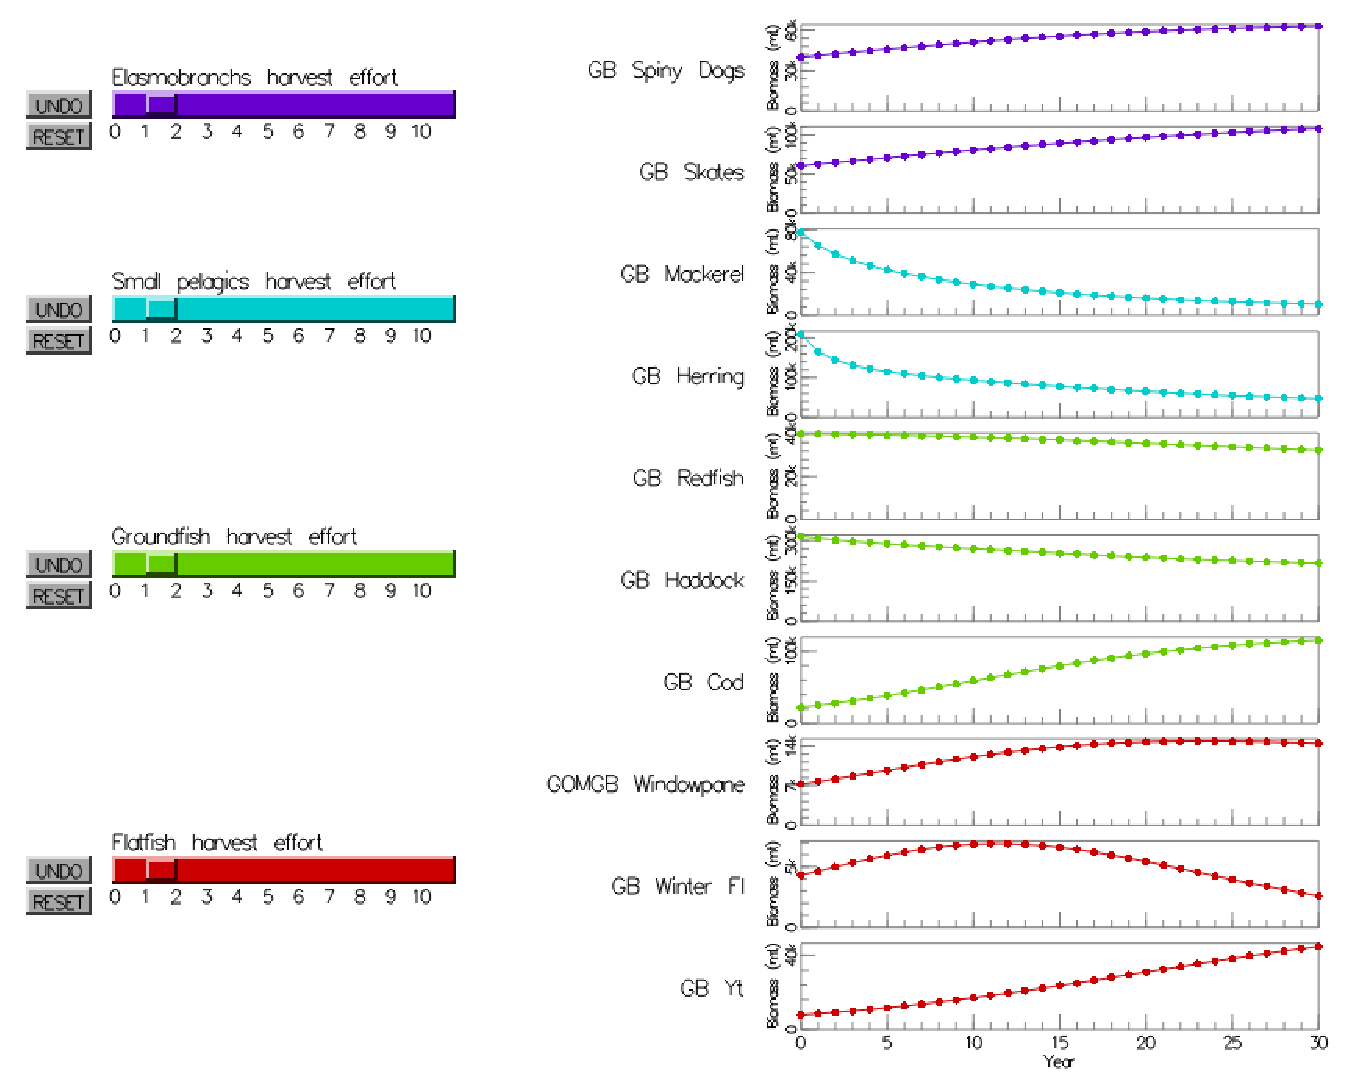
\includegraphics[width=12cm]{figures/eps/msprod_species.eps}
	\caption{The ``small multiples'' view of our MS-PROD visualization.}
	\label{fig:msprod_species}
\end{figure}

The alternative to the ``four panel'' view is to view each species on its own plot, which we call the ``small multiple'' view.  The main purpose of this view was to support the addition of arc graph connections between species, as are discussed later in Section~\ref{sec:interSpeciesArc}. Shown in Figure~\ref{fig:msprod_species}, each plot is sorted and colored according to functional group membership, using Cleveland's recommendations for chart size \cite{cleveland1988}.  The harvest effort sliders are also colored by functional group and positioned near the plots of the corresponding group.  This allows for the ability to differentiate between direct and indirect effects of changes in harvest effort.

With each species on its own plot, it is much easier to interpret the biomass predictions of an individual species, since the $y$-dimension of a plot needs to be scaled to the data of one species only.  It is also seasier to perceive increases or decreases in biomass because no species suffer from the ``flattening'' that can occur when a series is displayed on the same plot as a series that has significantly higher values.  On the other hand, this makes biomass comparison between species somewhat difficult because the user must either refer to the $y$-axis labels or hover over a specific point on a chart, which causes a label to appear, in order to determine the absolute value of the biomass at a point in time.

\subsubsection{Absolute Biomass Indicators}

\begin{figure}[h]
	\centering
	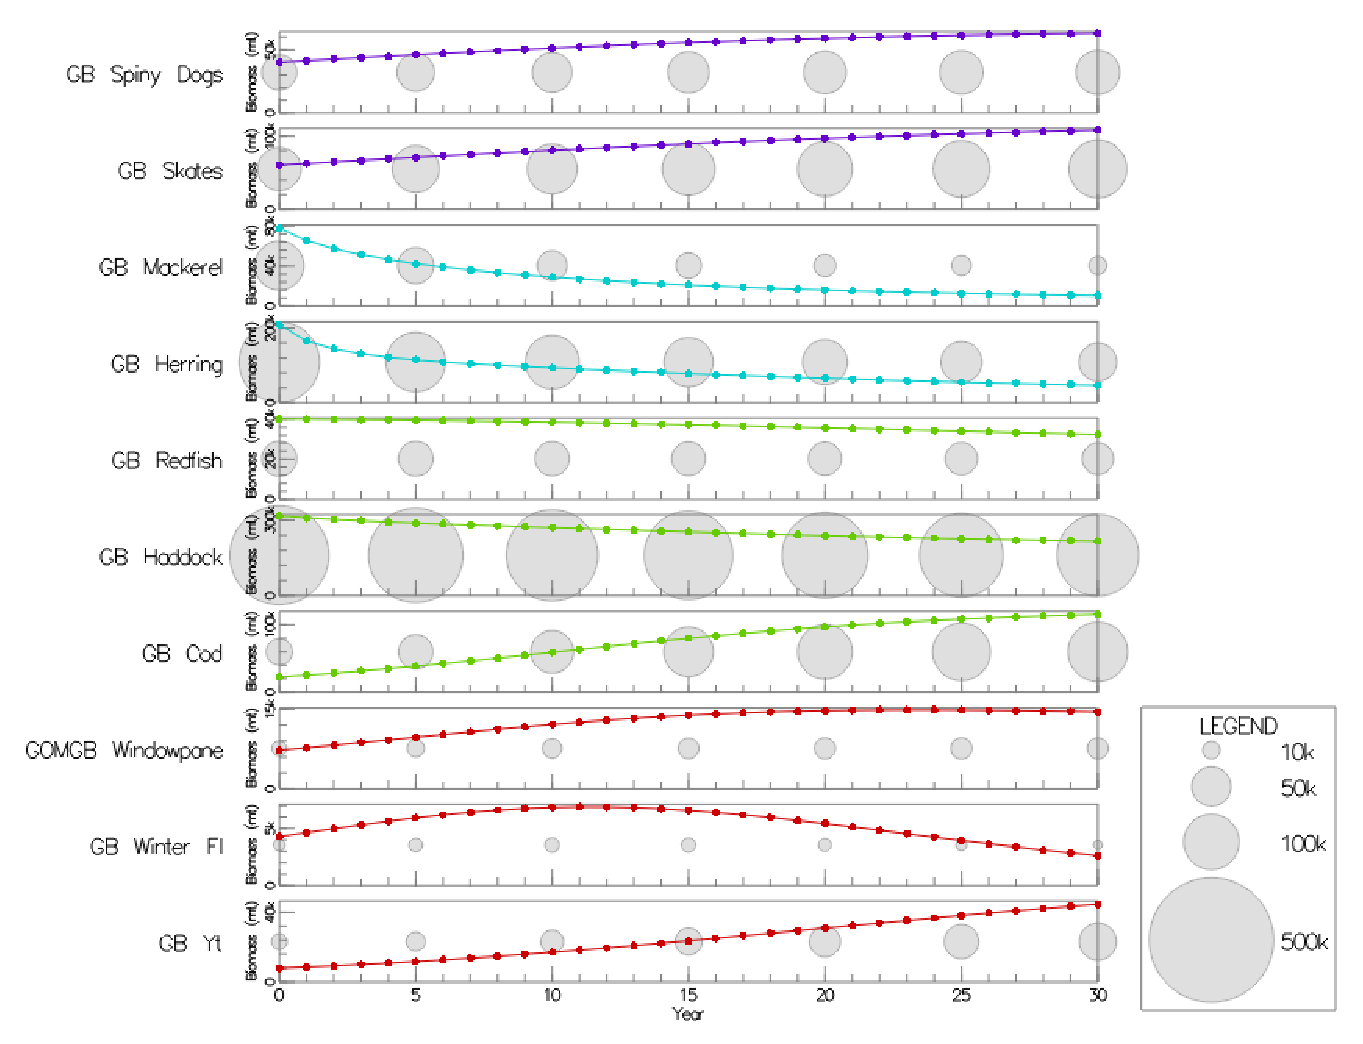
\includegraphics[width=11cm]{figures/eps/msprod_abssize.eps}
	\caption{Absolute biomass indicators overlaying the ``small multiples'' view.}
	\label{fig:msprod_abssize}
\end{figure}

Absolute biomass indicators, seen in Figure~\ref{fig:msprod_abssize}, were introduced to show how biomass changes over time by showing the absolute biomass of the population as the area of a circle.  This makes comparison across species possible.  To avoid occlusion, these indicators are drawn every five years within the thirty-year time span.

\section{Visualization of Change}

\begin{figure}
\centering
	\begin{subfigure}[b]{0.8\textwidth}
		\centering
		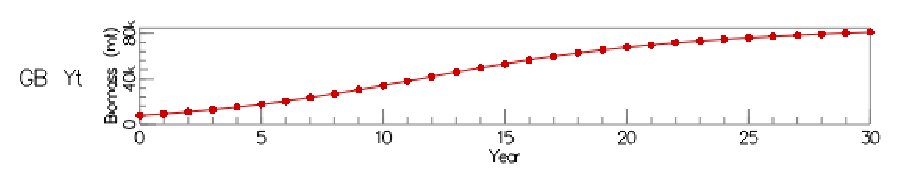
\includegraphics[width=11cm]{figures/eps/msprod_change_none.eps}
		\caption{Change shown by interaction.}	
		\label{fig:changeNone}
	\end{subfigure}	\\
	\begin{subfigure}[b]{0.8\textwidth}
		\centering
		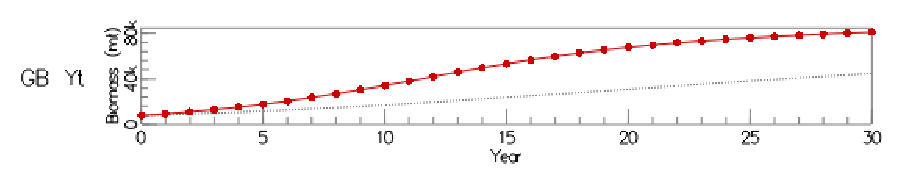
\includegraphics[width=11cm]{figures/eps/msprod_change_line.eps}
		\caption{The status quo is shown as the dotted gray line.}
		\label{fig:changeLine}
	\end{subfigure} \\
	\begin{subfigure}[b]{0.8\textwidth}
		\centering
		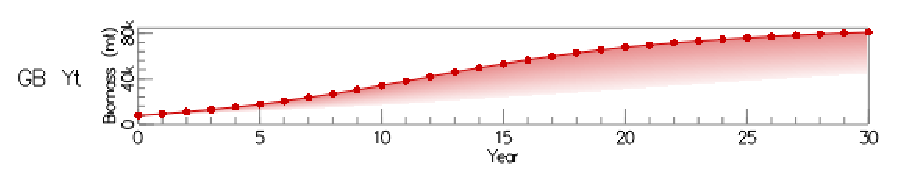
\includegraphics[width=11cm]{figures/eps/msprod_change_blend.eps}
		\caption{The area between the status quo graph and the new forecast is shaded.}
		\label{fig:changeBlend}
	\end{subfigure}
	\caption{The three options for depicting change between current biomass predictions and baseline predictions.}
	\label{fig:changeTypes}
\end{figure}

In order for modelers and other stakeholders to understand and compare decisions, the ability to perceive changes in biomass resulting from changes in the fishing effort is required.  Therefore, we have introduced a feature that allows the user to compare the forecast effects of a change in fishing effort compared to the forecasts of the \textit{status quo} [baseline]. There are three alternatives for displaying forecast differences with the baseline.  The first is to simply have the biomass plots change instantaneously as the harvest effort sliders are adjusted, as in Figure~\ref{fig:changeNone}.  The second is a dotted gray line which shows the forecast of the baseline in addition to the current forecast, shown in Figure~\ref{fig:changeLine}.  The third is a shaded area originating from the curve of the current forecast that diminishes in opacity as it approaches the curve of the baseline forecast, as in Figure~\ref{fig:changeBlend}.

\begin{figure}[h]
	\centering
	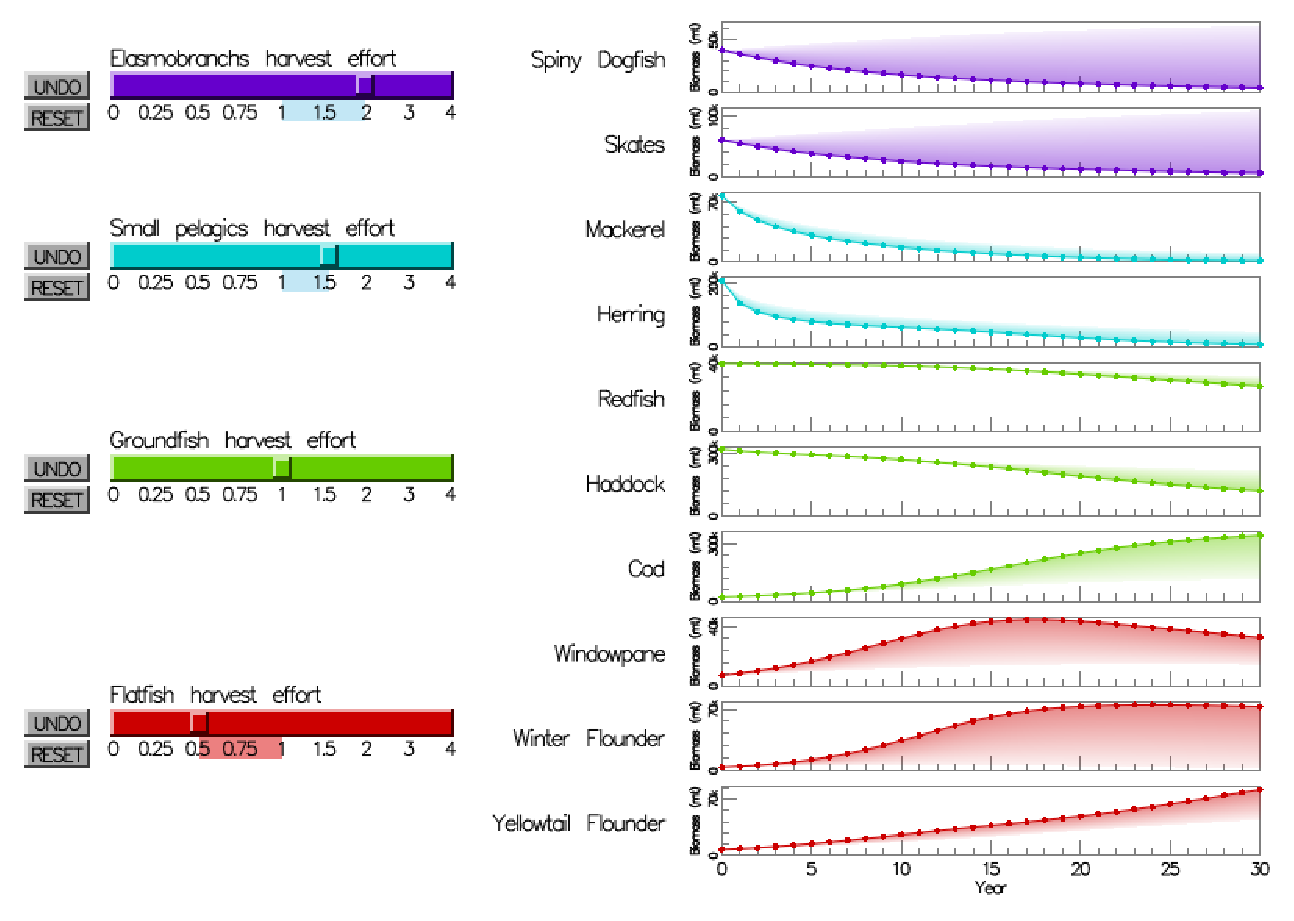
\includegraphics[width=12cm]{figures/eps/msprod_change.eps}
	\caption{Showing change between different effort values.}
	\label{fig:msprod_change}
\end{figure}

Figure~\ref{fig:msprod_change} shows all of the time series in the ``small multiples'' view with the effort sliders and the blended change option enabled.  Again, the blended area in a line chart is colored from the current biomass line to the line as it was when the baseline was set; a colored area above the line indicates the biomass declined, while a colored area beneath represents the biomass increased---e.g., the ``skate'' population declined dramatically with the new effort values, the ``winter flounder'' population increased due to the changes, and ``redfish'' seemed to be unaffected.

Underneath each slider, a colored rectangle---if present---indicates differences from the baseline effort settings.  Blue indicates the effort value has been increased since the baseline was set---e.g., again in Figure~\ref{fig:msprod_change}, the effort for ``elasmobranchs'' was originally set to 1.0 and now it is approximately 2.0.  Red represents the effort value has been decreased since the baseline was set---e.g., the effort for ``flatfish'' was originally set to 1.0 and now it is approximately 0.5.

This feature is available in both the ``four panel'' and ``small multiples'' views.  The baseline effort setting can be defined at any time with a simple button at the top of the screen.  This resets the baseline as the current slider settings.  Buttons are also available to undo or reset changes to the effort values.

\section{Visualization of Causal Relationships}
%\label{sec:arc}

Understanding of the model requires understanding of the underlying relationships between species---namely, \textit{predation} and \textit{competition}---and \textit{harvest}.  As defined earlier, predation is when one species consumes another and competition accounts for any way species might impact another in a way that is not predation.  Harvest is process of humans trying to catch fish in the wild.  Our interface must explain to users which species impact each other, how harvesting impacts the species, and the magnitude of those relationships.  We have chosen to illustrate these relationships with a node-link diagram, where the nodes are the time series of the fish species and the harvest effort sliders.

\subsection{Inter-Species Relationships}
\label{sec:interSpeciesArc}

\begin{figure}
\centering
	\begin{subfigure}[b]{0.33\textwidth}
		\centering
		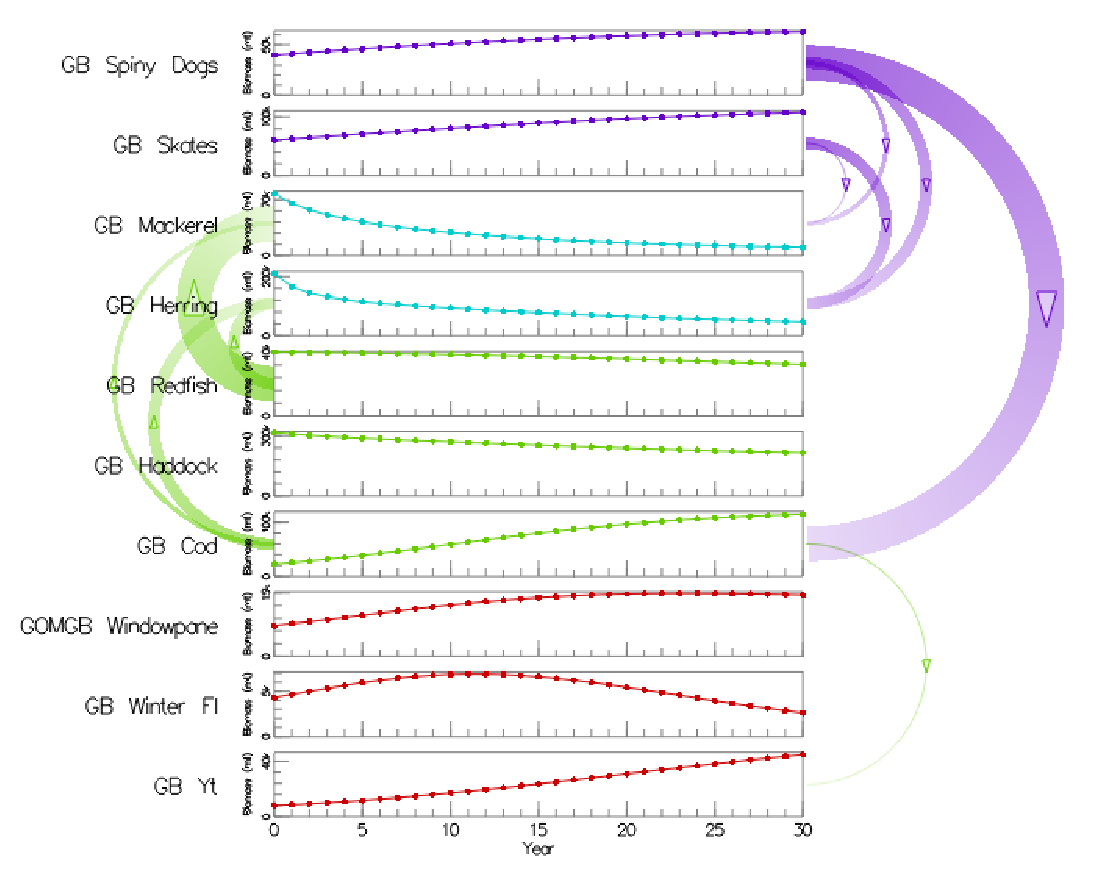
\includegraphics[width=1\textwidth]{figures/eps/arcs_predation.eps}
		\caption{Predation arcs.}
		\label{fig:arcsPredation}
	\end{subfigure}	
	\begin{subfigure}[b]{0.33\textwidth}
		\centering
		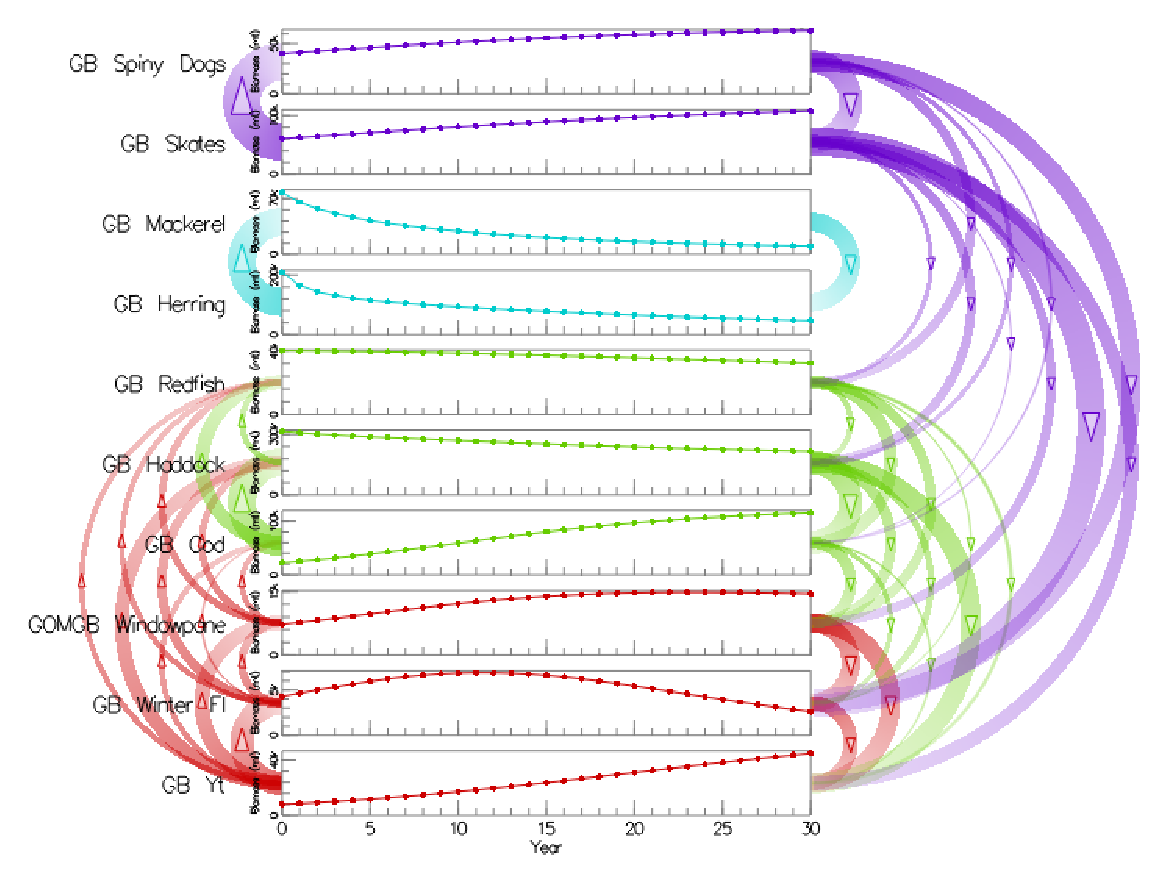
\includegraphics[width=1\textwidth]{figures/eps/arcs_interaction.eps}
		\caption{Competition arcs.}
		\label{fig:arcsCompetition}
	\end{subfigure}
	\begin{subfigure}[b]{0.32\textwidth}
		\centering
		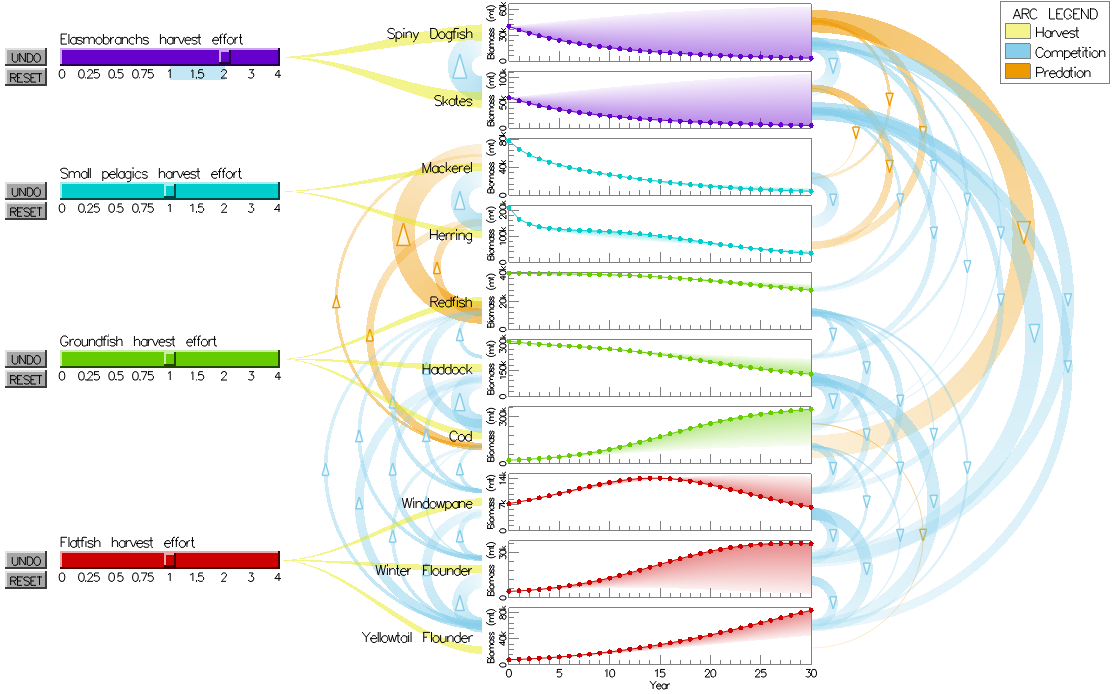
\includegraphics[width=1\textwidth]{figures/eps/arcs_static.eps}
		\caption{Both types of arcs.}
		\label{fig:arcsBoth}
	\end{subfigure}
	\caption{Static arcs drawn between species charts to represent relationships.}
	\label{fig:betweenSpeciesArcs}
\end{figure}

The inter-species relationships are illustrated with arc diagram network visualizations between time series, as in Figure~\ref{fig:betweenSpeciesArcs}.  In the input parameter file, predation and competition coefficient matrices are defined to represent the relationship between each pair of species.  Each non-zero coefficient is represented with an arc connecting the time series plots of the corresponding species.  This is only available in the small multiples view because multiple species are represented in each line chart of the four panel view.

The arc diagram was selected over other network visualizations because it is easily combined with the small multiples.  A separate node-link diagram, such as one with a force-directed layout, may have been confusing because it would require the user to mentally associate nodes in the network with line charts.  An arc diagram does not suffer from this problem since, in our case, the time series themselves are the nodes.  Furthermore, the arc diagram enhances the entire visualization without occluding the time series.  Arc diagrams are also well suited to smaller datasets with clusters of nodes, which applies to our dataset since the fish are segmented into functional groups.

\subsubsection{Directionality}

\begin{figure}[h]
	\centering
	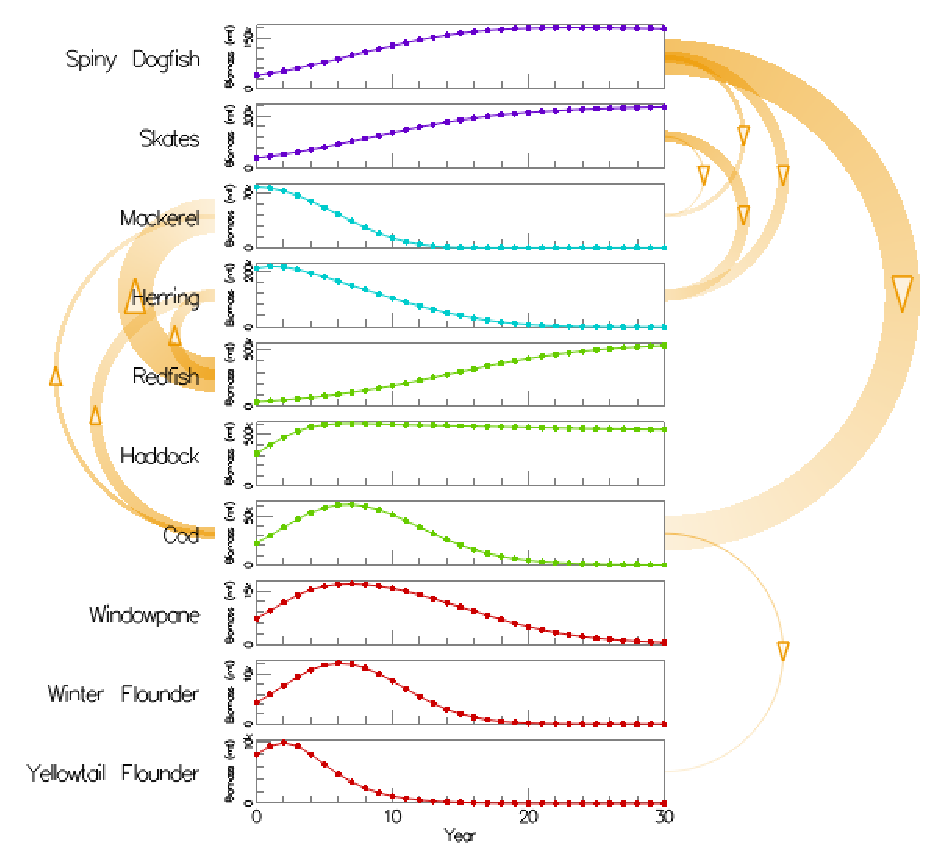
\includegraphics[width=0.85\textwidth]{figures/eps/arcs_directionality.eps}
	\caption{Static predation arcs with directionality indicated by a triangular arrow, fading color intensity, and clockwise direction.}
	\label{fig:arcs_directionality}
\end{figure}

These relationships, predation and competition, both imply directionality, where one species of fish is the ``source'' and the other species is the ``recipient.''  Therefore, our arcs have been drawn with fading opacity to indicate the direction, since Holten and van Wijk recommended a dark-to-light representation for an intensity-based cue \cite{holten2009}.  Additionally, our arcs follow a clockwise direction.  This is necessary because there may be reciprocal ``Fish A affects Fish B'' and ``Fish B affects Fish A'' relationships, especially for the competition type of relationship, so arcs must be drawn on both sides of the time series, as seen in Figure~\ref{fig:betweenSpeciesArcs}.  Additionally, triangular marks have been drawn in the middle of the arcs to point from the source species to the recipient species.  These three directionality cues can be seen in Figure~\ref{fig:arcs_directionality}.

\subsubsection{Arc Type}

The interface provides a few options for viewing the inter-species relationships.  Firstly, users have the ability to view either predation as in Figure~\ref{fig:arcsPredation}, competition as in Figure~\ref{fig:arcsCompetition}, or both as in Figure~\ref{fig:arcsBoth}.  Secondly, the arcs can be viewed statically, dynamically without animation, or dynamically with animation; these three arc types are described below.  Regardless of the selected arc type, all predation arcs are colored orange and all competition arcs are colored sky-blue.  The user can mouse over a particular arc, which causes that arc to highlight---while the other arcs fade---and displays a label which spells out the relationship in words and shows the input parameter matrix original coefficient---e.g., ``Skates compete with Winter Flounder (0.6).''

\paragraph{Static}

With the static style of the arcs, all arcs are drawn at all times, as shown in all three subfigures of Figure~\ref{fig:betweenSpeciesArcs}.  The width of an arc corresponds to the magnitude of the relationship, as defined in the predation coefficient matrix or the competition coefficient matrix in the original parameter file.   A benefit of this type of arc is that it is possible to see all interactions between the species at all times.  However, the downside is that viewing all arcs at once can be overwhelming because the display becomes somewhat cluttered.

\paragraph{Dynamic}

Dynamic arcs, shown in Figure~\ref{fig:arcs_dynamic}, were motivated by need to eliminate or at least reduce the visual clutter created by the static arcs.  We also considered the fact that many users might use our interface as a means of comparing two biomass forecasts that resulted from changes in fishing effort values.  Such users might wonder what specifically caused the differences between the two forecasts, especially if there are indirect, unintuitive effects.  Therefore, we designed dynamic arcs, which are drawn only selectively to help explain the differences in between the current forecast and the baseline forecast.

In dynamic mode, the width of each arc is proportional to a weight $w$:

\begin{align}
w = \frac{100000}{r_{0} + 100000} \cdot (s_{30} - s_{30}')
\end{align}
where $r_{0}$ represents the initial biomass of the recipient species, $s_{30}$ is the biomass at year 30 for the source species according to the current forecast, and $s_{30}'$ is the biomass at year 30 for the source species according to the baseline forecast.  If the source species biomass at year 30 did not change between the species, then $(s_{30} - s_{30}')$ equals zero, resulting in a $w$ of zero, so the arc will not be drawn.  In other words, the source species must have experienced change between the two forecasts in order to possibly explain a change that occurred in the recipient species; if there was no such change, then no arc is drawn.  The width of the arc increases as the difference between the two forecasts for the source at year 30 increases.  The portion of the equation with $r_{0}$ is to prevent arcs from being drawn simply because the source species experienced an increase or a decrease.  If the recipient biomass at time zero is sufficiently large, then the impact the source species will have on the recipient is not as significant as it would have been if the initial recipient biomass was small.

To summarize, the width of an arc in dynamic mode is (a) proportional to the difference for the final values of the baseline and current forecasts for the source species and (b) inversely proportional to the initial biomass of the recipient species.  Therefore, no arcs are drawn when the current forecast and the baseline forecast are the same.  As the sliders are adjusted either positively or negatively, more arcs may appear to assist in explaining indirect effects.  An arc grows in width as the source species experiences more dramatic change between the forecasts.

Additionally, the weight $w$ is negative if $s_{30} < s_{30}'$.  This is significant in explaining \textit{how} the change in the source species affects the recipient species---i.e., was the change that the source species experienced ``good'' or ``bad'' from the perspective of the recipient species?  Both relationships, competition and predation, inhibit the growth of the recipient species because the source species either consumes the recipient species itself or its resources.  Therefore, if the source species biomass decreases, then the recipient species biomass may be able to grow more.  Of course, other species may be dampening the growth of the recipient species, so the recipient species may not necessarily experience a growth, but the potential exists.  Conversely, if the source species biomass increases, then the recipient species may suffer more and experience a decrease in biomass.  Therefore, it was necessary to indicate the signage of a dynamic arc.  We chose to use plus signs ($+$) for the cases where $w$ is negative---i.e., when the source species declines between forecasts which is ``good'' for the recipient species---and minus sign ($-$) for the cases where $w$ is positive---i.e., when the source species increases between forecasts which is ``bad'' for the recipient species---as Kadaba et al.\ used in their static causal visualizations \cite{kadaba2007}.  Plus signs were drawn in black and minus signs were drawn in white with a black outline to allow for some redundant coding.  Several sign glyphs are drawn along each arc to allow the user to easily determine the signage of a dynamic arc.

\begin{figure}[h]
	\centering
	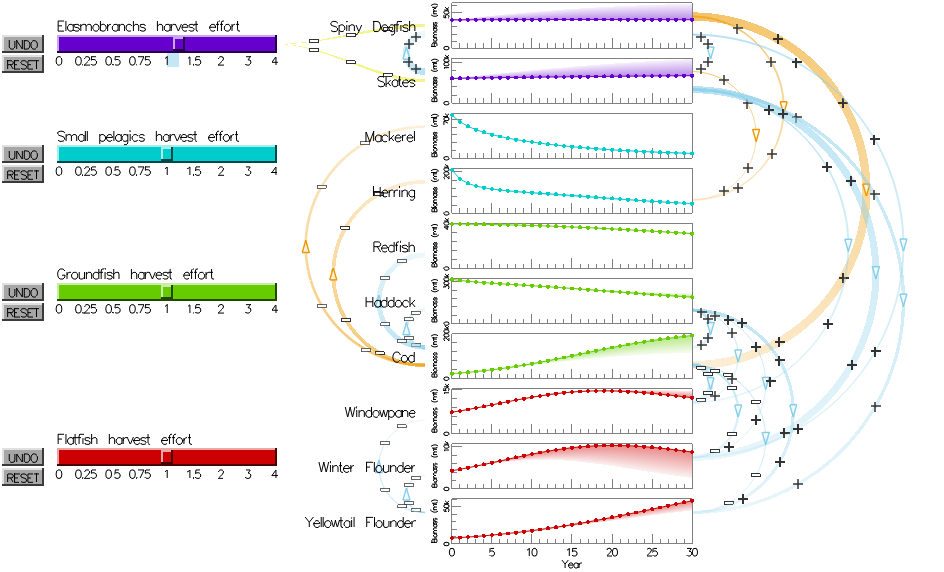
\includegraphics[width=0.98\textwidth]{figures/eps/arcs_dynamic.eps}
	\caption{Dynamic arcs drawn as a result of slightly increasing the fishing effort on elasmobranchs.}
	\label{fig:arcs_dynamic}
\end{figure}

Again, Figure~\ref{fig:arcs_dynamic} shows dynamic arcs which resulted from slightly increasing the fishing effort on elasmobranchs from 1.0 to about 1.25.  The spiny dogfish and skate biomasses both decreased as a result of the increase in fishing, as is indicated by the shaded area between the baseline forecast and the current forecast.  This is good from the perspective of all of the fish that either spiny dogfish or elasmobranchs predate on or compete with, therefore all of the arcs drawn from these two species show plus sign glyphs.  For example, spiny dogfish predate on cod, so the arc between them has plus signs.  The cod biomass increased, which seems to corroborate with the plus signs drawn on the arc.  There are also indirect effects that the arcs help to explain.  Cod competes with windowpane, so minus signs are drawn on the arc from cod to windowpane, which helps to explain the slight decrease in the windowpane biomass.

We have realized it is possible for dynamic arcs to be misinterpreted.  Users may incorrectly assume that absence of an arc indicates that the relationship is no longer present---e.g., if the predation arc from spiny dogfish to cod is not present, then the spiny dogfish are not eating the cod.  However, we believe that users will understand the true meaning of the arcs after a brief explanation---e.g., the arc between spiny dogfish and cod is no longer being drawn because there are no changes in the cod population that might be explained by the spiny dogfish.  When informally showing the model to users during and after development, we found that users properly interpreted the arcs after a demonstration or interaction with the model.  Another possible criticism of the dynamic arcs is that sometimes many arcs are drawn and it can become cluttered, such as when several sliders are pulled to the extremes.  However, generally less arcs are drawn in dynamic mode than static mode even in extreme cases.  Also, fishery managers may potentially be more interested in comparing the long-term effects of slight adjustments to fishing quota than dramatic adjustments that either eliminate fishing completely or wipe out entire stocks through overfishing.

\paragraph{Dynamic with Animation}

\begin{figure}[h]
	\centering
	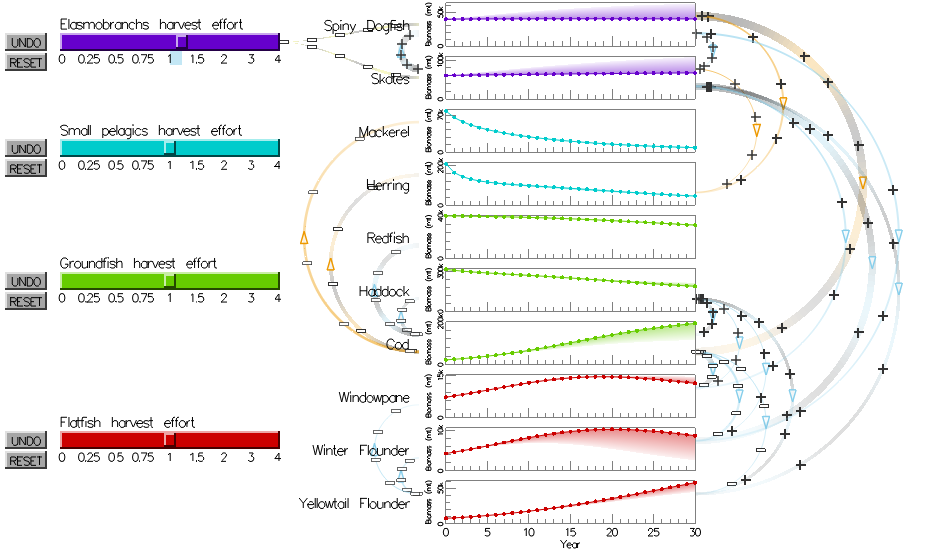
\includegraphics[width=0.98\textwidth]{figures/eps/arcs_dynamic_animated.eps}
	\caption{The same scenario as in Figure~\ref{fig:arcs_dynamic}, though with animated dynamic arc.}
	\label{fig:arcs_dynamic_animated}
\end{figure}

The third and final type for viewing the inter-species arcs is dynamic arcs with animation, seen in Figure~\ref{fig:arcs_dynamic_animated}.  In this mode, the rules for the appearance of arcs and their width is the same as in the non-animated dynamic version.  However, the plus ($+$) or minus ($-$) sign glyphs travel along the arc from the source species to the recipient species.  Additionally, the color of the arc alternates between gray and either blue for competition or orange for predation.  The alteration in color also moves from source to recipient.  Both of these cues help to highlight the directionality of the arc.

\subsection{Harvest Influences}

The other type of relationship that must be elucidated by our visualization is the harvest relationship.  While it is clear what the harvest effort value is for a particular slider, it could perhaps be clearer which species were directly affected by the harvest and how.  Therefore, we decided to draw a link is between a harvest type and a fish species, which corresponds to a fishing effort slider and a biomass small multiple, respectively, in our interface.  These links are drawn using Hermite spline curves which are colored yellow.  Harvest spline curves are drawn in the small multiples view whenever any type of arc is drawn.  There are three styles for determining the width of these spline curves, which correspond to the styles for inter-species arcs: static, dynamic, and dynamic with animation.  The controls for setting the inter-species arc style also set the harvest spline curve style.  

\subsubsection{Static}

\begin{figure}[h]
	\centering
	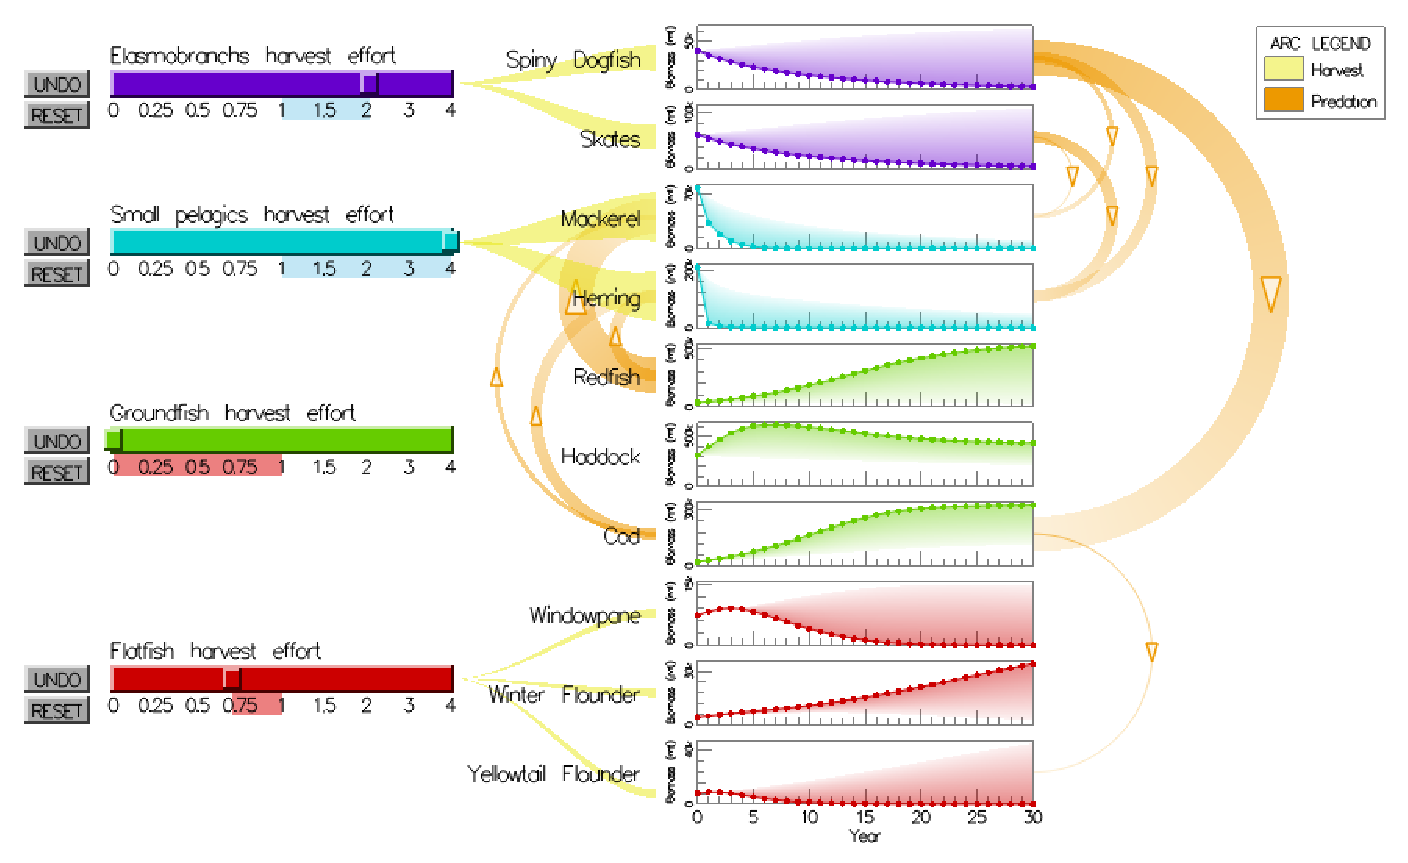
\includegraphics[width=0.98\textwidth]{figures/eps/harvest_splines.eps}
	\caption{Static harvest spline curves in yellow between effort sliders and the small multiples.}
	\label{fig:harvest_splines}
\end{figure}

In static mode, the harvest spline curve's width is directly proportional to the current value of the harvest slider, as in Figure~\ref{fig:harvest_splines}.  Therefore, when harvest effort for a specific functional group is set to zero (as it is for ``Groundfish''), then no harvest spline curves are drawn emerging from that harvest effort slider.  Likewise, the spline curves are their thickest when the matching effort slider is set to the maximum value of four (as it is for ``Small pelagics'').

\subsubsection{Dynamic}

Dynamic harvest splines can be seen in Figure~\ref{fig:arcs_dynamic}.  The width of a harvest spline in dynamic mode is proportional to the difference between the current value of the effort slider and the baseline value of the effort slider.  In other words, the width depends on a weight $w$:

\begin{align}
w = E - E'
\end{align}
where $E$ is the current effort and $E'$ is the baseline effort value for the functional group.  This is to help highlight and explain the differences between the baseline and current forecasts.   Therefore, when the harvest effort for a functional group has not been changed from the baseline, $w$ is zero and no harvest splines are drawn from that functional group's slider.

When $E' > E$ (i.e., when the harvest effort slider has been decreased), $w$ is negative.  Therefore, as with dynamic arcs for the inter-species relationships, the harvest splines have signage, which we interpreted from the perspective of the recipient---i.e., the fish being harvested.  Thus, when $w$ is negative, black plus sign ($+$) glyphs are drawn along the spline.  Conversely, when $w$ is positive, white minus sign ($-$) glyphs are drawn along the spline.  From the perspective of the fish, it is ``bad'' to be fished more and ``good'' to be fished less.  The meaning and design of these sign glyphs are the same as for the inter-species arcs.

\subsubsection{Dynamic with Animated}

Dynamic harvest spline curves, as in Figure~\ref{fig:arcs_dynamic_animated}, are drawn following the rules for non-animated spline curves, though with animation added.  The animation is similar to the animation for inter-species arcs:  the sign glyphs travel from the harvest effort slider to the species biomass small multiple chart and the color is alternated with gray to create a pulsing effect.  The intent was to give a clearer indication of the direction of the causal relationship.

\section{Visualization of Uncertainty}

\begin{figure}
\centering
	\begin{subfigure}[b]{0.45\textwidth}
		\centering
		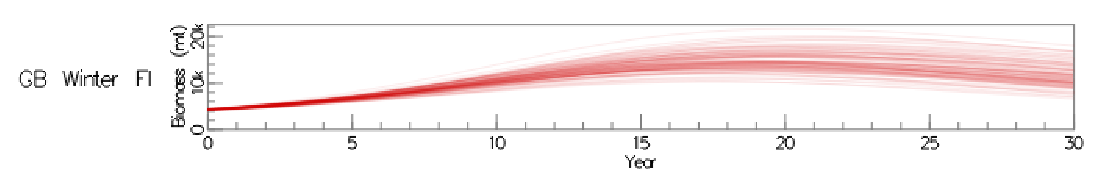
\includegraphics[width=6.5cm]{figures/eps/msprod_uncertainty_multline.eps}
		\caption{Multi-line.}
		\label{fig:uncertaintyStreak}
	\end{subfigure}	
	\begin{subfigure}[b]{0.45\textwidth}
		\centering
		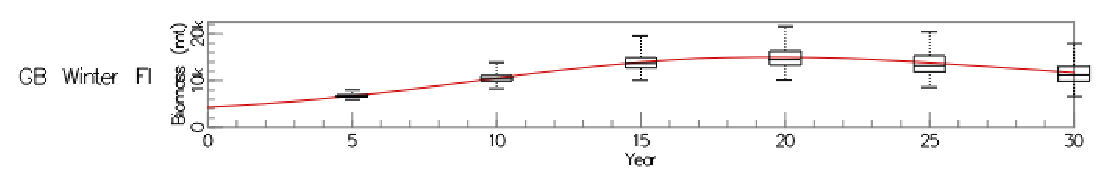
\includegraphics[width=6.5cm]{figures/eps/msprod_uncertainty_boxplots.eps}
		\caption{Box plots.}
		\label{fig:uncertaintyBoxplots}
	\end{subfigure} \\
	\begin{subfigure}[b]{0.45\textwidth}
		\centering
		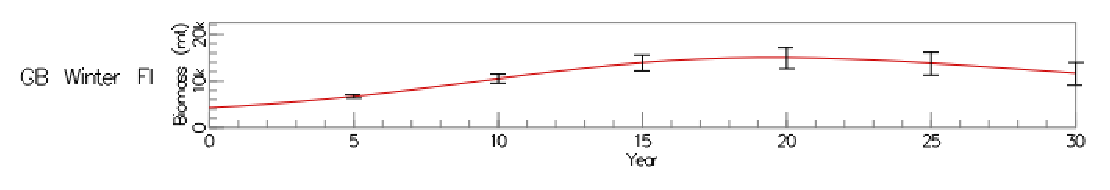
\includegraphics[width=6.5cm]{figures/eps/msprod_uncertainty_errorbar.eps}
		\caption{Error bars.}
		\label{fig:uncertaintyErrorbars}
	\end{subfigure}
	\begin{subfigure}[b]{0.45\textwidth}
		\centering
		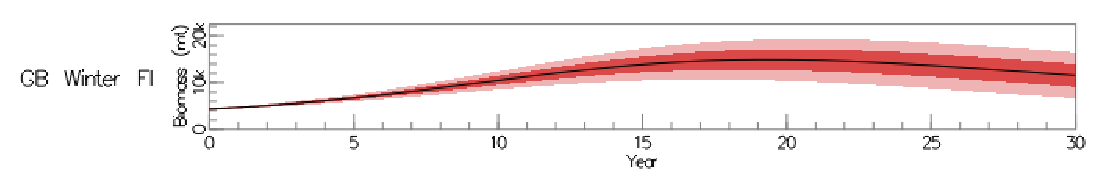
\includegraphics[width=6.5cm]{figures/eps/msprod_uncertainty_errorbands.eps}
		\caption{Error bands.}
		\label{fig:uncertaintyErrorbands}
	\end{subfigure}
	\caption{The four methods for visualizing uncertainty of MS-PROD model simulations.}
	\label{fig:uncertainty}
\end{figure}

Since models are simplifications of reality, their output is best understood as a range of expected values.  It is possible that a representation of uncertainty may aid decision making.  To add uncertainty visualization to the MS-PROD model, our interface can perform Monte Carlo simulations by jittering the non-zero input parameter values $\pm 10\%$ using a normal distribution.

The resulting uncertainty can be displayed in four styles.  First, a multi-line option shows the uncertainty by drawing one semi-transparent line for each run of the Monte Carlo simulation, as in Figure~\ref{fig:uncertaintyStreak}. This was inspired by Cox et al.'s new method for displaying hurricane tracks \cite{cox2013}.  The second option displays a traditional box plot every five years, as in Figure~\ref{fig:uncertaintyBoxplots}.  Third, in Figure~\ref{fig:uncertaintyErrorbars}, a summary line is drawn, with bars every five years.  Lastly, Figure~\ref{fig:uncertaintyErrorbands} shows a summary line in solid black line with bands.

In all options but the multi-line option, the user has the ability to display different statistical data in the selected style.  Users can select between mean and median for the ``summary'' lines.  Box plots, error bars, and error bands can represent either quartiles with minimum and maximum data values or two standard deviations.  This allows the user to easily explore the distribution of data under different representation with a few clicks of the mouse.  The multi-line option may appeal to less scientific users, while the other more traditional representations of statistical data may appeal to advanced users, such as modelers or fishery managers, but all users have all options at their disposal.

%to indicate the boundaries of the first, second (median), and third quartiles with whiskers stretching to the minimum and maximum values
% mean of all simulations is displayed as a line

\chapter{Evaluation}

The intention behind this work has been to develop an interactive visualization that effectively portrays the MS-PROD model and its implications.  We conducted two types of evaluations to determine which design alternatives were best for conveying this information: a formal evaluation of the arcs with novice users and an informal evaluation with expert users.  These two evaluations and the resulting findings are described in detail below. 

\section{Formal Evaluation of Dynamic Arcs}

We were interested in how different visualization alternatives enhance a user's understanding of the complex relationships between the fish species and the effects of those relationships.  In other words, is there a benefit to using dynamic, animated arcs---the most complicated representation of the relationships---over another method or even displaying no arcs at all?  To investigate this question, we designed and conducted a user study to measure the performance of different arc depiction alternatives.  The experimental conditions were as follows:

\begin{enumerate}[(A)]
\item No arcs
\item Static arcs
\item Dynamic arcs without animation
\item Dynamic arcs with animation
\end{enumerate}

Our hypothesis was that the Condition A would be the least effective, as it requires the user to guess why indirect or unexpected changes in biomass occurred since no arcs are drawn.  We also hypothesized that Condition C and Condition D would be more effective than Condition B, because dynamic arcs filter to show the relevant information, while static arcs show all information at once which could be overwhelming.  Finally, we hypothesized that Condition D would be at least slightly more effective than Condition C, since there are more visual cues for directionality with the animated arcs versus the non-animated arcs.

\subsection{Method}

The study was conducted at a screened-off table in a student union building at the University of New Hampshire.  A paid undergraduate research assistant conducted the study and responses from the study were graded by two paid undergraduate research assistants.

The research assistant conducting the experiment explained the MS-PROD model and our visualization to the participants, and showed a training example before leaving the participant to the experiment.  Each participant conducted the experiment task for only one of the four conditions.  Explanations and training phases were tailored according to the experimental condition---i.e., arcs were explained only for conditions B, C, and D; the meaning of dynamic arcs were explained only for conditions C and D.  Feedback about the quality of the participant's answers was given only during the training phase.  A single experiment lasted approximately fifteen minutes.

\subsection{Apparatus}

We conducted the experiment using a standard Dell laptop with an extra Dell monitor.  The window with the model visualization was maximized on the extra screen, while the window with the experiment questions was maximized on the laptop screen.  Participants used the mouse to interact with the model visualization and recorded their answers using the laptop keyboard.

\subsection{Participants}

There were 80 participants who took part in the study, all of which were recruited by a poster affixed to the backside of the privacy screen.  They could have been undergraduate or graduate students; we only required that participants had to be at least 18 years of age.  Participants were voluntary and were compensated with a pack of pens or a notebook.  They were required to read and sign an IRB consent form before participating in the study, shown in Appendix~\ref{sec:irbConsent}.

\subsection{Task}

Initially, all fishing effort sliders were set to the value of one.  Participants were instructed to increase or decrease the fishing effort of a specific functional group---e.g., \textit{``Using the sliders, double the harvest effort on elasmobranchs.''}  An example of this type of instructional window as it appeared to participants is shown in Figure~\ref{fig:eval_inst}.

\begin{figure}[h]
	\centering
	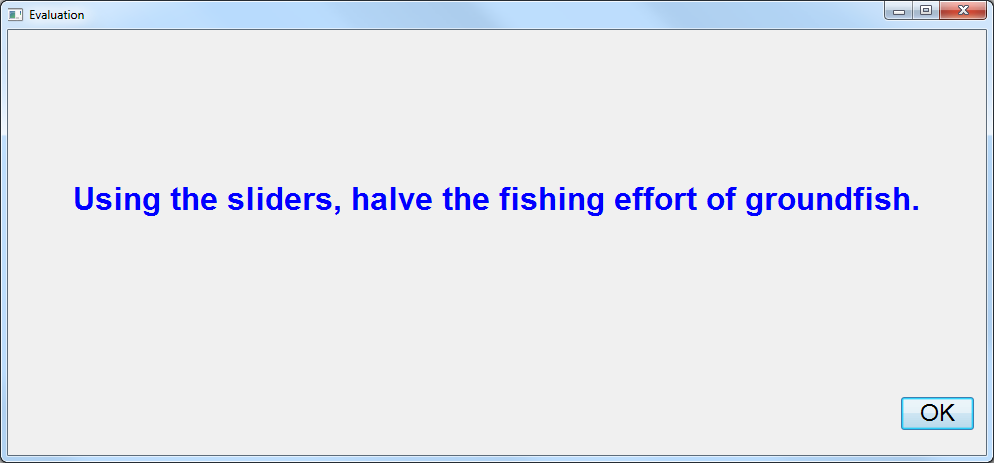
\includegraphics[width=0.5\textwidth]{figures/png/eval_instr.png}
	\caption{An instructional window in the evaluation which guides the participant.}
	\label{fig:eval_inst}
\end{figure}

Next, the participants were asked to answer one or more questions of the form, ``\textit{What was the effect on (fish species)?}''  E.g., \textit{``What was the effect on haddock?''}  All questions, as well as their answers, can be seen in Appendix~\ref{sec:questions}, grouped together by instruction.  %The questions were designed so that sometimes the fish species was a member of the function group for which the effort was just adjusted, while other times the fish species was not a member of that functional group.

Users answered this ``What\ldots?'' question with one of five options from a drop-down menu:
\begin{itemize}
\item \textit{Increased a lot}
\item \textit{Increased a little}
\item \textit{Stayed about the same}
\item \textit{Decreased a little}
\item \textit{Decreased a lot}
\end{itemize}
An example of the evaluation window as it appeared to users is shown in Figure~\ref{fig:eval_what}.

%\begin{figure}[h]
%	\centering
%	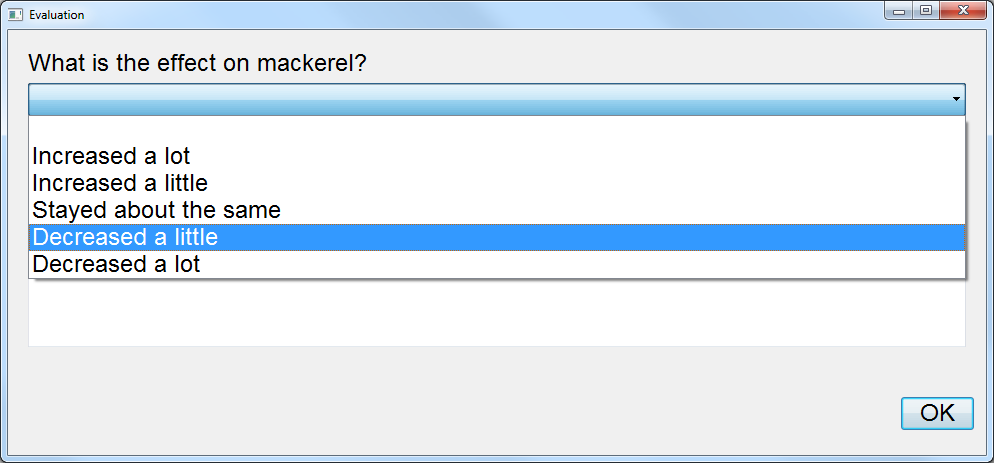
\includegraphics[width=0.48\textwidth]{figures/png/eval_what.png}
%	\caption{An example of evaluation window where users recorded their answers to the ``What\ldots?'' questions.}
%	\label{fig:eval_what}
%\end{figure}



\begin{figure}
\centering

\subfigure[The drop-down for selecting ``What\ldots?'' answers.]{\label{fig:eval_what}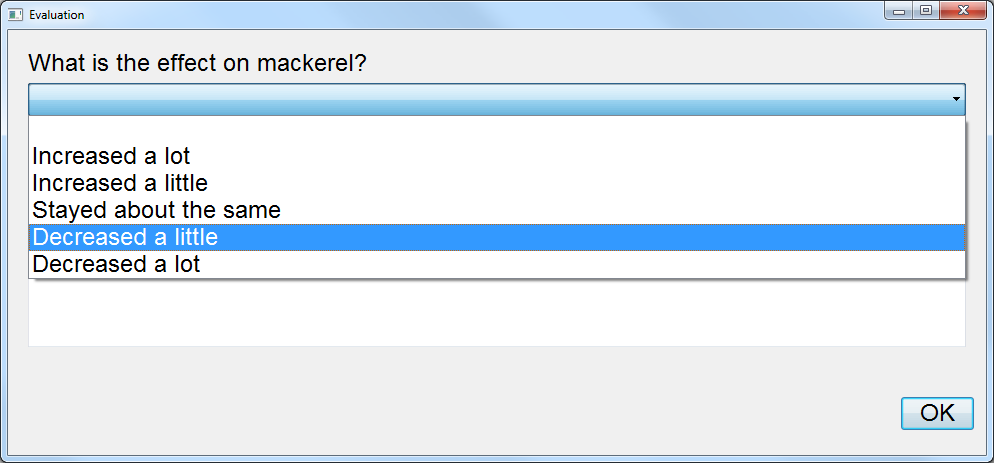
\includegraphics[width=0.48\textwidth]{figures/png/eval_what.png}} 
\subfigure[The text box for entering ``Why?'' answers.]{\label{fig:eval_why}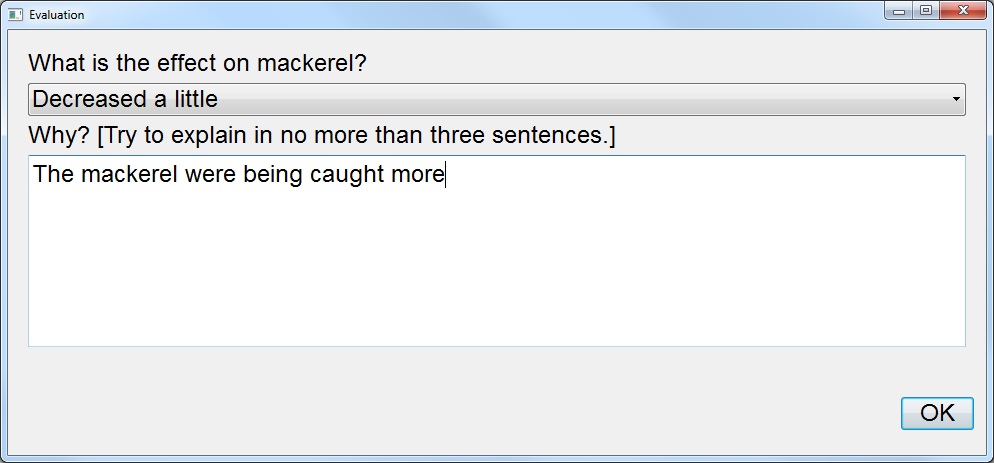
\includegraphics[width=0.48\textwidth]{figures/png/eval_why.png}}

	\caption{Examples of the windows where participants entered answers.}
	\label{fig:eval}
\end{figure}




Finally, the user was asked, ``\textit{Why? [Try to explain in no more than three sentences.]}''  A large text box was provided for the participant to type a response.  This is shown in Figure~\ref{fig:eval_why}. If this question was the last question in its set, then the sliders were all reset to one and a new instruction was given for the next set of questions until all questions were answered. 

%\begin{figure}[h]
%	\centering
%	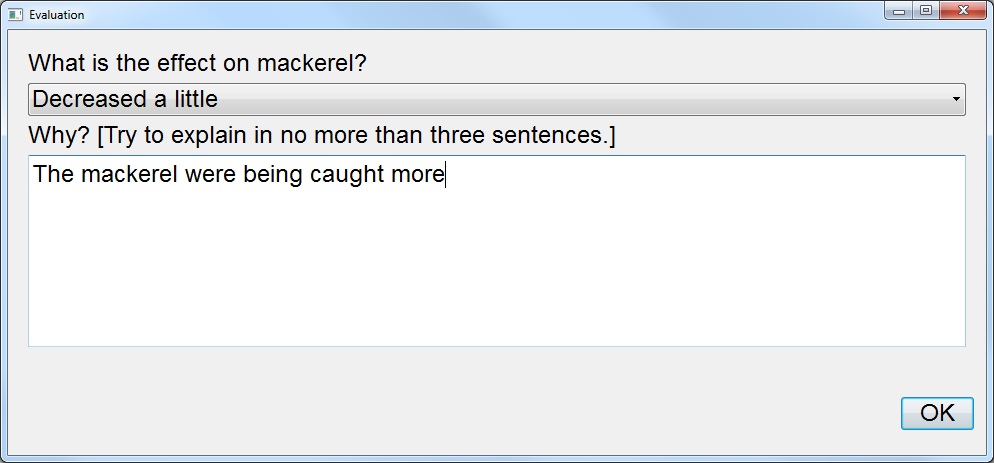
\includegraphics[width=0.48\textwidth]{figures/png/eval_why.png}
%	\caption{An example of evaluation window where users recorded their answers to the ``Why?'' questions.}
%	\label{fig:eval_why}
%\end{figure}

The questions were designed to fit in one of two difficulty categories:
\begin{itemize}
\item First-order
\item Higher-order
\end{itemize}

First-order questions asked about a fish species whose biomass changed directly as a result of increased or decreased harvest effort.  In other words, the fish was a member of the functional group whose harvest effort was changed and either (a) its biomass decreased due to increased harvest effort or (b) its biomass increased due to decreased harvest effort---e.g.,  increase harvest on A $\rightarrow$ biomass of A decreases.  There were three questions of this type.

Higher-order questions concerned a fish species whose biomass changed from a second-order or third-order effect.  In this case, the fish may or may not have been a member of the functional group for which the fishing effort changed.  If the fish was a member of the functional group, then perhaps its biomass did not change as expected because of the effects of competition or predation with other members of the functional group.  If the fish was not a member of the functional group for which fishing effort changed, then its biomass may have changed because of competition or predation with a member of that functional group---e.g., increase harvest on A $\rightarrow$ biomass of A decreases $\rightarrow$ biomass of B increases because A eats B.  More complex explanations involving several inter-species relationships are also possible---e.g., increase harvest on A $\rightarrow$ biomass of A decreases $\rightarrow$ biomass of B increases because A eats B $\rightarrow$ biomass of C decreases because B eats C.  There were four higher-order questions. 

In total, there were three instructions for adjusting the harvest effort and seven questions.  All participants were given the same instructions and asked the same questions in the same order, regardless of condition.

\subsection{Results}

\begin{figure}
\centering

\subfigure[``What\ldots?'' scores.]{\label{fig:resultsWhat}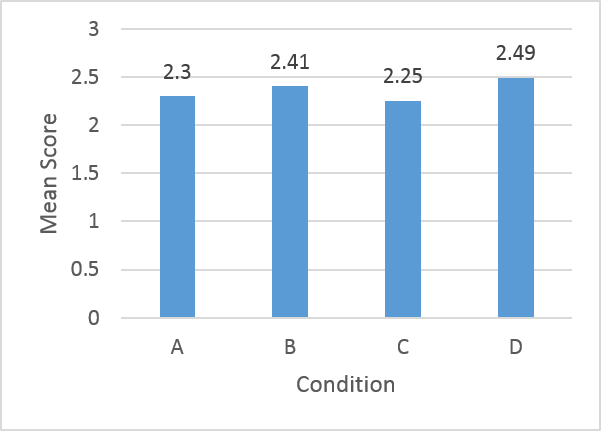
\includegraphics[width=0.32\textwidth]{figures/png/results_what.png}} 
\subfigure[First-order ``Why?'' scores.]{\label{fig:resultsWhy1}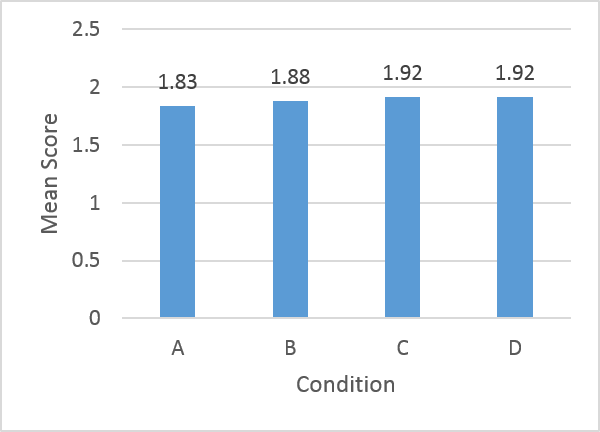
\includegraphics[width=0.32\textwidth]{figures/png/results_why1.png}}
\subfigure[Higher-order ``Why?'' scores.]{\label{fig:resultsWhy23}\includegraphics[width=0.32\textwidth]{figures/png/results_why23.png}}  

	\caption[Results of the formal evaluation, shown as mean scores graphed by condition.]{Results of the formal evaluation, shown as mean scores graphed by condition.  Scores were assigned on a scale from 0 to 3.}
	\label{fig:results}
\end{figure}

The answers to the questions of the evaluation were graded on a scale of 0 (i.e., completely wrong) to 3 (i.e., completely correct), with partial points allowed.  ``What\ldots?'' questions, which were answered using a drop-down, were graded automatically by a script, while ``Why?'' questions were graded by two undergraduate graders.  The average of the two scores was taken and these averages were used in our analyses.  The correlation coefficient (Pearson's $r$) between the scores assigned by each grader was 0.744.

The summarized results of our evaluation can be found in Figure~\ref{fig:results}, where mean scores are shown by condition.  For our analyses, we divided the questions into three categories:
\begin{enumerate}
\item ``What\ldots?'' questions
\item First-order ``Why?'' questions
\item Higher-order ``Why?'' questions
\end{enumerate}
Separate ANOVAs (analysis of variance) were run with Tukey HSD (Honestly Significant Differences) tests for each of these three types of questions.  There were no significant differences between the four conditions for the seven ``What\ldots?'' questions and the three first-order ``Why?'' questions.    However, there was a significant effect for the four conditions with the higher-order ``Why?'' questions, shown by $([F(1, 76] = 12.6; p < 0.001)$ and the HSD test, with no other significant differences (see Figure~\ref{fig:resultsWhy23}).

\begin{figure}[h]
	\centering
	\includegraphics[width=0.85\textwidth]{figures/png/results_arts_science.png}
	\caption{Mean scores for arts versus sciences students for the higher-order ``Why?'' questions.}
	\label{fig:results_arts_science}
\end{figure}

Additional ANOVAs were run to look for effects of gender and whether the student was a ``science'' or liberal arts student.  We created a pseudo-category called ``science'' for participants who reported being part of the College of Engineering and Physical Sciences, College of Health and Human Services, College of Life Sciences, School of Marine Science and Ocean Engineering, Peter T. Paul College of Business and Economics, and the Thompson School of Applied Science; this included everyone except for participants from the College of Liberal Arts.  The gender and ``science'' versus liberal arts factors showed no significant effect on the higher-order ``Why?'' questions according to our analyses.  However, despite this, the effect for ``science'' versus liberal arts approached significance; the effects of this are illustrated in Figure~\ref{fig:results_arts_science}.  %The mean for science students in Condition A was over three times the mean for liberal arts students, while the gap was smaller for the other conditions.  This could possibly suggest that science students have a small advantage because they are used to analyzing time series in their classes, which helped them with the worst depiction of the inter-species relationships.

\subsection{Discussion}

Our results strongly suggest that using either static or dynamic arcs is better than using no arcs at all for asking more difficult (i.e., higher-order) questions about the complex, underlying relationships between the species.  The type of causal relationship depiction did not matter as much when it came to simpler (i.e., ``What\ldots?'' and first-order ``Why?'') questions.  For the ``What\ldots?'' questions, this is not surprising, as these questions were concerned with reading a change in a time series chart, for which the inter-species relationships were totally irrelevant.  Similarly, the first-order ``Why?'' questions involved direct effects of the changes in fishing effort, so understanding of the inter-species relationships was unnecessary.  Only the higher-order questions involved the competition and/or predation relationships, leading to a significance to the presence or absence of arcs.

Though the difference in mean score between ``science'' and liberal arts students, shown in Figure~\ref{fig:results_arts_science}, was not significant, it is interesting.  In Condition A (no arcs), the mean for science students was over three times the mean for liberal arts students.  This could possibly suggest that ``science'' students have more experience with quantitative analysis and reasoning, therefore they were able to perform better in the absence of arcs.  The gap narrowed in the other conditions; under Condition B (static arcs), ``science'' students had scores over twice as high as the liberal arts students on average, while the means were similar in Conditions C (dynamic arcs) and D (animated and dynamic arcs).  Again, there was not enough significance, so no conclusions should be drawn, but this may imply that dynamic arcs enabled liberal arts students to produce higher quality answers.  Perhaps an evaluation with more participants would produce a significant result concerning the type of student.

We had expected to see a higher correlation coefficient for the scores assigned by the two undergraduate graders.  However, despite our efforts to provide a thorough and detailed grading key (see Appendix~\ref{sec:gradingScheme}), perhaps the task of assigning scores was difficult due to its subjective nature.  Both the quality and the length of the answers provided by participants varied greatly; it would not be impossible for one grader to consider an answer to be sufficient, while another grader finds it slightly lacking.  This was an issue we had foreseen, but it was unavoidable because there would have been no way to structure the ``Why?'' questions to be multiple choice without feeding the answer to the participants.  We were more concerned with measuring the ability of the users to construct an answer with no assistance other than the visualization itself.

\section{Informal Evaluations}

%Originally, we had intended to conduct semi-structured interviews with expert users such as the original author models and fishery managers where we would ask the users to rate each alternative depiction of the different features.  However, we determined that would be a long and perhaps tedious task for each participant given the number of different depictions.  Therefore,
We interviewed three expert users in an informal environment in order to determine their preferences of the alternative depiction of the different features.  The informal interviews consisted of explaining and demonstrating the visualization to the participants and asking them to describe which alternative depictions they prefer, if any, and why.  Overall, the expert users who participated in the informal evaluations liked the visualization in general, particularly the dynamic, animated arcs.  More detailed findings of these informal evaluations are below; the comments were reconstructed from notes made in the meetings.

\subsection{Michael Fogerty and Robert Gamble} %Dr Fogerty

Dr.\ Michael Fogerty and Robert Gamble---members of the NOAA's National Marine Fisheries Services (NMFS) in Woods Hole, MA---are the original authors of the MS-PROD model with Jason Link.  We presented a prototype of the visualization in August 2013 and a more finalized visualization in January 2014.  The two of them have been pleased with the visualization.

Before we developed our visualization, they were using Microsoft Excel spreadsheets to graph the CSV output of the model after each run.  They reacted positively to the abilities to (a) change fishing effort parameters and see an instantaneous result and (b) easily perceive differences between forecasts that resulted from changes in fishing effort.  Dr.\ Fogerty suggested that the user should be able to set the baseline forecast at any moment, which we implemented.  Mr.\ Gamble expressed interest in keeping all alternative depictions in the final visualization, as he liked the ability to toggle between the various options.  He said he could see himself using the small multiples view to understand the relationships between the species, while he might use the four-panel view to prepare figures for future publications.

The feature that Dr.\ Fogerty and Mr.\ Gamble have been most enthusiastic about is the dynamic, animated arcs.  This feature was first demonstrated at a NMFS meeting on January 24, 2014.  Other members in attendance were also excited about the dynamic, animated arcs.  Mr.\ Gamble expressed that even sometimes he can become confused about the counter-intuitive effects of the underlying relationships and must refer to the predation and competition matrices in the original parameter file to understand them; the dynamic arcs eliminate the need for this extra work by making the relevant relationships more obvious.  Members in attendance were very interested in the potential to adapt the visualization to other models.  Furthermore, they believed the visualization would allow them to make convincing arguments to fishery managers or other import decision makers to use the MS-PROD model or similar models.

Dr.\ Michael Fogerty and Robert Gamble have been further developing the MS-PROD model to include types of fishing (e.g., bottom trawl, midwater trawl, long lines, dredges) with different catchabilities for each pair of fish species and fishing type.  They have also introduced climate factors (e.g., average sea floor temperature).  They have expressed interest in incorporating these new factors into the visualization, as well as the ability to include more species and/or functional groups.  Furthermore, Dr.\ Fogerty is interested in developing a version of the visualization that is compatible with browsers for usage by the general public.  However, Gamble expressed reluctance to use the actual names of fish species because this could result in over-interpretation of the results and suggested that generic names like ``Elasmobranch 1'' and ``Elasmobranch 2'' be used.

In general, Dr.\ Fogerty and Mr.\ Gamble were satisfied with the quality of the visualization.  Mr.\ Gamble said that he was not sure how to express what he wanted in a visualization when our collaboration began, but he saw what he had originally envisioned when he saw the finalized visualization.  

\subsection{David Goethel}

On April 1, 2014, we conducted an informal interview with David Goethel.  David Goethel is a biologist and fisherman based out of Hampton, New Hampshire, who has advised several state and federal fishery management boards and served on the New England Fishery Management Council.  As a fisherman, he catches all ten of the species used in the MS-PROD model throughout the year, as well as others.  He has been an advocate for moving toward a more sustainable approach to fishery management and is interested in models which can help illustrate that change is necessary.  

Mr.\ Goethel found both the small multiple and four panel views useful.  He did not have a preference over either view and said that he might choose which one to use depending on his intended audience or what he was investigating in the model.  Similarly, he said he liked all options for uncertainty visualization and would choose based on his audience; he might use error bands when presenting to the general public, but use box plots for fishery managers.  He had previously believed that stock assessments should be presented more like hurricane tracks, with multiple forecasts to show multiple opinions, therefore he found the range of forecasts shown in the uncertainty view to be particularly helpful.

As for the different depictions of change, Mr.\ Goethel preferred the blended, shaded area between the two forecasts over instantaneous change only or the dotted line for the previous forecast.  He said he would always use the blended option because it was more informative.  For understanding the relationships between fish, he preferred the dynamic, animated arc over all other options.  This option allows the user to ``follow the flow [of the relationships] more easily,'' while he found it ``harder to see the conclusion'' of the effects of the harvest without animation.  He was excited to see a visualization of these relationships because they can be counter-intuitive even to someone with as much experience as him.

Overall, Mr.\ Goethel was interested in the model, saying that its visualization would help to convince people that more complex models like MS-PROD are necessary.  He said fishery managers typically prefer single species models and make decisions for ten-year periods.  However, Mr.\ Goethel finds it important to considering multiple species as well as other factors and to think about management for longer time periods, like MS-PROD.  He said that MS-PROD ``might reflect reality more,'' and our visualization might help to persuading managers of this.  He said he recommended restricting access of the model to scientific community only for now and waiting before presenting it to the general public to avoid unexperienced users from drawing incorrect conclusions.

\chapter{Conclusion}

A long-term goal of this thesis has been to help the fishery management community make informed decisions with the use the MS-PROD model through our interface.  Declaring whether we achieved this long-term goal depends on public unveiling of the MS-PROD model by its original authors and time to determine if it actually benefits managers, fishermen, and other significant stakeholders.  On the other hand, the short-term goal of this thesis has been develop an interactive visualization which would enhance understanding of a complicated, multi-species production model, MS-PROD.  More specifically, we investigated the effectiveness of different methods for depicting causal relationships.  To measure this objectively, we conducted an evaluation of the different depictions of the predation and competition relationships between the ten key species of the MS-PROD model.



\bibliographystyle{plainnat}

\bibliography{sources}

\begin{appendices}

\chapter{MS-PROD Input Parameters}

%Guild Membership	Flatfish	Groundfish	Groundfish	Flatfish	Flatfish	Groundfish	Small pelagics	Small pelagics	Elasmobranchs	Elasmobranchs
%$N_0$ & 8000 & 22563 & 316000 & 4301 & 7288 & 40048.8 & 209400 & 77600	60683 & 40000 \\
%$K$ & 230000 & 700000 & 700000 & 230000 & 230000 & 700000 & 350000 & 350000 & 450000 & 450000 \\						
%$r$ & 0.66 & 0.64 & 0.52 & 0.74 & 0.6 & 0.232 & 0.62 & 0.32 & 0.2 & 0.2 \\
Following are the input parameter values used for the development and evaluation of our visualization to the MS-PROD model.  These values were given to us by one of the model authors, Robert Gamble, and were unchanged except for catchability and effort.  In MS-PROD, effort ($E$) and catchability ($q$) can be set to different values for each of the thirty years for each species.  However, we kept these values the same across all years to simplify the controls needed to interact with the model.  Some terms have been abbreviated to allow these tables to fit; the abbreviations are defined following the tables.  Additionally, the names of the species did not fit into the coefficient matrices, therefore letters were assigned to each species in the first table for use in subsequent tables.


{\rowcolors{2}{gray!10}{gray!3}
\addvbuffer[2em 2em]{ \begin{tabular}{ | l | l | r | r | l | l | r | r | r | } \hline
\rowcolor{gray!35} \textbf{Species} & \textbf{Guild} & \textbf{$N_0$} & \textbf{$K$} & \textbf{$r$} & \textbf{$q$} & \textbf{$E$} & \textbf{Dem.} & \textbf{Pel.} \\ \hline
(a) Yellowtail Fl. & F & 8000 & 230000 & 0.66 & 0.1 & 1 & 1 & 0 \\ 
(b) Cod & G & 22563 & 700000 & 0.64 & 0.22 & 1 & 1 & 0 \\ 
(c) Haddock & G & 316000 & 700000 & 0.52 & 0.28 & 1 & 1 & 0 \\ 
(d) Winter Fl. & F & 4301 & 230000 & 0.74 & 0.3 & 1 & 1 & 0 \\
(e) Windowpane & F & 7288 & 230000 & 0.6 & 0.25 & 1 & 1 & 0 \\ 
(f) Redfish & G & 40048.8 & 700000 & 0.232 & 0.2 & 1 & 1 & 0 \\ 
(g) Herring & SP & 209400 & 350000 & 0.62 & 0.24 & 1 & 0 & 1 \\
(h) Mackerel & SP & 77600 & 350000 & 0.32 & 0.14 & 1 & 0 & 1 \\
(i) Skates & E & 60683 & 450000 & 0.2 & 0.13 & 1 & 1 & 0 \\
(j) Spiny Dogfish & E & 40000 & 450000 & 0.2 & 0.13 & 1 & 1 & 0 \\ \hline
\end{tabular}
}
}

\section{Competition Coefficient Matrix}

{\rowcolors{2}{gray!10}{gray!3}
\addvbuffer[1em 2em]{ \begin{tabular}{ | l | l | l | l | l | l | l | l | l | l | l | } \hline
\rowcolor{gray!35} & (a) & (b) & (c) & (d) & (e) & (f) & (g) & (h) & (i) & (j) \\ \hline
on (a) & 0 & 0.05 & 0.424 & 0.3 & 0.4 & 0.076 & 0 & 0 & 0.3 & 0 \\
on (b) & 0.12 & 0 & 0.5 & 0.05 & 0.12 & 0.276 & 0 & 0 & 0.01 & 0.05 \\
on (c) & 0.3 & 0.6 & 0 & 0.2 & 0.15 & 0.125 & 0 & 0 & 0.2 & 0.1 \\
on (d) & 0.5 & 0.101 & 0.141 & 0 & 0.4 & 0.041 & 0 & 0 & 0.6 & 0.4 \\
on (e) & 0.32 & 0.248 & 0.233 & 0.18 & 0 & 0.219 & 0 & 0 & 0.2 & 0 \\
on (f) & 0.119 & 0.3 & 0.132 & 0.12 & 0.15 & 0 & 0 & 0 & 0.1 & 0.2 \\
on (g) & 0 & 0 & 0 & 0 & 0 & 0 & 0 & 0.4 & 0 & 0 \\
on (h) & 0 & 0 & 0 & 0 & 0 & 0 & 0.6 & 0 & 0 & 0 \\
on (i) & 0 & 0 & 0 & 0 & 0 & 0 & 0 & 0 & 0 & 0.5 \\
on (j) & 0 & 0 & 0 & 0 & 0 & 0 & 0 & 0 & 0.8 & 0 \\ \hline
\end{tabular}
}
}

\section{Predation Coefficient Matrix}

{\rowcolors{2}{gray!10}{gray!3}
\addvbuffer[1em 2em]{ \begin{tabular}{ | l | l | l | l | l | l | l | l | l | l | l | } \hline
\rowcolor{gray!35} & (a) & (b) & (c) & (d) & (e) & (f) & (g) & (h) & (i) & (j) \\ \hline
on (a) & 0 & 7E-08 & 0 & 0 & 0 & 0 & 0 & 0 & 0 & 0 \\
on (b) & 0 & 0 & 0 & 0 & 0 & 0 & 0 & 0 & 0 & 3E-06 \\
on (c) & 0 & 0 & 0 & 0 & 0 & 0 & 0 & 0 & 0 & 0 \\
on (d) & 0 & 0 & 0 & 0 & 0 & 0 & 0 & 0 & 0 & 0 \\
on (e) & 0 & 0 & 0 & 0 & 0 & 0 & 0 & 0 & 0 & 0 \\
on (f) & 0 & 0 & 0 & 0 & 0 & 0 & 0 & 0 & 0 & 0 \\
on (g) & 0 & 1E-06 & 0 & 0 & 0 & 1E-06 & 0 & 0 & 1E-06 & 1E-06 \\
on (h) & 0 & 4E-07 & 0 & 0 & 0 & 3E-06 & 0 & 0 & 1E-07 & 4E-07 \\
on (i)& 0 & 0 & 0 & 0 & 0 & 0 & 0 & 0 & 0 & 0 \\
on (j) & 0 & 0 & 0 & 0 & 0 & 0 & 0 & 0 & 0 & 0 \\ \hline
\end{tabular}
}
}

\section{Abbreviation Key}

\begin{tabular}{l l}
Fl. & Flounder \\
E & Elasmobranchs \\
F & Flatfish \\
G & Groundfish \\
SP & Small pelagics \\
$N_0$ &initial biomass \\
$K$ & carrying capacity \\
$r$ & growth rate \\
$q$ & catchability \\
$E$ & effort \\
Dem. & demersal \\
Pel. & pelagic \\
\end{tabular}
\chapter{Formal Evaluation}

\section{Protocol}

{\setlength{\parskip}{1em} {\setlength{\parindent}{0cm}
{\singlespacing

\subsection{Abstract}

MS-PROD is an ecological fisheries model which models the biomass of fish over 30 years.  In the model, the biomass of each fish species depends on effects from harvesting and interactions with the other fish species.  Therefore, the visualization of this model requires representations for the biomass as well as the different inter-species relationships that impact the biomass.  We represent the biomasses over time with time series and the relationships with links between the different time series charts.  Users can interactively change the fishing levels to understand what fish species will be affected and why.  The purpose of this study is to explore the extent to which different depictions of inter-species relationships help to explain the complex inter-species relationships in an understandable manner.

\subsection{Key}

Here is a key for the different types of text in the Script and Training Example sections:

\begin{itemize}
\item \textit{Italic text indicates an instruction to the evaluation proctor.}
\item \textit{\underline{Italic underlined text indicates an instruction to stop or start reading the} \\ \underline{instructions based on the experimental condition.}}
\item Normal text indicates something the evaluation proctor should say out loud to the participant. 
\end{itemize}

\subsection{Conditions}

There are four conditions in the experiment:

\begin{enumerate}[(A)]
\item No between-species links
\item Static between-species links
\item Dynamic between-species links
\item Dynamic, animated between-species links
\end{enumerate}

\subsection{Script}

[\textit{Run KRAKEN.exe and click the ``RUN'' button. Select the condition for the participant using the drop-down menu.}]

Here we have a visualization for a model called MS-PROD, which predicts the effects of fishing on ten species, while also taking into account how the fish affect each other.  The purpose of this visualization is to help people understand how fishing impacts the fish over a few decades.

MS-PROD is a mathematical model which makes 30-year biomass forecasts for ten species of fish.  Here you can see there are ten charts, one for each fish species.  [\textit{Point to the ten charts.}]

We have time, measured in years, on the x-axis and biomass on the y-axis.  [\textit{Point to the x-axis of the bottom-most chart.}]  Biomass is the amount of a species in an ecosystem at a time, measured in Megatons.

Since biomasses vary between species, each fish species has its own chart with its own y-axis scale.  [\textit{Motion to the different y-axes scales.}]  Therefore, these gray circles show the absolute size of the biomass to allow for comparisons between species.  [\textit{Motion to the gray biomass indicators.}]

The biomass of an individual species is predicated by the MS-PROD model according to a few factors:

\begin{itemize}
\item growth of the species,
\item losses due to harvesting by humans, and
\item losses due to interactions with the other nine species
\end{itemize}

These ten species are divided into four functional groups.  A functional group is a biological grouping of species that perform similar functions within their ecosystem.  We have colored and positioned the ten species according to the functional groups [\textit{point toward each functional group}]:

\begin{itemize}
\item Elasmobranchs 
\item Small pelagics 
\item Groundfish
\item Flatfish
\end{itemize}

The fish are harvested according to functional group.  The sliders on the left-hand side represent the harvest effort for each functional group.  [\textit{Point to the sliders.}]  The harvest effort represents how hard the fishermen are trying to catch the fish in that group.  Right now, all of the sliders are set to one.

Changing a slider causes the model to instantaneously recalculate the biomass forecasts.  You can increase how hard the fishermen are trying by pulling the slider to the right and decrease by pulling to the left.  [\textit{Slowly pull the groundfish slider (green) down to 0.75 and up to 1.5.  Leave it at 1.5.}]

We have drawn a shaded ``ghost'' to help you compare the current forecast with a ``baseline'' forecast.  The ``baseline'' forecast is from when all of the harvest efforts were set to one.  The ``ghost'' is drawn above or below the current forecast, extending toward the baseline forecast.

[\textit{Motion to the large shaded area on the cod plot.}]  This shaded area shows us that cod’s biomass has decreased from the baseline forecast.

[\textit{Motion to the blue rectangle under the slider.}] This marker helps us keep track of where the effort was before we changed it.  [\textit{Click the ``RESET'' button next to the groundfish slider.}]

[\textit{Click ``OK'' in the experiment window.}]

[\underline{\textit{Condition A ends here; resume at \textbf{Training Example}}}]

%%%
\fbox{%
  \begin{minipage}{0.97\textwidth}
{\setlength{\parskip}{1em}
[\underline{\textit{Conditions B, C, and D continue}}]

Before we mentioned that species face losses due to either harvesting from humans or because of interactions with other fish.  There are two types of interactions that occur between species:

\begin{itemize}
\item predation, which is when one species is consumed by another species, [\textit{motion to the orange arrows going between some of the charts}] and
\item competition, which is when one species suffers due to its resources being consumed or utilized by another species [\textit{motion to the blue arrows going between some of the charts}]
\end{itemize}

These semi-circle links going between the charts indicate the presence of one of these relationships between two species.  The width of these links represents the strength of the relationship; wider links means the recipient species is impacted heavily by the source species.

The direction of the links is indicated by the triangle in the middle.  For example, Spiny Dogfish eat cod. [\textit{Hover over the Spiny Dogfish to Cod link, which is the largest orange one on the right.}]  Additionally, the links are drawn clockwise, so the arrows on the right-hand side can be read top-to-bottom and the arrows on the left-hand side can be read bottom-to-top.

[\underline{\textit{Condition B ends here; resume at \textbf{Training Example}}} \textit{Click ``OK'' in the experiment window if in Condition B.}]
}
\end{minipage}
}

%%%%%%

\fbox{%
  \begin{minipage}{0.97\textwidth}
  {\setlength{\parskip}{1em}
[\underline{\textit{Conditions C and D continue}}]

However, there are many links being drawn here.  Instead, we can draw the links selectively.

%[\textit{Change the program to Condition C or D, depending on which condition this experiment is for.}]

[\textit{Slowly pull the groundfish slider (green) again down to 0.75 and up to 1.5.}]

Now, the links are only being drawn to explain the differences between the baseline forecast and the current forecast.  A link grows as that relationship becomes more relevant in explaining the differences when the two forecasts.  If a link isn't relevant at all, then the link isn't shown.

A link disappearing does not mean the relationship isn't part of the model anymore.  It simply means that relationship does help to explain the changes from the baseline to the current forecast.

There are plus and minus signs drawn to indicate the nature of the relationship from the perspective of the recipient species.

For example, if a predator species is fished more, then this is good from the perspective of a prey species, because there are less of the predator eating the prey.  In this situation, you would see a plus sign drawn on the arc from the predator to the prey.

A predator being fished less is bad from the perspective of the prey, because then the prey will be eat more.  In this case, you would see a minus sign drawn on the arc from the predator to the prey.

Similarly, plus and minus signs are drawn on the links between the sliders and fish charts, to show the perspective of the fish on the change in effort.

%[\textit{Click the ``RESET'' button next to the groundfish slider.}]

[\textit{Click ``OK'' in the experiment window.}]

[\underline{\textit{Conditions C and D end here; resume at \textbf{Training Example}}}]
}
\end{minipage}
}

\subsection{Training Example}

[\underline{\textit{ALL conditions resume here}}]

In this evaluation, we will have you increase or decrease a specific harvest effort and then explain the changes you observe.  We will go through a training example which is similar to the questions you'll be asked.

[\textit{Give the participant control of the mouse.}]

Using the sliders, halve the fishing effort of groundfish.

Notice that the redfish, haddock, and cod biomasses increased due to decreased harvesting of groundfish.  That is, the shaded region shows how the current forecast compares with the baseline forecast.

Notice that the biomass of other fish species changed as well, such as mackerel. Next, you will answer a question that is similar to the experiment questions.

Q1: What is the effect on mackerel?  Q2: Why?

[\textit{Allow the participant to answer the question.}]

% first column
\begin{minipage}[t]{0.45\textwidth}
{\setlength{\parskip}{1em}
[\underline{\textit{Condition A}}]

A1: Mackerel decreased a little.

A2: Interactions between the species must explain why mackerel decreased.  Perhaps one of the groundfish species eats or competes with mackerel.
} \end{minipage} \qquad
\begin{minipage}[t]{0.45\textwidth}
{\setlength{\parskip}{1em}
[\underline{\textit{Conditions B, C, and D}}]

A1: Mackerel decreased a little.

A2: Redfish eat mackerel.  The decreased harvest on groundfish caused an increase in the redfish biomass. There were more redfish to predate on the mackerel, so the mackerel suffered.

Extra explanation: Notice the orange arrow going from redfish to mackerel.  This indicates redfish eat mackerel. We halved the harvest of groundfish, so the biomass of redfish increased.  Since the redfish biomass increased, more mackerel were being consumed.  This could explain the decreased mackerel biomass.
} \end{minipage}
%%%%%%

[\underline{\textit{Training example ends here; evaluation begins}}]

}}}



\section{Questions and Answers} \label{sec:questions}

Our evaluation featured a window which displayed the questions with drop-downs and text boxes for the participants to enter answers.  The questions that were displayed to the participants are below, with correct answers indicated in red italics.

\begin{enumerate}[(A)]
\item Double the harvest effort on \textbf{small pelagics}.

\begin{enumerate}[1.]
\item 
\begin{enumerate}
\item What is the effect on \textbf{herring}? \answerText{Decreased a little.}
\item Why? \answerText{The fishing effort increased, so more herring are caught, resulting in a smaller biomass for herring over time.}
\end{enumerate}
\end{enumerate}

\item Halve the harvest effort on \textbf{flatfish}.

\begin{enumerate}[1.] \addtocounter{enumii}{1}
\item 
\begin{enumerate}
\item What is the effect on \textbf{winter flounder}? \answerText{Increased a lot.}
\item Why? \answerText{Winter flounder is a flatfish, so fishing less for flatfish results in an increased biomass for winter flounder.}
\end{enumerate}

\item 
\begin{enumerate}
\item What is the effect on \textbf{yellowtail flounder}? \answerText{Stayed about the same.}
\item Why? \answerText{One would expect the biomass of yellowtail flounder to increase due to halving the flatfish fishing effort.  However, both windowpane and winter flounder, both flatfish, compete with yellowtail flounder.  Their increased biomass seems to have prevented the yellowtail flounder biomass from increasing much.}
\end{enumerate}
\end{enumerate}

\item Double the harvest effort on \textbf{elasmobranchs}.

\begin{enumerate}[1.] \addtocounter{enumii}{3}
\item 
\begin{enumerate}
\item What is the effect on \textbf{skates}? \answerText{Decreased a lot.}
\item Why? \answerText{Skates are elasmobranchs, so fishing more for elasmobranchs resulted in a decrease in biomass.}
\end{enumerate}

\item 
\begin{enumerate}
\item What is the effect on \textbf{cod}? \answerText{Increased a lot.}
\item Why? \answerText{Spiny dogfish, which are elasmobranchs, predate on cod.  Doubling the harvest on elasmobranchs caused the biomass of spiny dogfish to decrease.  Since there were less spiny dogfish to predate on the cod, the cod biomass increased.}
\end{enumerate}

\item 
\begin{enumerate}
\item What is the effect on \textbf{haddock}? \answerText{Decreased a lot.}
\item Why? \answerText{Spiny dogfish, which are elasmobranchs, predate on cod.  The decrease in elasmobranchs caused an increase in cod.  Cod compete with haddock, so the increase in cod led to a decrease in haddock.}
\end{enumerate}

\item 
\begin{enumerate}
\item What is the effect on \textbf{windowpane}? \answerText{Decreased a lot.}
\item Why? \answerText{Spiny dogfish predate on cod, so the increased harvest on elasmobranchs led to the cod biomass increasing.  Cod compete with windowpane, so the windowpane biomass suffers due to the increased cod biomass. }
\end{enumerate}
\end{enumerate}

\end{enumerate}

\subsection{Difficulty Levels}

The ``Why?'' questions vary in terms of difficulty, based on the order of the effects:

\begin{itemize}
\item \textbf{First order:} the biomass of the fish changed directly as a result of increased or decreased harvest effort.  In other words, the fish was a member of the functional group whose harvest effort was changed and either (a) the biomass decreased due to increased harvest effort or (b) the biomass increased due to decreased harvest effort.

E.g.: increase harvest on A $\rightarrow$ biomass of A decreases.
\begin{itemize}
\item Question 1
\item Question 2
\item Question 4
\end{itemize}
\item \textbf{Second order:} the biomass of the fish changed as a result of the harvest effort of another fish changing.  The other fish predates on or competes with the first fish and its biomass changed because it was harvested more or less.

E.g.: increase harvest on A $\rightarrow$ biomass of A decreases $\rightarrow$ biomass of B increases because A eats B.
\begin{itemize}
\item Question 3
\item Question 5
\end{itemize}
\item \textbf{Third order:} the explanation for the change in biomass involves two other fish species.  The three species are involved with each other due to competition and/or predation and only one of the species changed in biomass due to being harvested more or less.

E.g.: increase harvest on A $\rightarrow$ biomass of A decreases $\rightarrow$ biomass of B increases because A eats B $\rightarrow$ biomass of C decreases because B eats C.
\begin{itemize}
\item Question 6
\item Question 7
\end{itemize}
\end{itemize}
\section{Grading Scheme} \label{sec:gradingScheme}

\subsection{Note to Graders}

\begin{itemize}
\item The ``What is the effect on \_\_\_\_\_?'' questions are graded automatically.
\item The ``Why?'' questions are graded on a scale of 0 to 3 (partial points allowed).  Examples and explanations of the answers are listed below.
\item Assign grades without considering the condition the participant was assigned. 
\end{itemize}

\subsection{Point Value Explanation}

\rowcolors{2}{gray!10}{gray!3}
\begin{tabular}{| c | l |} \hline
\rowcolor{gray!35} \textbf{Score} & \textbf{Meaning} \\ \hline
0 & Completely wrong \\ 
1 & More wrong than right \\ 
2 & More right than wrong \\ 
3 & Completely correct \\
\hline
\end{tabular}


\clearpage

\subsection{Grading Key}

{\setlength{\itemsep}{2em}
\begin{enumerate}


\item 
\begin{enumerate}[i.]
\item What is the effect on \textbf{herring}? 

{\small
\rowcolors{2}{cyan!15}{cyan!5}
\begin{tabular}{| l | l |} \hline
\rowcolor{cyan!35} \textbf{Answers} & \textbf{Score} \\ \hline
Decreased a lot & 2 \\ 
Decreased a little & 3 \\ 
Stayed about the same & 1 \\ 
Increased a little & 0 \\
Increased a lot & 0 \\
\hline
\end{tabular}
}

\item Why?

{\small
\rowcolors{2}{cyan!15}{cyan!5}
\begin{tabular}{| l | p{5.25cm} | p{5.7cm} |} \hline
\rowcolor{cyan!35} \textbf{Score} & \textbf{Example} & \textbf{Description} \\ \hline
3 & Herring are small pelagics, so they are being caught more when small pelagic fishing effort increases, therefore their biomass decreases. & Mentions that herring are being \textbf{caught more} (since herring are small pelagics). \\ 
2 & More small pelagics are being caught. & Mentions small pelagic fishing effort increased without indicating that this means more herring were being caught. \\ 
1 & We are fishing for herring. & Generic statement like ``Harvesting increased'' or something which implies we were not fishing for herring before. \\ 
0 & Since we are harvesting more small pelagics, there are less for the herring to eat. & Something false, confusing, irrelevant, etc. \\
\hline
\end{tabular}
}

\end{enumerate}

\clearpage

\item 
\begin{enumerate}[i.]
\item What is the effect on \textbf{winter flounder}?

{\small
\rowcolors{2}{red!15}{red!5}
\begin{tabular}{| l | l |} \hline
\rowcolor{red!35} \textbf{Answers} & \textbf{Score} \\ \hline
Decreased a lot & 0 \\ 
Decreased a little & 0 \\ 
Stayed about the same & 0 \\ 
Increased a little & 1 \\
Increased a lot & 3 \\
\hline
\end{tabular}
}

\item Why?

{\small
\rowcolors{2}{red!15}{red!5}
\begin{tabular}{| l | p{5.25cm} | p{5.7cm} |} \hline
\rowcolor{red!35} \textbf{Score} & \textbf{Example} & \textbf{Description} \\ \hline
3 & Winter flounder are flatfish, so they are being caught less due to the decreased harvest effort of flatfish, therefore their biomass increases. & Mentions that winter flounder are being \textbf{caught less} (since winter flounder are flatfish). \\ 
2 & Less flatfish are being caught. & Mentions flatfish fishing effort decreased without indicating that this means more winter flounder were being caught.
 \\ 
1 & Harvest decreased. & Generic statement that is true but does not make a conclusion. \\ 
0 & We are not fishing for winter flounder.
 & Something false, confusing, irrelevant, etc. \\
\hline
\end{tabular}
}

\end{enumerate}

\clearpage

\item 
\begin{enumerate}[i.]
\item What is the effect on \textbf{yellowtail flounder}?

{\small
\rowcolors{2}{red!15}{red!5}
\begin{tabular}{| l | l |} \hline
\rowcolor{red!35} \textbf{Answers} & \textbf{Score} \\ \hline
Decreased a lot & 0 \\ 
Decreased a little & 0 \\ 
Stayed about the same & 3 \\ 
Increased a little & 2 \\
Increased a lot & 0 \\
\hline
\end{tabular}
}

\item Why? 

{\small
\rowcolors{2}{red!15}{red!5}
\begin{tabular}{| l | p{5.25cm} | p{5.7cm} |} \hline
\rowcolor{red!35} \textbf{Score} & \textbf{Example} & \textbf{Description} \\ \hline
3 & Winter flounder and windowpane, the other flatfish, both compete with yellowtail flounder.  They both grew because of the decreased effort on flatfish.  Their increase in biomass led to increased competition on yellowtail flounder, which prevented growth of the yellowtail flounder. & Mentions that windowpane and winter flounder \textbf{compete} with yellowtail flounder.  Mentions their biomass increased, which made the effects of competition more pronounced.  \\ 
2 & It stayed about the same because there was a lesser effort in catching fish, and because both compete with yellowtail flounder.
 & Blames competition without clearly saying who is competing with the yellowtail flounder or mentions that some fish compete with the yellowtail flounder without mentioning that those fish had an increase in biomass. \\ 
1 & It appears that the yellow flounder is not affected as much by a change in fishing rates. & Generic statement that is true but does not make a conclusion. \\ 
0 & Yellowtail and haddock populations both remained stable, so the balance was unchanged. & Something false, confusing, irrelevant, etc. \\
\hline
\end{tabular}
}

\end{enumerate}

\clearpage

\item 
\begin{enumerate}[i.]
\item What is the effect on \textbf{skates}?

{\small
\rowcolors{2}{violet!15}{violet!5}
\begin{tabular}{| l | l |} \hline
\rowcolor{violet!35} \textbf{Answers} & \textbf{Score} \\ \hline
Decreased a lot & 3 \\ 
Decreased a little & 1 \\ 
Stayed about the same & 0 \\ 
Increased a little & 0 \\
Increased a lot & 0 \\
\hline
\end{tabular}
}

\item Why?

{\small
\rowcolors{2}{violet!15}{violet!5}
\begin{tabular}{| l | p{5.25cm} | p{5.7cm} |} \hline
\rowcolor{violet!35} \textbf{Score} & \textbf{Example} & \textbf{Description} \\ \hline
3 & Skates are elasmobranchs.  Since the harvest effort increased on elasmobranchs, skates are being harvested more and their biomass decreased. & Mentions that skates are being \textbf{caught more} (since skates are small pelagics).  \\ 
2 & We are harvesting more elasmobranchs. & Mentions elasmobranch fishing effort increased without indicating that this means more skates were being caught. \\ 
1 & We doubled the harvest effort. & Generic statement like ``Harvest increased'' or ``We are fishing for skates'' (implying that we were not fishing for them before). \\ 
0 & Skates compete with spiny dogfish. & Something false, confusing, irrelevant, etc. \\
\hline
\end{tabular}
}

\end{enumerate}

\clearpage

\item 
\begin{enumerate}[i.]
\item What is the effect on \textbf{cod}?

{\small
\rowcolors{2}{violet!15}{violet!5}
\begin{tabular}{| l | l |} \hline
\rowcolor{violet!35} \textbf{Answers} & \textbf{Score} \\ \hline
Decreased a lot & 0 \\ 
Decreased a little & 0 \\ 
Stayed about the same & 0 \\ 
Increased a little & 1 \\
Increased a lot & 3 \\
\hline
\end{tabular}
}

\item Why?

{\small
\rowcolors{2}{violet!15}{violet!5}
\begin{tabular}{| l | p{5.25cm} | p{5.7cm} |} \hline
\rowcolor{violet!35} \textbf{Score} & \textbf{Example} & \textbf{Description} \\ \hline
3 & Spiny dogfish, which are elasmobranchs, predate on cod. Doubling the harvest on elasmobranchs caused the biomass of spiny dogfish to decrease. Since there were less spiny dogfish to predate on the cod, the cod biomass increased. & Mentions that spiny dogfish, which are being caught more, \textbf{predate} on cod, which leads to an increase in cod. \\ 
2 & Spiny dogfish decreased, so cod increased. & Mentions spiny dogfish are significant without mentioning predation. \\ 
1 & Spiny dogfish predate on cod. & Generic, truthful statement that doesn't have an argument or conclusion in it. \\ 
0 & Because they don't hunt each other. & Something false, confusing, irrelevant, etc. \\
\hline
\end{tabular}
}

\end{enumerate}

\clearpage

\item 
\begin{enumerate}[i.]
\item What is the effect on \textbf{haddock}?

{\small
\rowcolors{2}{violet!15}{violet!5}
\begin{tabular}{| l | l |} \hline
\rowcolor{violet!35} \textbf{Answers} & \textbf{Score} \\ \hline
Decreased a lot & 3 \\ 
Decreased a little & 2 \\ 
Stayed about the same & 0 \\ 
Increased a little & 0 \\
Increased a lot & 0 \\
\hline
\end{tabular}
}

\item Why?

{\small
\rowcolors{2}{violet!15}{violet!5}
\begin{tabular}{| l | p{5.25cm} | p{5.7cm} |} \hline
\rowcolor{violet!35} \textbf{Score} & \textbf{Example} & \textbf{Description} \\ \hline
3 & Spiny dogfish, which are elasmobranchs, predate on cod. The decrease in elasmobranchs caused an increase in cod. Cod compete with haddock, so the increase in cod led to a decrease in haddock. & Mentions that spiny dogfish, which are being caught more, \textbf{predate} on cod, which leads to an increase in cod.  Cod \textbf{compete} with haddock, so haddock decease. \\ 
2 & There is more competition with cod due to there being less due to less spiny dogfish, which predate on cod. & Slightly less precise language or is missing some details, but mentions all of the key species involved. \\ 
1 & There are more cod so there are less haddock. & Missing a lot of the details, mentions at least one of the relevant species. \\ 
0 & Haddock populations decreased a little because spiny dogfish and skates compete with each other. & Something false, confusing, irrelevant, etc. \\
\hline
\end{tabular}
}

\end{enumerate}

\clearpage

\item 
\begin{enumerate}[i.]
\item What is the effect on \textbf{windowpane}?

{\small
\rowcolors{2}{violet!15}{violet!5}
\begin{tabular}{| l | l |} \hline
\rowcolor{violet!35} \textbf{Answers} & \textbf{Score} \\ \hline
Decreased a lot & 3 \\ 
Decreased a little & 1 \\ 
Stayed about the same & 0 \\ 
Increased a little & 0 \\
Increased a lot & 0 \\
\hline
\end{tabular}
}

\item Why?

{\small
\rowcolors{2}{violet!15}{violet!5}
\begin{tabular}{| l | p{5.25cm} | p{5.7cm} |} \hline
\rowcolor{violet!35} \textbf{Score} & \textbf{Example} & \textbf{Description} \\ \hline
3 & Spiny dogfish, which are elasmobranchs, predate on cod. The decrease in elasmobranchs caused an increase in cod. Cod compete with haddock, so the increase in cod led to a decrease in haddock. & Mentions that spiny dogfish, which are being caught more, \textbf{predate} on cod, which leads to an increase in cod.  Cod \textbf{compete} with windowpane, so windowpane decease. \textit{OR} Mentions that winter flounder and yellowtail flounder both are \textbf{preyed} on by elasmobranchs.  Since elasmobranchs decrease, yellowtail flounder and winter flounder increase.  Both \textbf{compete} with windowpane, so windowpane suffers. \\ 
2 & There is more competition with cod due to there being less due to less spiny dogfish, which predate on cod. & Slightly less precise language or is missing some details, but mentions all of the key species involved. \\ 
1 & There are more cod so there are less windowpane. & Missing a lot of the details, mentions at least one of the relevant species but doesn't make a coherent argument. \\ 
0 & There were no fish for them to eat. & Something false, confusing, irrelevant, etc. Mentions that the skates compete with windowpane. \\
\hline
\end{tabular}
}

\end{enumerate}
\end{enumerate}


}
\chapter{IRB Human Subjects in Research Consent Form} \label{sec:irbConsent}

%\includepdf[pages={1}, width=0.93\textwidth]{figures/IRB_Consent_4917.pdf}
\includegraphics[width=0.94\textwidth]{figures/IRB_Consent_4917.pdf}

\end{appendices}



\end{document}
